\documentclass[a4paper]{report}
\includeonly{content/Bai3}
% --- CÁC PACKAGES VÀ THIẾT LẬP CHUNG ---
\usepackage[utf8]{inputenc}
\usepackage{lmodern}
\usepackage[utf8]{vietnam}\usepackage[utf8]{vietnam}
\usepackage{times}
\usepackage{geometry}
\usepackage{amsmath}
\usepackage{booktabs}
\usepackage{tocloft}
\usepackage{enumitem}
\usepackage{fancyhdr}
\usepackage{indentfirst}
\usepackage{setspace} % Chỉ cần gọi một lần
\usepackage{array}
\usepackage{hyperref}
\usepackage{float}
\usepackage{multirow}
\usepackage{xspace}
\usepackage{xcolor}
\usepackage{soul}
\usepackage{courier}
\usepackage{titlesec}
\usepackage{etoolbox}
\usepackage{adjustbox}
\usepackage{fancyvrb}
\hypersetup{hidelinks}
\usepackage{graphicx}
\usepackage{caption}
\usepackage{longtable}
\usepackage{ragged2e}
\usepackage{titlesec}
\usepackage{booktabs}
\usepackage{listings}
\usepackage{subcaption}
\usepackage{tabularx}
\usepackage{listings}
\usepackage{xcolor}
\usepackage{float}
\usepackage{tcolorbox}

% --- Thêm đoạn này để chapter không tự clearpage ---
\makeatletter
\patchcmd{\chapter}{\clearpage}{}{}{}
\patchcmd{\chapter}{\cleardoublepage}{}{}{}
\makeatother


\numberwithin{figure}{section} % Đánh số hình theo section

% Thiết lập kích thước chữ và kiểu chữ cho các tiêu đề
\titleformat{\section}
  {\normalfont\bfseries\fontsize{16}{19.2}\selectfont}
  {\thesection}{1em}{}
\titleformat{\subsection}
  {\normalfont\bfseries\fontsize{13}{15.6}\selectfont}
  {\thesubsection}{1em}{}
\titleformat{\subsubsection}
  {\normalfont\bfseries\fontsize{13}{15.6}\selectfont}
  {\thesubsubsection}{1em}{}

% Thiết lập cỡ chữ mặc định cho văn bản thông thường
\renewcommand{\normalsize}{\fontsize{13}{15.6}\selectfont}

% Thiết lập khoảng cách dòng
\onehalfspacing % Sử dụng onehalfspacing cho khoảng cách dòng 1.5

% Setting page geometry per specifications
\geometry{top=3.5cm, bottom=3cm, left=3.5cm, right=2cm}

% Thiết lập danh sách để tránh tràn lề
\setlist[itemize]{align=parleft, leftmargin=*, labelsep=0.5em, itemsep=0.5em}
\setlist[enumerate]{align=parleft, leftmargin=*, labelsep=0.5em, itemsep=0.5em}

% Customizing section numbering
\setcounter{secnumdepth}{3} 
\setcounter{tocdepth}{2}

% Setting paragraph indentation
\setlength{\parindent}{1.25cm}

% Configuring header for page numbering
\pagestyle{fancy}
\fancyhf{}
\fancyhead[C]{\thepage}
\renewcommand{\headrulewidth}{0pt}

% Customizing table of contents
\renewcommand{\cftsecleader}{\cftdotfill{\cftdotsep}}
\renewcommand{\cftsubsecleader}{\cftdotfill{\cftdotsep}}
\renewcommand{\cftsubsubsecleader}{\cftdotfill{\cftdotsep}}

% Tùy chỉnh danh mục bảng biểu
\renewcommand{\listtablename}{DANH MỤC BẢNG BIỂU}
\renewcommand{\cfttabdotsep}{\cftdotsep}
\renewcommand{\cfttableader}{\cftdotfill{\cfttabdotsep}}
\setlength{\cfttabnumwidth}{3em}
% Tùy chỉnh danh mục hình ảnh
\renewcommand{\listfigurename}{DANH MỤC HÌNH ẢNH}
\renewcommand{\cftfigdotsep}{\cftdotsep}
\renewcommand{\cftfigleader}{\cftdotfill{\cftfigdotsep}}
\setlength{\cftfignumwidth}{3em}

\setlength{\parindent}{2em}

% Định dạng caption
\captionsetup[table]{position=top, skip=0pt, font=normalsize, labelfont=bf}
\captionsetup[figure]{position=bottom, skip=10pt, font=normalsize, labelfont=bf}

% --- KẾT THÚC PACKAGES VÀ THIẾT LẬP CHUNG ---

\begin{document}
\normalsize % Áp dụng cỡ chữ mặc định

% --- FRONTMATTER ---
% Trang bìa chính (titlepage.tex)
\begin{titlepage}
    \centering
    \vspace*{0cm}
    {\Large \textbf{TỔNG LIÊN ĐOÀN LAO ĐỘNG VIỆT NAM}} \\
    \vspace{0.5cm}
    {\Large \textbf{TRƯỜNG ĐẠI HỌC TÔN ĐỨC THẮNG}} \\
    \vspace{0.5cm}
    {\large \textbf{KHOA CÔNG NGHỆ THÔNG TIN}} \\
    \vspace{1cm}
    
\includegraphics[width=0.3\textwidth]{./media/logo.png} % Logo insertion
    \vspace{1cm}
    
    {\large \textbf{Hoàng Hữu Phúc - 52300240}} \\
    {\large \textbf{Phan Trí Tâm - 52300253}} \\
    {\large \textbf{Nguyễn Tấn Mạnh - 52300221}} \\
    \vspace{1.5cm}

    {\fontsize{24pt}{28pt}\selectfont }
    \vspace{1.5cm} % Khoảng cách sau tên đề tài
    
    {\fontsize{21pt}{25pt}\selectfont \textbf{BÁO CÁO CUỐI KỲ} \\
    {\fontsize{21pt}{25pt}\selectfont \textbf{TRIỂN KHAI, QUẢN LÝ, CẤU HÌNH PRINTER SERVER}} \\
    \vspace{0.5cm}}
    {\fontsize{21pt}{24pt}\selectfont \textbf{QUẢN TRỊ HỆ THỐNG MẠNG}} \\
    \vspace{2cm}
    \vspace{2cm} % Original had multiple \vspace{2cm}
    {\large \textbf{THÀNH PHỐ HỒ CHÍ MINH, NĂM 2025}}
\end{titlepage}

\clearpage % Ngắt trang cho trang bìa thứ hai
% frontmatter/titlepage.tex
\begin{titlepage}
    \centering
    \vspace*{0cm}
    {\Large \textbf{TỔNG LIÊN ĐOÀN LAO ĐỘNG VIỆT NAM}} \\
    \vspace{0.5cm}
    {\Large \textbf{TRƯỜNG ĐẠI HỌC TÔN ĐỨC THẮNG}} \\
    \vspace{0.5cm}
    {\large \textbf{KHOA CÔNG NGHỆ THÔNG TIN}} \\
    \vspace{1cm}
    
\includegraphics[width=0.3\textwidth]{./media/logo.png} % Logo insertion
    \vspace{1cm}
    
    {\large \textbf{Hoàng Hữu Phúc - 52300240}} \\
    {\large \textbf{Phan Trí Tâm - 52300253}} \\
    {\large \textbf{Nguyễn Tấn Mạnh - 52300221}} \\
    \vspace{1.5cm}

    {\fontsize{24pt}{28pt}\selectfont }
    \vspace{1.5cm} % Khoảng cách sau tên đề tài
    
    {\fontsize{21pt}{25pt}\selectfont \textbf{BÁO CÁO CUỐI KỲ} \\
    {\fontsize{21pt}{25pt}\selectfont \textbf{TRIỂN KHAI, QUẢN LÝ, CẤU HÌNH PRINTER SERVER}} \\
    \vspace{0.5cm}}
    {\fontsize{21pt}{24pt}\selectfont \textbf{QUẢN TRỊ HỆ THỐNG MẠNG}} \\
    \vspace{2cm}
    \vspace{2cm} % Original had multiple \vspace{2cm}
    {\large \textbf{THÀNH PHỐ HỒ CHÍ MINH, NĂM 2025}}
\end{titlepage}


\clearpage

% BẮT ĐẦU ĐÁNH SỐ LA MÃ CHO CÁC TRANG TIẾP THEO TRƯỚC MỤC LỤC
\pagenumbering{roman} % Bắt đầu đánh số La Mã
\setcounter{page}{3}  % Reset về iii
%CÁC CÂU MỞ ĐẦU

% frontmatter/acknowledgment.tex
\phantomsection % <--- QUAN TRỌNG: Tạo một cái neo ảo tại đây
\begin{center}
\Large \textbf{LỜI CẢM ƠN}
\end{center}

\addcontentsline{toc}{section}{LỜI CẢM ƠN} % Thêm vào mục lục và liên kết với cái neo vừa tạo

    Để hoàn thành bài báo cáo này, em xin gửi lời cảm ơn chân thành đến:

    \begin{itemize}
        \item Ban giám hiệu trường Đại học Tôn Đức Thắng Thành phố Hồ Chí Minh vì đã đưa môn học Quản trị hệ thống mạng vào chương trình giảng dạy, đồng thời tạo điều kiện thuận lợi cho sinh viên về cơ sở vật chất, kiến thức chuyên môn của các giảng viên, giúp cho việc nghiên cứu, học tập thuận lợi hơn.
        \item Đặc biệt, em xin gửi lời cảm ơn giảng viên môn học – thầy Lê Viết Thanh, vì sự giảng dạy tận tâm và chi tiết, truyền đạt những kiến thức quý báu cho em trong suốt quá trình học tập. Nhờ những kiến thức và sự hướng dẫn của thầy, em có thể nắm bắt và hiểu bài học tốt. Đây chắc chắn là những kiến thức quý giá, là nền tảng để em tiếp tục học những môn sau này và áp dụng vào thực tế khi đi làm.
    \end{itemize}

    \begin{itemize}
        \item Môn học Quản trị hệ thống mạng là môn học thú vị, vô cùng hữu ích và có tính tư duy cao. Đảm bảo cung cấp đủ kiến thức, đồng thời còn giúp sinh viên luôn có thể tư duy và tự tìm tòi những phương hướng để ra được kết quả. Do chưa có nhiều kinh nghiệm làm đề tài luận cũng như những hạn chế về kiến thức, trong bài tiểu luận chắc chắn sẽ không tránh khỏi những thiếu sót. Rất mong nhận được sự nhận xét, ý kiến đóng góp từ phía thầy để bài tiểu luận được hoàn thiện hơn.
    \end{itemize}

    Lời cuối cùng, em xin kính chúc thầy nhiều sức khỏe, thành công trên con đường giảng dạy và hạnh phúc trong cuộc sống.

    \vspace{2cm} % Khoảng trống trước chữ ký

\begin{center} % Căn giữa bảng ra giữa trang (hoặc dùng flushright nếu muốn lệch phải)
    \begin{tabular}{c c c} % {c c c} nghĩa là 3 cột đều căn giữa (center)
        \multicolumn{3}{c}{TP. Hồ Chí Minh, ngày 02 tháng 12 năm 2025} \\[0.5cm] % Dòng ngày tháng gộp 3 cột
        
        \textit{Tác giả} & \textit{Tác giả} & \textit{Tác giả} \\
        (Ký tên và ghi rõ họ tên) & (Ký tên và ghi rõ họ tên) & (Ký tên và ghi rõ họ tên) \\[2.5cm] % Khoảng cách để ký tên
        
        \textbf{Nguyễn Tấn Mạnh}& \textbf{Hoàng Hữu Phúc} & \textbf{Phan Trí Tâm}
    \end{tabular}
\end{center}
\clearpage %

% frontmatter/declaration.tex
\phantomsection %
\begin{center}
\textbf{\Large CÔNG TRÌNH ĐƯỢC HOÀN THÀNH}\\
\vspace{0.5cm} % Thêm khoảng cách nhỏ
\Large \textbf{TẠI TRƯỜNG ĐẠI HỌC TÔN ĐỨC THẮNG}
\end{center}

\addcontentsline{toc}{section}{CÔNG TRÌNH ĐƯỢC HOÀN THÀNH} % Thêm vào mục lục

\vspace{1cm} % Khoảng cách trước nội dung cam đoan

Tôi xin cam đoan đây là công trình nghiên cứu của riêng tôi và được sự hướng dẫn khoa học của \hl{\textbf{ThS. Lê Viết Thanh}}. Các nội dung nghiên cứu, kết quả trong đề tài này là trung thực và chưa công bố dưới bất kỳ hình thức nào trước đây. Những số liệu trong các bảng biểu phục vụ cho việc phân tích, nhận xét, đánh giá được chính tác giả thu thập từ các nguồn khác nhau có ghi rõ trong phần tài liệu tham khảo.

Ngoài ra, trong Dự án còn sử dụng một số nhận xét, đánh giá cũng như số liệu của các tác giả khác, cơ quan tổ chức khác đều có trích dẫn và chú thích nguồn gốc.

Nếu phát hiện có bất kỳ sự gian lận nào tôi xin hoàn toàn chịu trách nhiệm về nội dung Dự án của mình. Trường Đại học Tôn Đức Thắng không liên quan đến những vi phạm tác quyền, bản quyền do tôi gây ra trong quá trình thực hiện (nếu có).

\vspace{2cm} % Khoảng trống trước chữ ký

\begin{center} % Căn giữa bảng ra giữa trang (hoặc dùng flushright nếu muốn lệch phải)
    \begin{tabular}{c c c} % {c c c} nghĩa là 3 cột đều căn giữa (center)
        \multicolumn{3}{c}{TP. Hồ Chí Minh, ngày 02 tháng 12 năm 2025} \\[0.5cm] % Dòng ngày tháng gộp 3 cột
        
        \textit{Tác giả} & \textit{Tác giả} & \textit{Tác giả} \\
        (Ký tên và ghi rõ họ tên) & (Ký tên và ghi rõ họ tên) & (Ký tên và ghi rõ họ tên) \\[2.5cm] % Khoảng cách để ký tên
        
        \textbf{Nguyễn Tấn Mạnh}& \textbf{Hoàng Hữu Phúc} & \textbf{Phan Trí Tâm}
    \end{tabular}
\end{center}
\clearpage % 

% --- MỤC LỤC VÀ DANH MỤC ---
% Tùy chỉnh tiêu đề mục lục
\renewcommand{\contentsname}{\centerline{\normalfont\fontsize{16}{19.2}\selectfont\bfseries MỤC LỤC}}
\setlength{\cftbeforetoctitleskip}{-20pt}
\setlength{\cftaftertoctitleskip}{20pt}
\renewcommand{\cftchappresnum}{Phần } % Thêm "Chương" trước số chương
\renewcommand{\cftchapaftersnum}{.} % Thêm dấu chấm sau số chương
\setlength{\cftchapnumwidth}{2.1cm}% Đảm bảo đủ không gian cho "Chương X"

\tableofcontents
\clearpage

% Tùy chỉnh tiêu đề danh mục bảng biểu
\renewcommand{\listtablename}{\centerline{\normalfont\fontsize{16}{19.2}\selectfont\bfseries DANH MỤC BẢNG BIỂU}}
\setlength{\cftbeforelottitleskip}{-20pt}
\setlength{\cftafterlottitleskip}{20pt}

% Tùy chỉnh tiêu đề danh mục hình ảnh
\renewcommand{\listfigurename}{\centerline{\normalfont\fontsize{16}{19.2}\selectfont\bfseries DANH MỤC HÌNH ẢNH}}
\setlength{\cftbeforeloftitleskip}{-20pt}
\setlength{\cftafterloftitleskip}{20pt}

% Danh mục hình ảnh (tự động)
\phantomsection
\listoffigures
\addcontentsline{toc}{section}{DANH MỤC HÌNH ẢNH}
\clearpage

\phantomsection
\listoftables
\addcontentsline{toc}{section}{DANH MỤC BẢNG BIỂU}
\clearpage

% --- Định dạng các phần mục ---
\titleformat{\chapter}[display]
  {\normalfont\Large\bfseries\filcenter}
  {\MakeUppercase{Phần \thechapter.}}
  {0pt}
  {\MakeUppercase}
\titlespacing*{\chapter}{0pt}{-20pt}{20pt}
\titleformat{\section}
  {\normalfont\fontsize{14pt}{16.8pt}\selectfont\bfseries}
  {\thesection.}
  {0.5em}
  {}
\titlespacing*{\section}{0pt}{3.5ex plus 1ex minus .2ex}{2.3ex plus .2ex}
\titleformat{\subsection}
  {\normalfont\fontsize{14pt}{16.8pt}\selectfont\bfseries\itshape}
  {\thesubsection.}
  {0.5em}
  {}
\titlespacing*{\subsection}{0pt}{3.25ex plus 1ex minus .2ex}{1.5ex plus .2ex}
\titleformat{\subsubsection}
  {\normalfont\fontsize{14pt}{16.8pt}\selectfont}
  {\thesubsubsection.}
  {0.5em}
  {}
\titlespacing*{\subsubsection}{0pt}{3ex plus 1ex minus .2ex}{1ex plus .2ex}

% Cấu hình cho code PowerShell
\lstdefinestyle{powershell}{
    language=sh,
    backgroundcolor=\color{blue!5},
    basicstyle=\ttfamily\small,
    keywordstyle=\color{blue}\bfseries,
    commentstyle=\color{green!50!black},
    stringstyle=\color{red},
    numbers=left,
    numberstyle=\tiny\color{gray},
    stepnumber=1,
    numbersep=8pt,
    frame=single,
    breaklines=true,
    breakatwhitespace=true,
    tabsize=2,
    showstringspaces=false
}

% --- BẮT ĐẦU NỘI DUNG CHÍNH ---
% =====================================================================
% FRONTMATTER – ABSTRACT
% =====================================================================

\phantomsection
\begin{center}
    {\Large \textbf{TÓM TẮT}}
\end{center}

\addcontentsline{toc}{section}{TÓM TẮT}

\vspace{0.8cm}

\setlength{\parindent}{1.2cm}
\setlength{\parskip}{6pt}

Báo cáo cuối kỳ môn Quản trị hệ thống mạng trình bày quy trình thiết kế, triển khai và quản trị hệ thống máy in tập trung (Print Server) cho doanh nghiệp giả định ABC, sử dụng PowerShell trên nền Windows Server 2019. Hệ thống được thiết kế nhằm phục vụ nhu cầu in ấn của 3 phòng ban với yêu cầu phân quyền, kiểm soát và giám sát chi tiết.

% =====================================================================
% PHẦN 1
% =====================================================================

\section*{Phần 1: Thông tin dự án}
\addcontentsline{toc}{section}{Phần 1: Thông tin dự án}

\subsection*{1.1 Chi tiết dự án}

\begin{table}[h]
\centering
\begin{tabular}{|l|p{11cm}|}
\hline
\textbf{Nội dung} & \textbf{Chi tiết} \\
\hline
Tên Dự Án & Triển khai Printer Server – Doanh Nghiệp ABC \\
\hline
Môn học & Quản trị Hệ Thống Mạng \\
\hline
Ngôn Ngữ & Vietnamese/English \\
\hline
Phiên Bản & 1.0 – Production Ready \\
\hline
Ngày Hoàn Thành & November 2025 \\
\hline
Công Nghệ & Windows Server 2019, PowerShell, Active Directory \\
\hline
Yêu Cầu Đặc Biệt & Triển khai hoàn toàn qua dòng lệnh – Không dùng GUI \\
\hline
\end{tabular}
\caption{Thông tin tổng quan dự án}
\label{tab:project_info}
\end{table}

\subsection*{1.2 Bối cảnh doanh nghiệp}

Doanh nghiệp giả định ABC có 3 phòng ban chính với nhu cầu in ấn khác nhau:

\begin{itemize}
    \item \textbf{Phòng Thiết kế:} In màu, ưu tiên tốc độ cao.
    \item \textbf{Phòng Văn phòng:} In đen trắng, tối ưu chi phí.
    \item \textbf{Phòng Kế toán:} Yêu cầu bảo mật cao, theo dõi log chi tiết.
\end{itemize}

\textbf{Mục tiêu hệ thống:}
\begin{itemize}
    \item Tự động hóa triển khai máy in theo phòng ban.
    \item Phân quyền dựa trên Group.
    \item Ghi log đầy đủ quá trình in.
    \item Xuất báo cáo thống kê theo User.
\end{itemize}

% =====================================================================
% PHẦN 2
% =====================================================================

\section*{Phần 2: Hạ tầng hệ thống}
\addcontentsline{toc}{section}{Phần 2: Hạ tầng hệ thống}

\subsection*{2.1 Cấu hình Print Server}

\begin{table}[h]
\centering
\begin{tabular}{|l|p{11cm}|}
\hline
\textbf{Thông số} & \textbf{Chi tiết} \\
\hline
Hostname & SRV-PRINT \\
\hline
OS & Windows Server 2019 Datacenter \\
\hline
IP Address & 192.168.244.10/24 \\
\hline
Gateway & 192.168.244.1 \\
\hline
DNS Primary & 192.168.244.10 \\
\hline
DNS Secondary & 8.8.8.8 \\
\hline
Domain & ABC.local \\
\hline
Vai trò & DC + Print Server + DNS + AD DS \\
\hline
Nền tảng & VMware Workstation Pro (Bridged) \\
\hline
\end{tabular}
\caption{Thông số cấu hình Print Server}
\label{tab:print_server_config}
\end{table}

\subsection*{2.2 Cấu trúc Active Directory}

Cấu trúc được mô tả bằng dạng danh sách lồng nhau để tránh lỗi ký tự đặc biệt:

\begin{itemize}
    \item \textbf{abc.local (Forest)}
    \begin{itemize}
        \item \textbf{OU = Phong\_Thiet\_Ke}
        \begin{itemize}
            \item GRP\_Design\_Users
            \item user\_design
        \end{itemize}
        \item \textbf{OU = Phong\_Van\_Phong}
        \begin{itemize}
            \item GRP\_Office\_Users
            \item user\_office
        \end{itemize}
        \item \textbf{OU = Phong\_Ke\_Toan}
        \begin{itemize}
            \item GRP\_Accounting\_Users
            \item user\_accounting
        \end{itemize}
        \item \textbf{OU = Printers}
        \begin{itemize}
            \item GPO-Printer-Distribution
        \end{itemize}
    \end{itemize}
\end{itemize}

\subsection*{2.3 Dải IP và Port}

\begin{table}[h]
\centering
\begin{tabular}{|l|l|p{6cm}|}
\hline
\textbf{Loại} & \textbf{Dải IP} & \textbf{Số lượng} \\
\hline
Máy In Vật Lý & 192.168.244.201–210 & 10 ports (TCP 9100) \\
\hline
Client & 192.168.244.20–99 & Tùy biến \\
\hline
Server & 192.168.244.10 & 1 \\
\hline
\end{tabular}
\caption{Phân bổ dải IP và Port}
\label{tab:ip_port}
\end{table}

% =====================================================================
% PHẦN 3 → 14
% =====================================================================

\section*{Phần 3: Bước chuẩn bị – Triển khai hạ tầng}
\begin{itemize}
    \item Thiết lập hostname, IP tĩnh.
    \item Cài đặt Print Server, AD DS, DNS.
    \item Tạo OU theo cấu trúc yêu cầu.
\end{itemize}

\section*{Phần 4: Tạo nhóm và người dùng}
\begin{itemize}
    \item Tạo nhóm phòng ban (Group).
    \item Tạo user tương ứng.
\end{itemize}

\section*{Phần 5: Triển khai port và driver}
\begin{itemize}
    \item Tạo TCP/IP port cho máy in.
    \item Kiểm tra và cài driver.
\end{itemize}

\section*{Phần 6: Tạo máy in theo phòng ban}
\begin{itemize}
    \item Add Printer tương ứng từng phòng.
    \item Tạo Printer Pool khi cần.
\end{itemize}

\section*{Phần 7: Phân quyền và kiểm soát truy cập}
\begin{itemize}
    \item Phân quyền bằng ICACLS.
    \item Thiết lập độ ưu tiên (Priority).
\end{itemize}

\section*{Phần 8: Phân phối máy in qua Group Policy}
\begin{itemize}
    \item Tạo Logon Script.
    \item Gán Script qua GPO.
\end{itemize}

\section*{Phần 9: Cấu hình Client tham gia Domain}
\begin{itemize}
    \item Join Domain.
    \item Kiểm tra máy in được map tự động.
\end{itemize}

\section*{Phần 10: Giám sát, logging và báo cáo}
\begin{itemize}
    \item Bật Logging PrintService.
    \item Xuất báo cáo bằng PowerShell.
\end{itemize}

\section*{Phần 11: Kiểm thử và xác thực hệ thống}
\begin{itemize}
    \item Test phân quyền in.
    \item Kiểm tra trạng thái hàng đợi.
\end{itemize}

\section*{Phần 12: Troubleshooting}
\begin{itemize}
    \item Client không nhận máy in.
    \item Lỗi quyền truy cập.
    \item Xóa job bị treo.
\end{itemize}
\section*{Phần 13: Kiểm tra tất cả chức năng của hệ thống}
\section*{Phần 14: Kết luận và nhận xét}
\addcontentsline{toc}{section}{Phần 15: Kết luận và nhận xét}

\subsection*{14.1 Kết quả đạt được}

\begin{itemize}
    \item Triển khai Print Server hoàn toàn không sử dụng GUI, tất cả thao tác qua PowerShell CLI.
    \item Phân quyền theo nhóm phòng ban, chỉ user thuộc đúng group mới truy cập được máy in.
    \item Máy in Pool tự động chia tải, 7 máy in vật lý được quản lý bởi 1 máy in ảo.
    \item Độ ưu tiên được thiết lập rõ ràng, máy in kế toán có mức ưu tiên cao nhất (75).
    \item Logging và báo cáo chi tiết, có thể truy vết lịch sử in ấn theo từng user.
    \item Tự động phân phối máy in, client tự nhận máy in khi join domain thông qua GPO.
\end{itemize}

\subsection*{14.2 Công nghệ và công cụ sử dụng}

\begin{itemize}
    \item Windows Server 2019 Datacenter.
    \item Active Directory Domain Services (AD DS).
    \item Print Server Role.
    \item PowerShell 5.0+ (CLI, không dùng GUI).
    \item Group Policy (GPO) để triển khai qua lệnh.
    \item ICACLS dùng để phân quyền NTFS.
    \item Event Viewer Logs để giám sát.
\end{itemize}

\subsection*{14.3 Giá trị doanh nghiệp}

\begin{itemize}
    \item Tiết kiệm chi phí: Quản lý tập trung, giảm lỗi cấu hình thủ công.
    \item Bảo mật cao: Phân quyền rõ ràng, truy vết hoạt động chi tiết.
    \item Hiệu suất tốt: Pool và priority đảm bảo các máy in quan trọng luôn được ưu tiên.
    \item Dễ bảo trì: Tự động hóa qua script, dễ mở rộng khi công ty phát triển.
\end{itemize}

\section*{Phần 15: Phụ lục – Tham khảo}

\subsection*{15.1 Danh sách lệnh PowerShell}

\begin{table}[h]
\centering
\begin{tabular}{|l|p{9cm}|}
\hline
\textbf{Lệnh} & \textbf{Chức năng} \\
\hline
Add-PrinterPort & Tạo port máy in \\
\hline
Add-Printer & Tạo máy in \\
\hline
Set-Printer & Sửa đặc tính máy in \\
\hline
Get-Printer & Liệt kê máy in \\
\hline
Get-PrintJob & Xem hàng đợi in \\
\hline
Remove-PrintJob & Xóa job \\
\hline
Restart-Service Spooler & Khởi động lại dịch vụ in \\
\hline
New-ADUser & Tạo user \\
\hline
New-ADGroup & Tạo group \\
\hline
Add-ADGroupMember & Thêm user vào group \\
\hline
Get-WinEvent & Truy vấn Event Log \\
\hline
icacls & Phân quyền NTFS \\
\hline
gpupdate /force & Cập nhật GPO \\
\hline
\end{tabular}
\caption{Danh sách lệnh PowerShell chính}
\end{table}

\subsection*{15.2 Port và Protocol}

\begin{table}[h]
\centering
\begin{tabular}{|l|l|p{6cm}|}
\hline
\textbf{Port} & \textbf{Protocol} & \textbf{Dịch vụ} \\
\hline
9100 & TCP & JetDirect (Printer) \\
\hline
445 & TCP & SMB Sharing \\
\hline
139 & TCP/UDP & NetBIOS \\
\hline
53 & TCP/UDP & DNS \\
\hline
88 & TCP & Kerberos \\
\hline
389 & TCP/UDP & LDAP \\
\hline
\end{tabular}
\caption{Port và giao thức sử dụng}
\end{table}

\subsection*{15.3 Tài liệu tham khảo}

\begin{itemize}
    \item Microsoft Learn: Print Server Role
    \item Active Directory Best Practices
    \item PowerShell PrintManagement Module Documentation
    \item Group Policy Management Console Guide
\end{itemize}


\clearpage%
\pagenumbering{arabic}
\setcounter{page}{1}

% --- CONTENT ---
\chapter{\textbf{Thông tin dự án}}
\label{sec:Bai1}

%======================
\section{Ngữ cảnh mô hình triển khai Printer Server}
%======================

\subsection{Chi tiết dự án}
\begin{table}[htbp]
\centering
\small
\begin{tabular}{|l|p{10.5cm}|}
\hline
\textbf{Nội dung} & \textbf{Chi tiết} \\
\hline
Tên Dự Án & Triển khai Printer Server – Doanh Nghiệp ABC \\
\hline
Môn học & Quản trị Hệ Thống Mạng \\
\hline
Ngôn Ngữ & Vietnamese/English \\
\hline
Phiên Bản & 1.0 – Production Ready \\
\hline
Ngày Hoàn Thành & November 2025 \\
\hline
Công Nghệ & Windows Server 2019, PowerShell, Active Directory \\
\hline
Yêu Cầu Đặc Biệt & Triển khai hoàn toàn qua dòng lệnh – Không dùng GUI \\
\hline
\end{tabular}
\caption{Thông tin tổng quan dự án}
\label{tab:project_info}
\end{table}

\subsection{Bối cảnh doanh nghiệp ABC}

Doanh nghiệp có 3 phòng ban, mỗi phòng có yêu cầu in ấn khác nhau:

\begin{itemize}[leftmargin=*,noitemsep,topsep=3pt]
    \item \textbf{Phòng Thiết kế (Design):} cần in màu chất lượng cao, ưu tiên tốc độ.
    \item \textbf{Phòng Văn phòng (Office):} in văn bản số lượng lớn, ưu tiên tiết kiệm chi phí.
    \item \textbf{Phòng Kế toán (Accounting):} in hóa đơn, yêu cầu bảo mật cao và ghi log chi tiết.
\end{itemize}

\noindent\textbf{Yêu cầu hệ thống:}
\begin{itemize}[leftmargin=*,noitemsep,topsep=3pt]
    \item Mỗi phòng ban chỉ được truy cập đúng máy in phụ trách.
    \item Tự động phân phối máy in qua Group Policy (client tự nhận máy in khi đăng nhập).
    \item Tạo Printer Pool để chia tải giữa các máy in.
    \item Quản lý và phân quyền in theo user/group trong AD.
    \item Ghi log chi tiết nhật ký in: thời gian, user, số trang, tên tài liệu.
    \item Xuất báo cáo thống kê phục vụ audit và giám sát.
\end{itemize}

\subsection{Mục tiêu}
\begin{itemize}[leftmargin=*,noitemsep,topsep=3pt]
    \item Tự động hóa triển khai, phân phối và giám sát máy in bằng PowerShell.
    \item Minh họa đầy đủ cấu hình AD, GPO, Print Server, Printer Pool và phân quyền.
    \item Xây dựng hệ thống mô phỏng sát thực tế doanh nghiệp: ổn định – bảo mật – tự động.
\end{itemize}
\vspace{\baselineskip}
\vspace{\baselineskip}

\chapter{\textbf{Hạ tầng hệ thống}}

\section{Cấu hình máy chủ Print Server}

\begin{figure}[htbp]
    \centering
    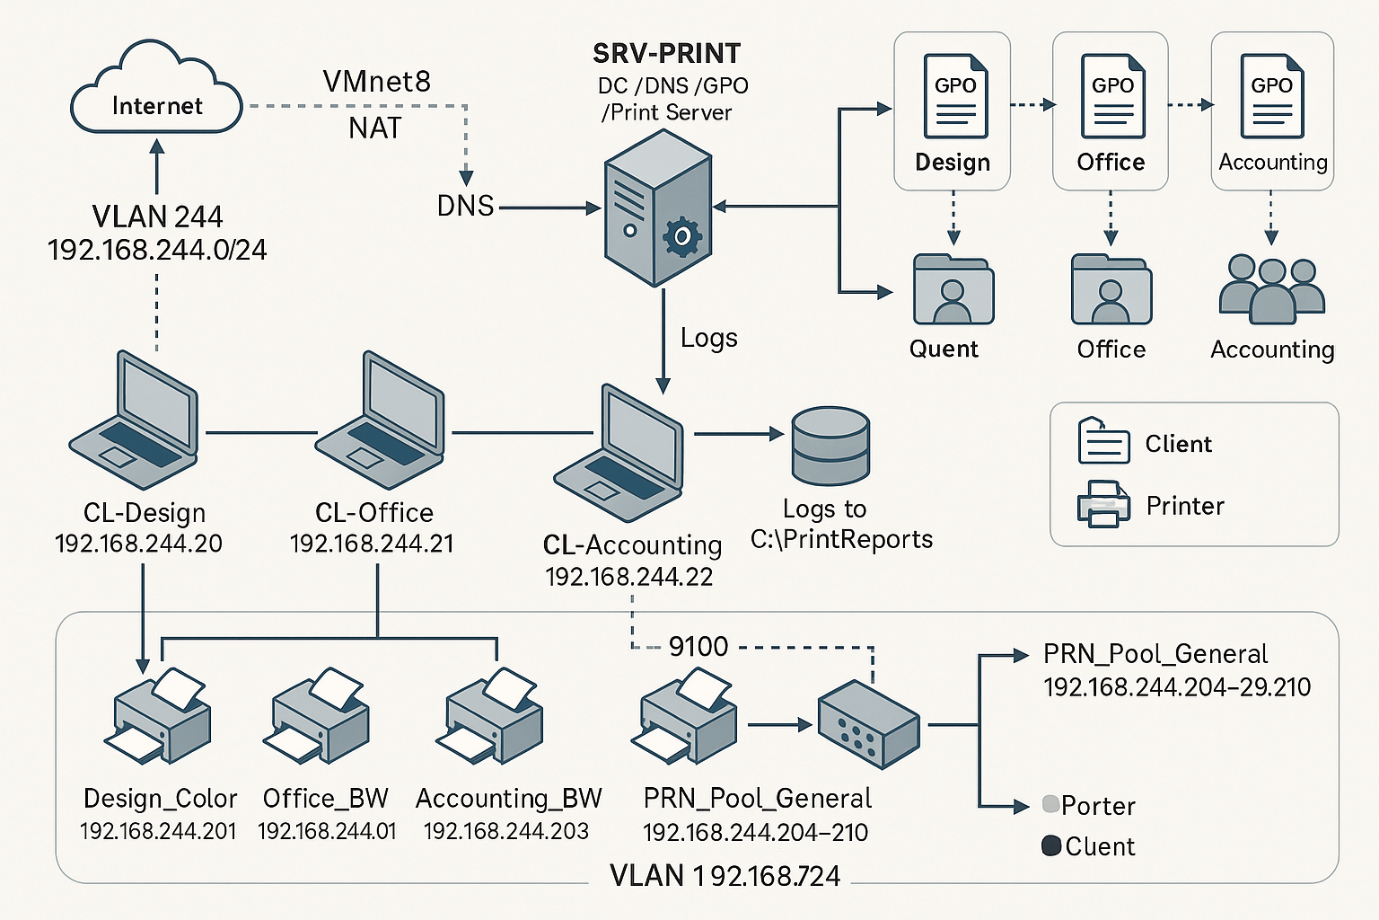
\includegraphics[width=0.92\linewidth]{./media/Sơ đồ cấu trúc hệ thống.png}
    \caption{Sơ đồ cấu trúc tổng thể hệ thống Printer Server}
    \label{fig:system_architecture}
\end{figure}

\subsection{Mô tả thành phần trong kiến trúc}

\begin{itemize}[leftmargin=*,noitemsep,topsep=3pt]
    \item \textbf{1 máy chủ Windows Server 2019 (VMware):}
    \begin{itemize}[noitemsep]
        \item Cài đặt các vai trò: \textbf{Print Server}, \textbf{Active Directory Domain Services}, \textbf{DNS}.
        \item Tham gia domain: \textbf{ABC.local}.
        \item Đóng vai trò máy chủ chính cung cấp dịch vụ in, phân phối máy in và lưu log.
    \end{itemize}

    \item \textbf{3 máy trạm Windows 8.1:}
    \begin{itemize}[noitemsep]
        \item Đại diện cho 3 người dùng thuộc 3 phòng ban: \textit{user\_design}, \textit{user\_office}, \textit{user\_accounting}.
        \item Các máy này nhận máy in tự động thông qua Group Policy.
    \end{itemize}

    \item \textbf{10 máy in vật lý/ảo:}
    \begin{itemize}[noitemsep]
        \item Dải IP sử dụng: \textbf{192.168.244.201 – 192.168.244.210}.
        \item Bao gồm máy in màu, máy in trắng đen và máy in hoá đơn theo nhu cầu từng phòng ban.
    \end{itemize}
\end{itemize}

\begin{table}[htbp]
\centering
\small
\begin{tabular}{|l|p{10.5cm}|}
\hline
\textbf{Thông số} & \textbf{Chi tiết} \\
\hline
Hostname & SRV-PRINT \\
\hline
OS & Windows Server 2019 Datacenter \\
\hline
IP Address & 192.168.244.10/24 \\
\hline
Gateway & 192.168.244.1 \\
\hline
DNS Primary & 192.168.244.10 \\
\hline
DNS Secondary & 8.8.8.8 \\
\hline
Domain & ABC.local \\
\hline
Vai trò & DC + Print Server + DNS + AD DS \\
\hline
Nền tảng & VMware Workstation Pro (Bridged) \\
\hline
\end{tabular}
\caption{Thông số cấu hình Print Server}
\label{tab:print_server_config}
\end{table}

\noindent\textbf{Tóm tắt cấu hình mạng:}
\begin{itemize}[leftmargin=*,noitemsep,topsep=3pt]
    \item \textbf{Server:} Windows Server 2019 (VMware), IP: \textbf{192.168.244.10/24}, Gateway: \textbf{192.168.244.1}.
    \item \textbf{Domain:} \textbf{ABC.local}, tên máy chủ: \textbf{SRV-PRINT}.
    \item \textbf{Client:} Windows 8.1 (đã join domain ABC.local), IP thuộc dải \textbf{192.168.244.x}.
    \item \textbf{Máy in:} các máy in vật lý/ảo sử dụng dải IP \textbf{192.168.244.201–210}.
\end{itemize}

\subsection{Sơ đồ hoạt động hệ thống}
\begin{figure}[htbp]
    \centering
    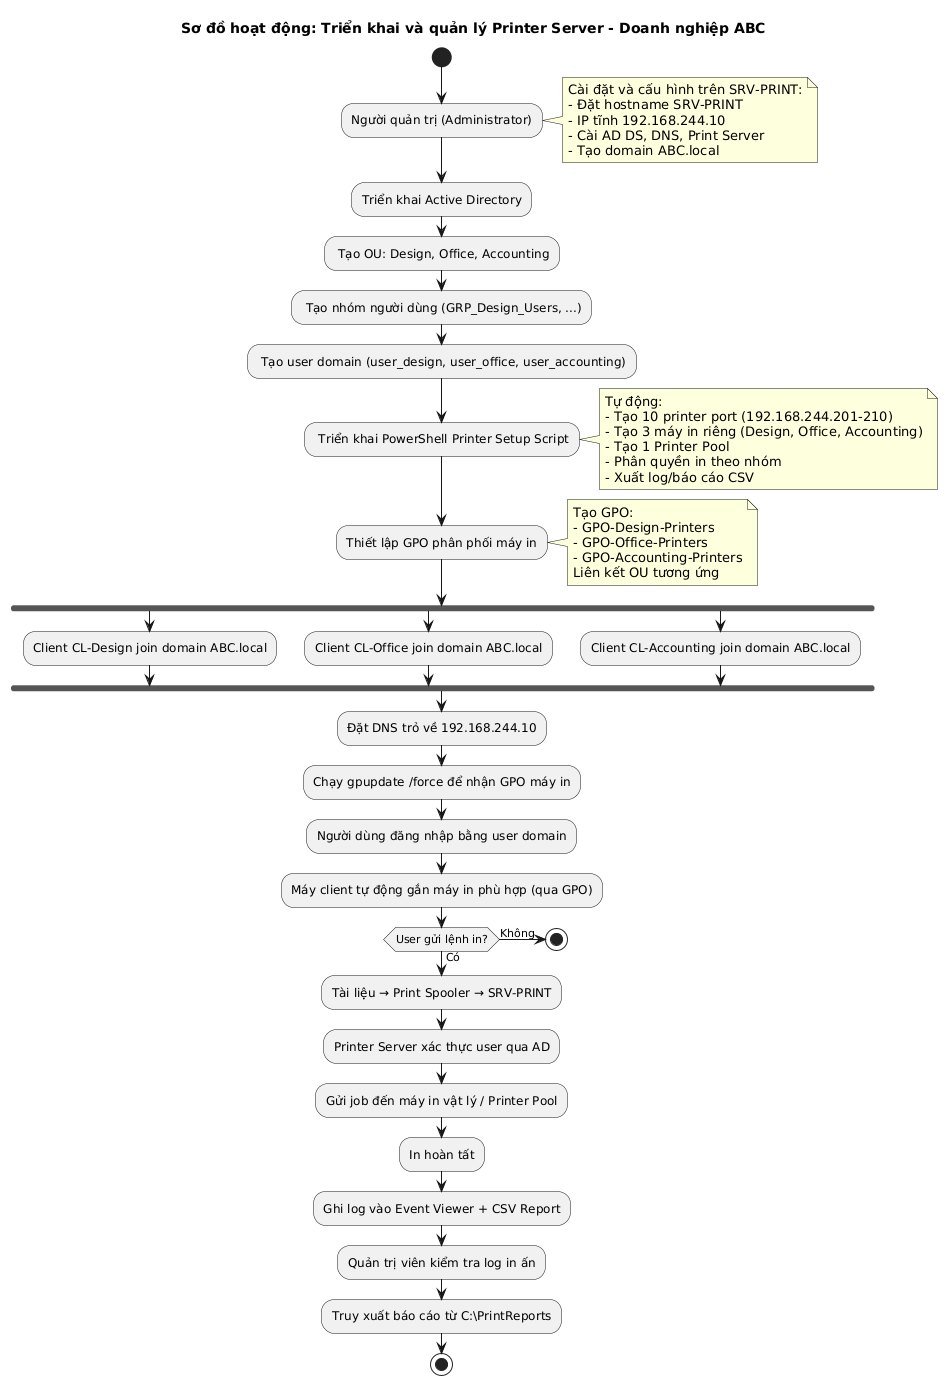
\includegraphics[width=0.88\linewidth]{./media/Sơ đồ hoạt động.png}
    \caption{Sơ đồ hoạt động của hệ thống Printer Server}
    \label{fig:system_flow}
\end{figure}

\section{Cấu trúc Active Directory}
\begin{figure}[htbp]
    \centering
    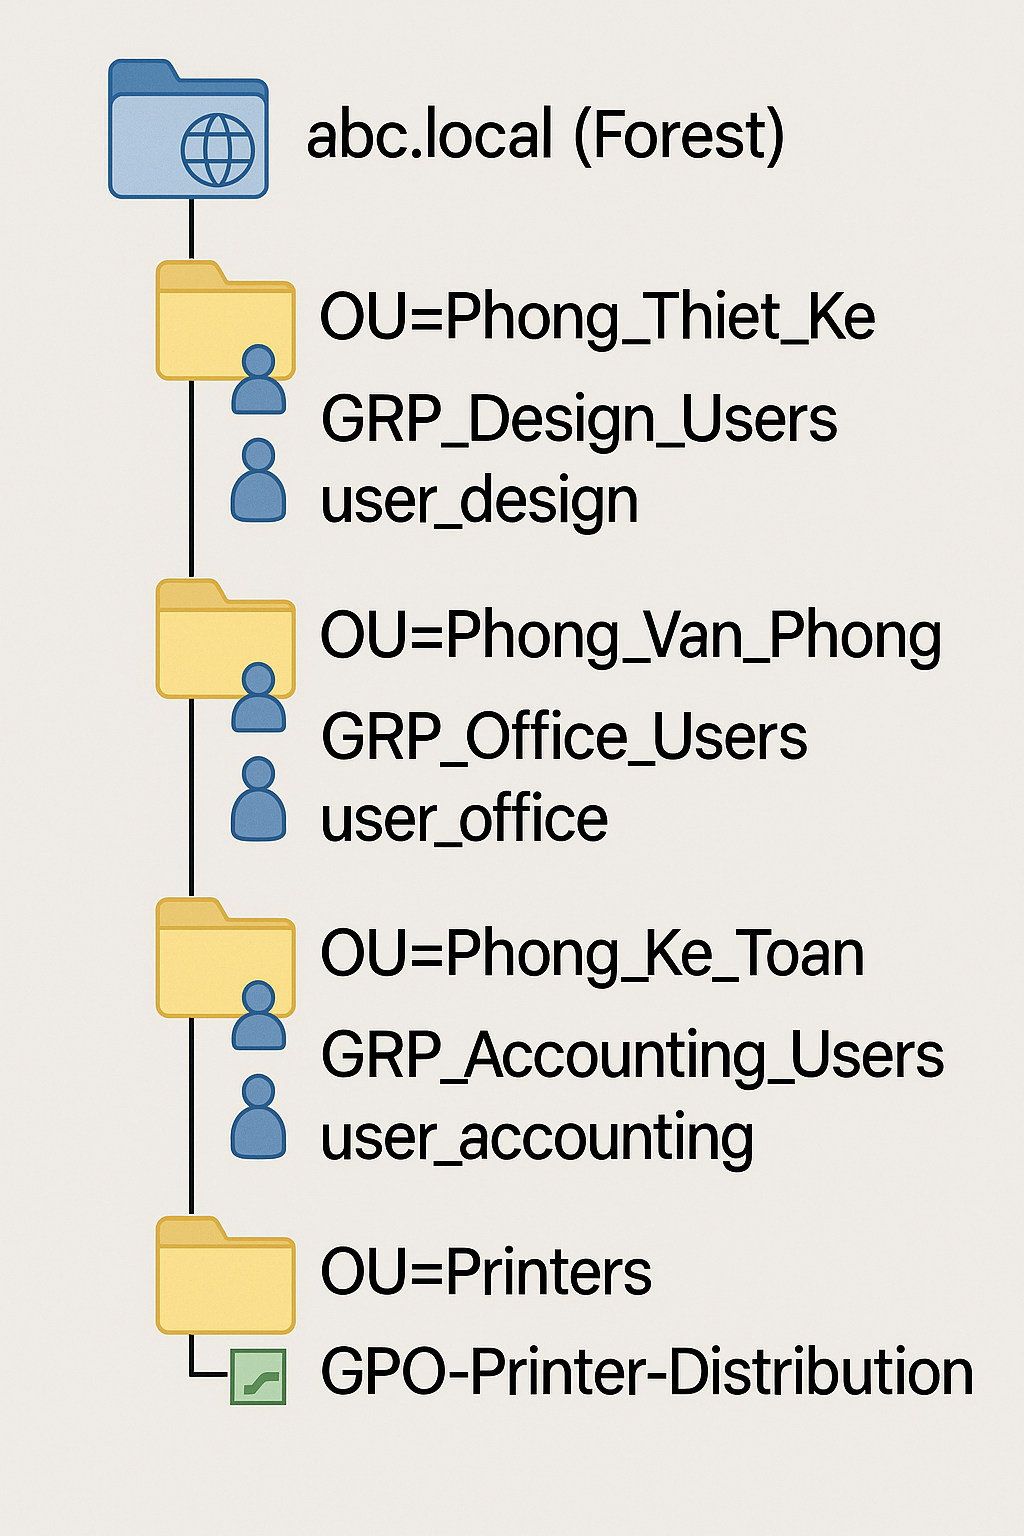
\includegraphics[width=0.72\linewidth]{./media/Cấu trúc Active Directory.png}
    \caption{Cấu trúc Active Directory}
    \label{fig:ad_structure}
\end{figure}

\section{Dải IP và các Port}
\begin{table}[htbp]
\centering
\small
\caption{Phân bổ địa chỉ IP trong mô hình triển khai}
\label{tab:ip-allocation}
\begin{tabular}{|p{2.8cm}|p{2.8cm}|p{3.2cm}|p{4.8cm}|}
\hline
\textbf{Loại thiết bị} & \textbf{Dải IP} & \textbf{Địa chỉ cụ thể} & \textbf{Mục đích sử dụng} \\ \hline
Server & 192.168.244.10/24 & 192.168.244.10 & Máy chủ Print Server (SRV-PRINT) - Windows Server 2019 trên VMware \\ \hline
Gateway & 192.168.244.1 & 192.168.244.1 & Cổng mạng mặc định cho toàn bộ hệ thống \\ \hline
Client computers & 192.168.244.20-99 & 192.168.244.20 \newline 192.168.244.21 \newline 192.168.244.x & Máy trạm Windows 8.1 đã join domain: \newline - user\_design (Phòng Thiết kế) \newline - user\_office (Phòng Văn phòng) \newline - user\_accounting (Phòng Kế toán) \\ \hline
Máy in vật lý/ảo & 192.168.244.201-210 & 192.168.244.201 \newline 192.168.244.202 \newline 192.168.244.203 \newline ... \newline 192.168.244.210 & 10 máy in được phân bổ cho các phòng ban: \newline - Máy in màu cao cấp (Phòng Thiết kế) \newline - Máy in laser trắng đen (Phòng Văn phòng) \newline - Máy in bảo mật (Phòng Kế toán) \newline - Các máy in dự phòng/Printer Pool \\ \hline
\end{tabular}
\end{table}

\subsection*{Thông tin Subnet}
\begin{itemize}[leftmargin=*,noitemsep,topsep=3pt]
    \item \textbf{Subnet Mask:} 255.255.255.0 (/24)
    \item \textbf{Network Address:} 192.168.244.0
    \item \textbf{Broadcast Address:} 192.168.244.255
    \item \textbf{Số IP khả dụng:} 254 địa chỉ (192.168.244.1 - 192.168.244.254)
\end{itemize}

\subsection*{Phân vùng IP đề xuất}
\begin{itemize}[leftmargin=*,noitemsep,topsep=3pt]
    \item \textbf{192.168.244.1-9:} Thiết bị mạng (Gateway, Switch, Router)
    \item \textbf{192.168.244.10-19:} Servers (Domain Controller, Print Server, File Server...)
    \item \textbf{192.168.244.20-199:} Client computers (máy trạm người dùng)
    \item \textbf{192.168.244.200-254:} Thiết bị ngoại vi (Máy in, Scanner, Thiết bị IoT)
\end{itemize}
\vspace{\baselineskip}
\chapter{\textbf{Các bước chuẩn bị}}
\section{Thiết lập Hostname, IP tĩnh trên Server}

\begin{lstlisting}[style=powershell]
# 0.1 Set Hostname = SRV-PRINT
$NewHostname = "SRV-PRINT" 
$CurrentHostname = $env:COMPUTERNAME

if ($CurrentHostname -ne $NewHostname) {
    Write-Host "Changing hostname from $CurrentHostname -> $NewHostname" -ForegroundColor Cyan
    Rename-Computer -NewName $NewHostname -Force
    Write-Host "[OK] Hostname will change after restart" -ForegroundColor Green
} else {
    Write-Host "Hostname is already SRV-PRINT" -ForegroundColor Green
}

# 0.2 Static IP Configuration: 192.168.244.10/24, Gateway: 192.168.244.1
Write-Host "--- Static IP Configuration ---" -ForegroundColor Cyan

$IPAddress = "192.168.244.10" 
$SubnetMask = "255.255.255.0" 
$Gateway = "192.168.244.1" 
$DNS = @("8.8.8.8", "8.8.4.4") # Temporary DNS, DC will be used as DNS later

# Get Ethernet adapter
$NetworkAdapter = Get-NetAdapter | Where-Object {$_.Status -eq "Up"} | Select-Object -First 1

if ($NetworkAdapter) {
    Write-Host "Adapter found: $($NetworkAdapter.Name)" -ForegroundColor Green
    
    # Remove old DHCP configuration
    try {
        Remove-NetIPAddress -InterfaceAlias $NetworkAdapter.Name -Confirm:$false -ErrorAction SilentlyContinue
        Remove-NetRoute -InterfaceAlias $NetworkAdapter.Name -Confirm:$false -ErrorAction SilentlyContinue
    } catch {
        Write-Host " Error removing old configuration: $_" -ForegroundColor Yellow
    }

    # Set Static IP
    try {
        New-NetIPAddress -InterfaceAlias $NetworkAdapter.Name `
            -IPAddress $IPAddress `
            -PrefixLength 24 `
            -DefaultGateway $Gateway `
            -AddressFamily IPv4 `
            -ErrorAction Stop
        Write-Host " IP $IPAddress set successfully" -ForegroundColor Green
    } catch {
        Write-Host " Error setting IP: $_" -ForegroundColor Yellow
    }

    # Set DNS
    try {
        Set-DnsClientServerAddress -InterfaceAlias $NetworkAdapter.Name `
            -ServerAddresses $DNS `
            -ErrorAction Stop
        Write-Host " DNS set successfully" -ForegroundColor Green
    } catch {
        Write-Host " Error setting DNS: $_" -ForegroundColor Yellow
    }

} else {
    Write-Host " Network Adapter not found" -ForegroundColor Red
}

# Verify network configuration
Write-Host "--- Verify Network Configuration ---" -ForegroundColor Cyan
Get-NetIPAddress -AddressFamily IPv4 | Format-Table -AutoSize
Get-DnsClientServerAddress -AddressFamily IPv4 | Format-Table -AutoSize
\end{lstlisting}

\begin{table}[htbp]
\centering
\small
\begin{tabular}{|p{5cm}|p{6cm}|}
\hline
\textbf{Biến} & \textbf{Giá trị} \\
\hline
\texttt{\$IPAddress} & "192.168.244.10" \\
\hline
\texttt{\$SubnetMask} & "255.255.255.0" \\
\hline
\texttt{\$Gateway} & "192.168.244.1" \\
\hline
\texttt{\$DNS1} & "192.168.244.10" \\
\hline
\texttt{\$DNS2} & "8.8.8.8" \\
\hline
\end{tabular}
\caption{Cấu hình IP Static}
\label{tab:ip_static}
\end{table}

\begin{figure}[htbp]
    \centering
    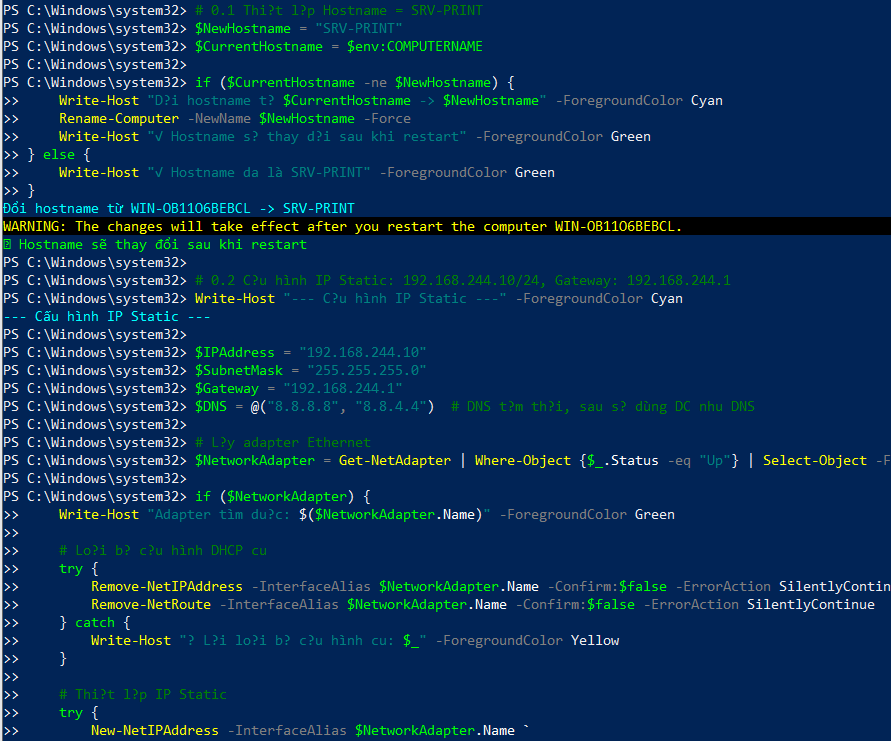
\includegraphics[width=0.78\linewidth]{./media/CẤU HÌNH BAN ĐẦU (HOSTNAME, IP, NETWORK).png}
    \caption{Cấu hình ban đầu}
    \label{fig:initial_config}
\end{figure}

\begin{figure}[htbp]
    \centering
    \begin{minipage}[b]{0.48\textwidth}
        \centering
        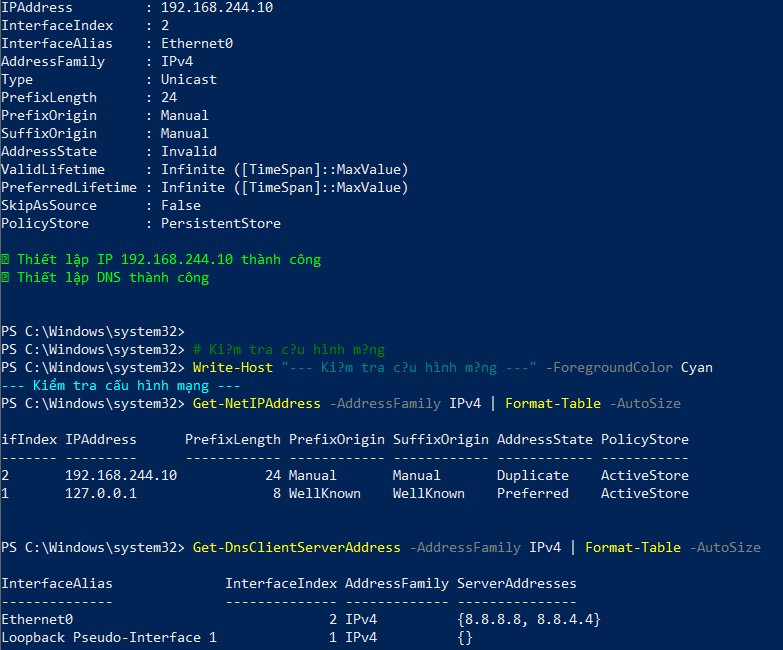
\includegraphics[width=\textwidth]{./media/Thiết lập ip static(1).png}
        \caption{Thiết lập IP static (1)}
        \label{fig:ip_static1}
    \end{minipage}
    \hfill
    \begin{minipage}[b]{0.48\textwidth}
        \centering
        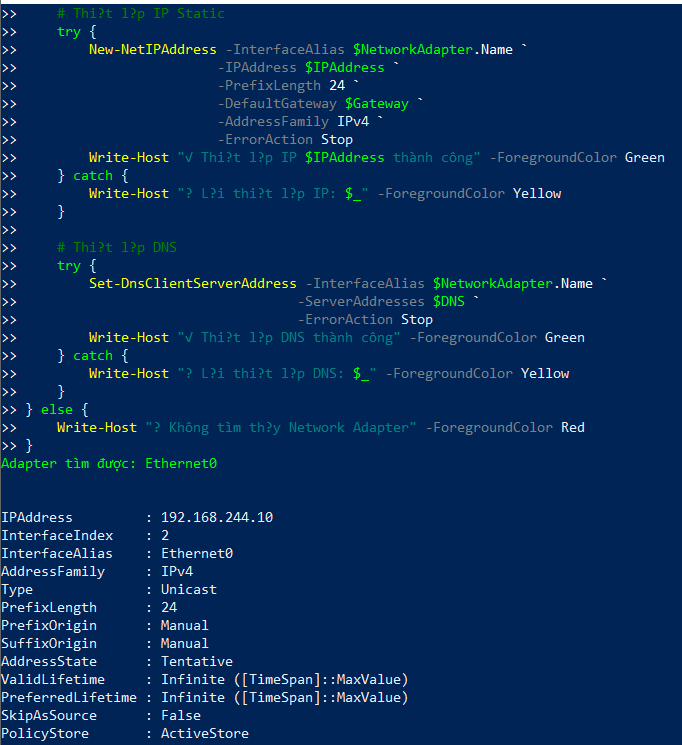
\includegraphics[width=\textwidth]{./media/Thiết lập ip static.png}
        \caption{Thiết lập IP static (2)}
        \label{fig:ip_static2}
    \end{minipage}
\end{figure}

\section{Cài đặt Server, AD, DS, DNS}
\subsection{Cấu hình ban đầu trên Server (Windows Server 2019)}

\begin{lstlisting}[style=powershell]
# 1.1 Install Print and Document Services Role
Write-Host "=== STEP 1: Install Print Server Role ===" -ForegroundColor Cyan
Install-WindowsFeature -Name Print-Server -IncludeManagementTools -Restart:$false
Write-Host "[OK] Print Server installed" -ForegroundColor Green

# 1.2 Check Print Server status
Get-WindowsFeature -Name Print-Server | Select-Object Name, Installed

# 1.3 Start Print Spooler service
Write-Host "=== STEP 2: Start Print Spooler service ===" -ForegroundColor Cyan
Start-Service -Name Spooler
Set-Service -Name Spooler -StartupType Automatic
Get-Service -Name Spooler
\end{lstlisting}

\begin{figure}[htbp]
    \centering
    \begin{minipage}[b]{0.48\textwidth}
        \centering
        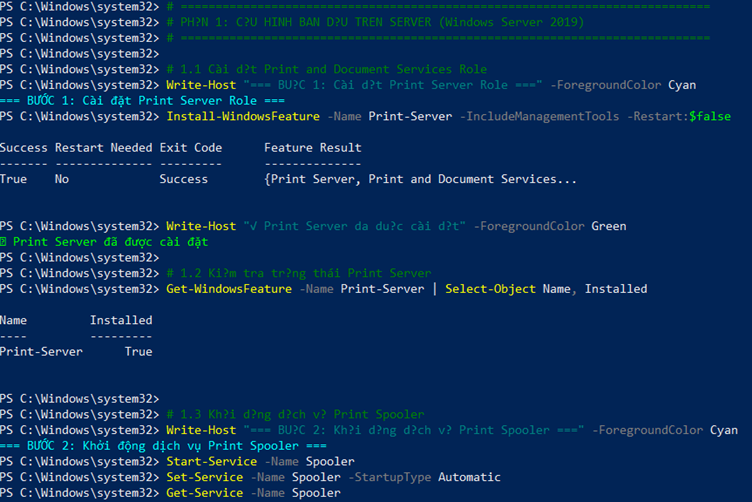
\includegraphics[width=\textwidth]{./media/CH Ban Đầu.png}
        \caption{Cấu hình ban đầu (1)}
        \label{fig:config_initial1}
    \end{minipage}
    \hfill
    \begin{minipage}[b]{0.48\textwidth}
        \centering
        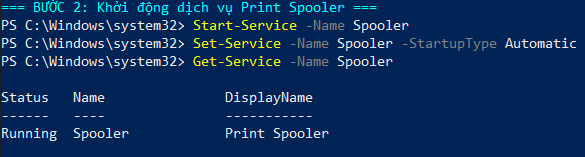
\includegraphics[width=\textwidth]{./media/Cấu hình winserv2019(1).png}
        \caption{Cấu hình ban đầu (2)}
        \label{fig:config_initial2}
    \end{minipage}
\end{figure}

\subsection{Cài đặt Active Directory Domain Controller}

\begin{lstlisting}[style=powershell]
# 1.1 Install AD DS Role
try {
    Install-WindowsFeature -Name AD-Domain-Services -IncludeManagementTools -Restart:$false -ErrorAction Stop
    Write-Host "[OK] AD Domain Services installed" -ForegroundColor Green
} catch {
    Write-Host "[!] AD DS installed or error: $_" -ForegroundColor Yellow
}

# 1.2 Install DNS Server (required for DC)
try {
    Install-WindowsFeature -Name DNS -IncludeManagementTools -Restart:$false -ErrorAction Stop
    Write-Host "[OK] DNS Server installed" -ForegroundColor Green
} catch {
    Write-Host "[!] DNS Server installed or error: $_" -ForegroundColor Yellow
}

# 1.3 Create Forest and Domain: ABC.local
Write-Host "--- Create Domain ABC.local ---" -ForegroundColor Cyan
$DomainName = "ABC.local" 
$SafeModePW = ConvertTo-SecureString -AsPlainText "Manh31102005" -Force

try {
    Install-ADDSForest -DomainName $DomainName `
    -SafeModeAdministratorPassword $SafeModePW `
    -InstallDNS `
    -NoRebootOnCompletion:$false `
    -Force `
    -WarningAction SilentlyContinue `
    -ErrorAction Stop
    
    Write-Host "[OK] Domain $DomainName created successfully" -ForegroundColor Green
    Write-Host "[OK] Server will automatically restart to complete setup" -ForegroundColor Green
    Start-Sleep -Seconds 5
}
catch {
    Write-Host "[!] Error creating Domain: $_" -ForegroundColor Yellow
}
\end{lstlisting}

\begin{figure}[htbp]
    \centering
    \begin{minipage}[b]{0.48\textwidth}
        \centering
        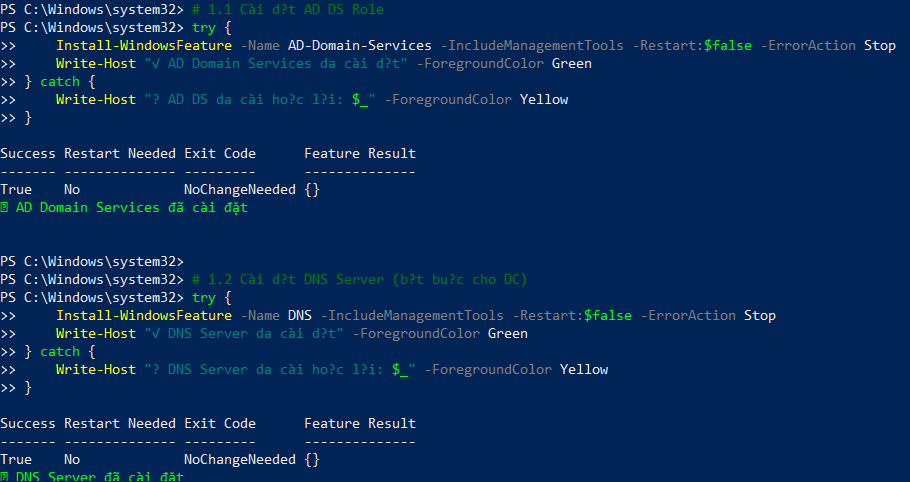
\includegraphics[width=\textwidth]{./media/Cài đặt AD DS role.png}
        \caption{Cài đặt AD DS role (1)}
        \label{fig:adds_install1}
    \end{minipage}
    \hfill
    \begin{minipage}[b]{0.48\textwidth}
        \centering
        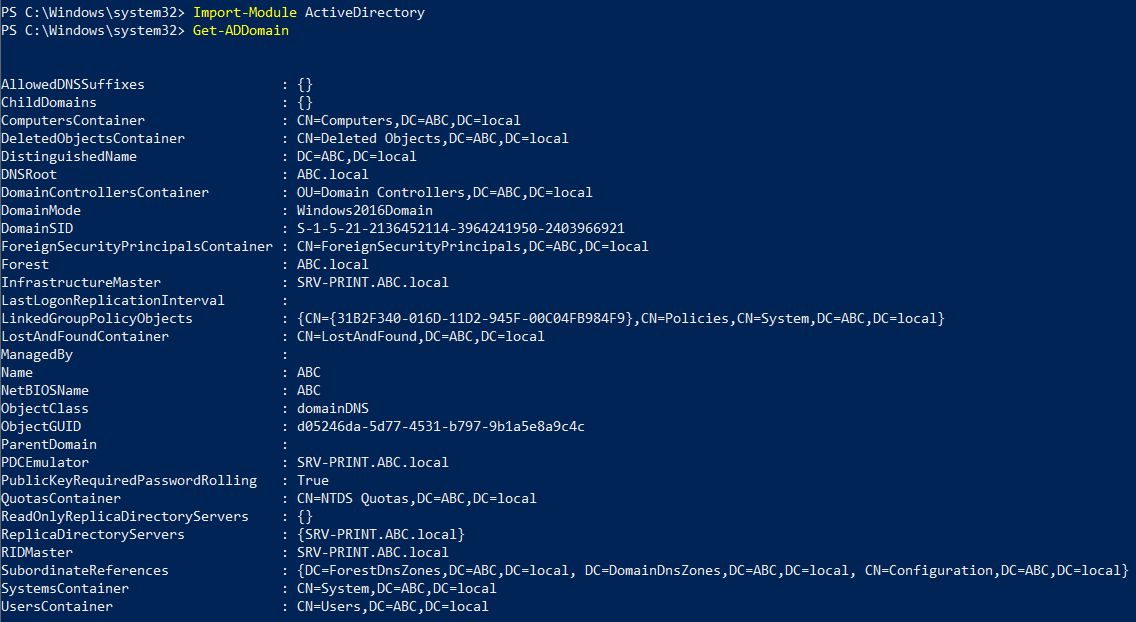
\includegraphics[width=\textwidth]{./media/Cài đặt AD DS role(1).png}
        \caption{Cài đặt AD DS role (2)}
        \label{fig:adds_install2}
    \end{minipage}
\end{figure}

\section{Tạo cấu trúc nhóm Active Directory}

\textbf{Tạo nhóm AD cho từng phòng ban}

\begin{itemize}[leftmargin=*,noitemsep,topsep=3pt]
    \item \textbf{Cài RSAT-AD-PowerShell (module ActiveDirectory)}
\end{itemize}

\begin{lstlisting}[style=powershell]
Install-WindowsFeature AD-Domain-Services, RSAT-AD-PowerShell -IncludeManagementTools
\end{lstlisting}

\begin{figure}[htbp]
    \centering
    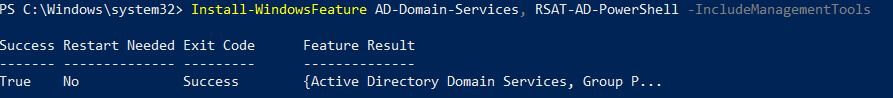
\includegraphics[width=0.72\linewidth]{./media/Cài RSAT-AD-PowerShell (module ActiveDirectory).png}
    \caption{Cài RSAT-AD-PowerShell}
    \label{fig:rsat_install}
\end{figure}

\begin{itemize}[leftmargin=*,noitemsep,topsep=3pt]
    \item \textbf{Tạo Nhóm AD cho từng phòng ban}
\end{itemize}

\begin{lstlisting}[style=powershell]
$DomainDN = "DC=ABC,DC=local" 
$OUPath = "OU=PrinterGroups,OU=PrinterManagement,$DomainDN" 
$UserOUPath = "OU=Users,OU=PrinterManagement,$DomainDN" 

Write-Host "--- Create Test Users ---" -ForegroundColor Cyan

$Password = ConvertTo-SecureString -AsPlainText "Manh31102005" -Force

$Users = @(
    @{
        UserName="user_design"
        GivenName="User"
        Surname="Design"
        GroupName="GRP_Design"
        Description="Design Department User"
    }, 
    @{
        UserName="user_office"
        GivenName="User"
        Surname="Office"
        GroupName="GRP_Office"
        Description="Office Department User"
    }, 
    @{
        UserName="user_accounting"
        GivenName="User"
        Surname="Accounting"
        GroupName="GRP_Accounting"
        Description="Accounting Department User"
    }
)

foreach ($user in $Users) {
    try {
        New-ADUser -SamAccountName $user.UserName `
            -UserPrincipalName "$($user.UserName)@ABC.local" `
            -GivenName $user.GivenName `
            -Surname $user.Surname `
            -Name "$($user.GivenName) $($user.Surname)" `
            -DisplayName "$($user.GivenName) $($user.Surname)" `
            -Description $user.Description `
            -AccountPassword $Password `
            -Enabled $true `
            -PasswordNeverExpires $true `
            -Path $UserOUPath `
            -ErrorAction Stop
            
        Write-Host "[OK] User '$($user.UserName)' created successfully" -ForegroundColor Green

        # Add user to corresponding group
        Add-ADGroupMember -Identity $user.GroupName -Members $user.UserName -ErrorAction Stop
        
        Write-Host " [OK] Added '$($user.UserName)' to group '$($user.GroupName)'" -ForegroundColor Green

    } catch {
        Write-Host "[!] Error with user '$($user.UserName)': $_" -ForegroundColor Yellow
    }
}
\end{lstlisting}

\begin{figure}[htbp]
    \centering
    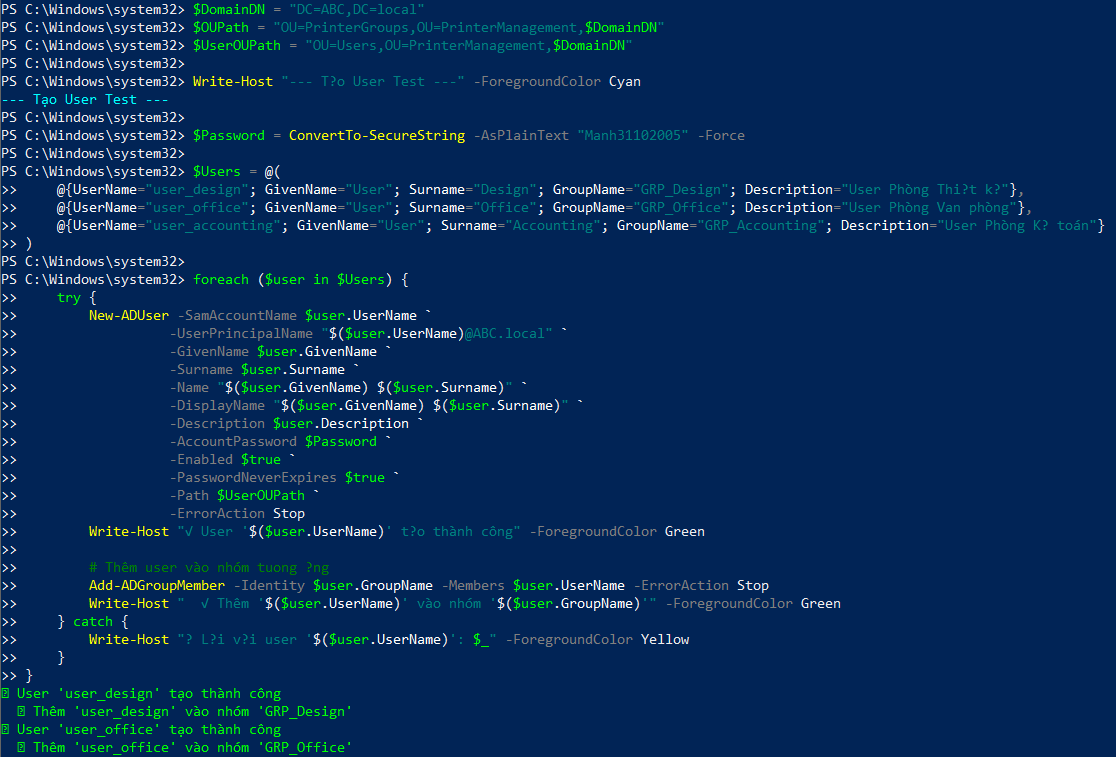
\includegraphics[width=0.78\textwidth]{./media/Tạo Nhóm AD cho từng phòng ban.png}
    \caption{Tạo Nhóm AD cho từng phòng ban}
    \label{fig:ad_groups}
\end{figure}

\chapter{\textbf{Tạo nhóm và người dùng}}
\section{Tạo nhóm theo từng phòng ban}

\begin{lstlisting}[style=powershell]
$DomainDN = "DC=ABC,DC=local"
$OUPath = "OU=PrinterGroups,OU=PrinterManagement,$DomainDN"
$UserOUPath = "OU=Users,OU=PrinterManagement,$DomainDN"

Write-Host "--- Tao User Test ---" -ForegroundColor Cyan

$Password = ConvertTo-SecureString -AsPlainText "Manh31102005" -Force

$Users = @(
    @{UserName="user_design"; GivenName="User"; Surname="Design"; GroupName="GRP_Design"; Description="User Phong Thiet ke"},
    @{UserName="user_office"; GivenName="User"; Surname="Office"; GroupName="GRP_Office"; Description="User Phong Van phong"},
    @{UserName="user_accounting"; GivenName="User"; Surname="Accounting"; GroupName="GRP_Accounting"; Description="User Phong Ke toan"}
)
\end{lstlisting}

\section{Tạo User tương ứng}

\begin{lstlisting}[style=powershell]
foreach ($user in $Users) {
    try {
        New-ADUser -SamAccountName $user.UserName `
                  -UserPrincipalName "$($user.UserName)@ABC.local" `
                  -GivenName $user.GivenName `
                  -Surname $user.Surname `
                  -Name "$($user.GivenName) $($user.Surname)" `
                  -DisplayName "$($user.GivenName) $($user.Surname)" `
                  -Description $user.Description `
                  -AccountPassword $Password `
                  -Enabled $true `
                  -PasswordNeverExpires $true `
                  -Path $UserOUPath `
                  -ErrorAction Stop
        Write-Host "[OK] User '$($user.UserName)' tao thanh cong" -ForegroundColor Green
        
        # Them user vao nhom tuong ung
        Add-ADGroupMember -Identity $user.GroupName -Members $user.UserName -ErrorAction Stop
        Write-Host " [OK] Them '$($user.UserName)' vao nhom '$($user.GroupName)'" -ForegroundColor Green
    } catch {
        Write-Host "[!] Loi voi user '$($user.UserName)': $_" -ForegroundColor Yellow
    }
}
\end{lstlisting}

\begin{figure}[htbp]
    \centering
    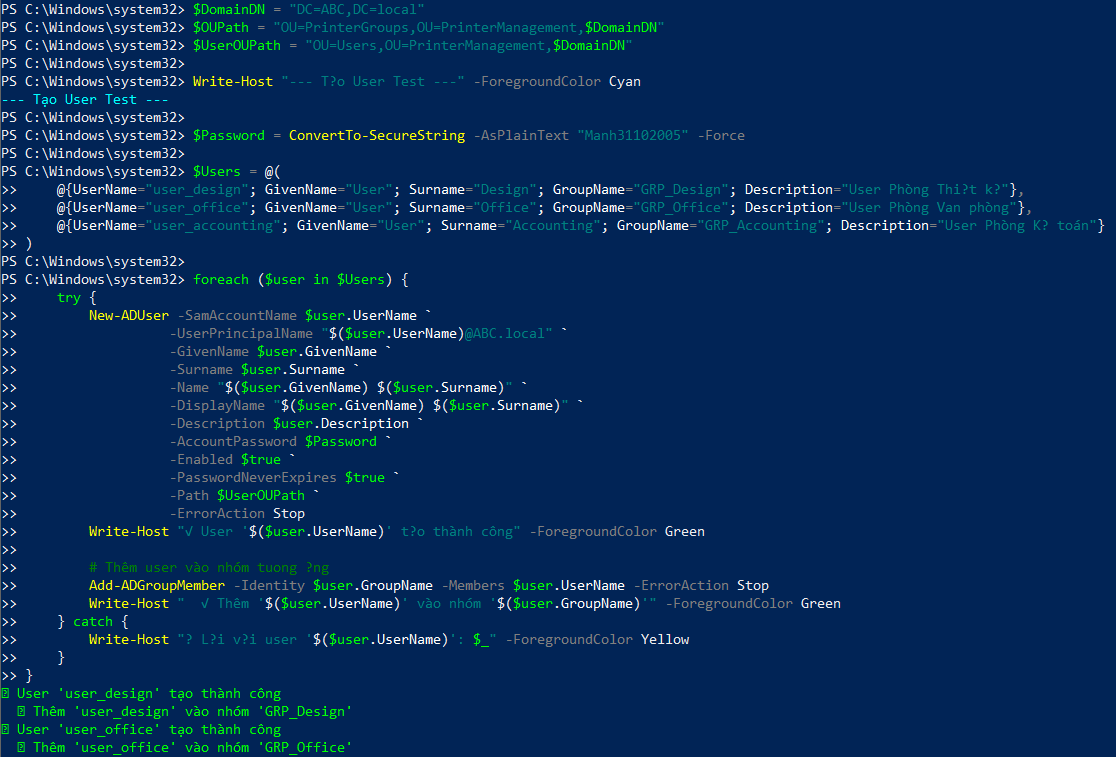
\includegraphics[width=0.78\textwidth]{./media/Tạo Nhóm AD cho từng phòng ban.png}
    \caption{Tạo Nhóm AD và thêm các User vào từng phòng ban}
    \label{fig:users_groups}
\end{figure}
\vspace{\baselineskip}

\chapter{\textbf{Triển khai Port và Driver}}
\section{Tạo TCP/IP port cho máy in}

\begin{lstlisting}[style=powershell]
Write-Host "=== Create TCP/IP Printer Ports ===" -ForegroundColor Cyan

$PrinterIPRange = 201..210

foreach ($i in $PrinterIPRange) {
    $IP = "192.168.244.$i" 
    $PortName = "IP_192.168.244.$i"
    
    try {
        Add-PrinterPort -Name $PortName `
            -PrinterHostAddress $IP `
            -ErrorAction Stop
            
        Write-Host "[OK] Printer port '$PortName' ($IP) created successfully" -ForegroundColor Green
    } catch {
        if ($_ -like "*already exists*") {
            Write-Host "[!] Port '$PortName' already exists" -ForegroundColor Yellow
        } else {
            Write-Host "[!] Error with port '$PortName': $_" -ForegroundColor Yellow
        }
    }
}

# Check port list
Write-Host "`n=== Printer Port List ===" -ForegroundColor Cyan

Get-PrinterPort | Where-Object {$_.Name -like "IP_192.168.244.*"} | Select-Object Name, PrinterHostAddress | Format-Table -AutoSize
\end{lstlisting}

\begin{figure}[htbp]
    \centering
    \begin{minipage}[b]{0.48\textwidth}
        \centering
        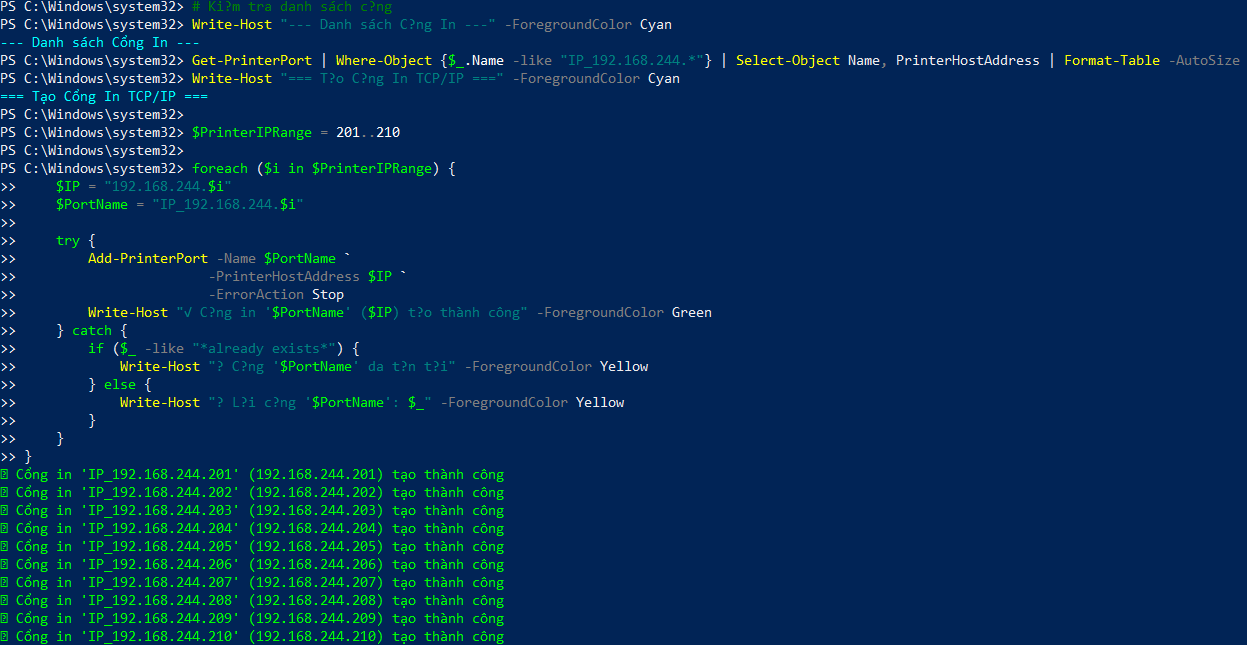
\includegraphics[width=\textwidth]{./media/TẠO CÁC CỔNG IN (PORTS).png}
        \caption{Tạo các cổng Port để in (1)}
        \label{fig:ports1}
    \end{minipage}
    \hfill
    \begin{minipage}[b]{0.48\textwidth}
        \centering
        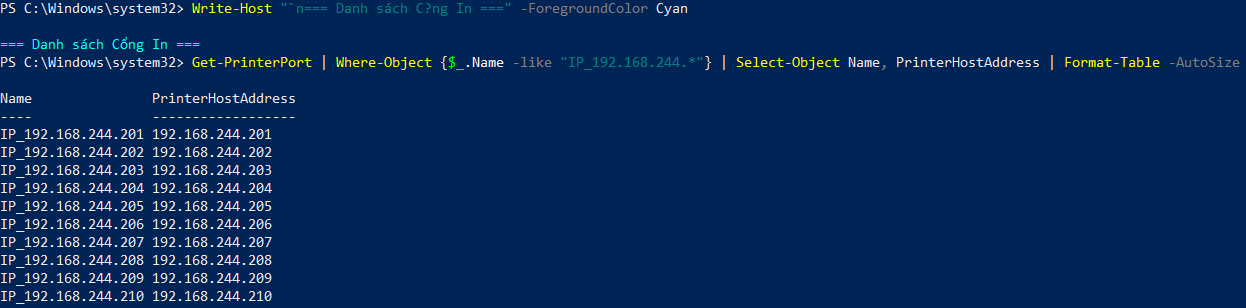
\includegraphics[width=\textwidth]{./media/TẠO CÁC CỔNG IN (PORTS)(1).png}
        \caption{Tạo các cổng Port để in (2)}
        \label{fig:ports2}
    \end{minipage}
\end{figure}

\section{Kiểm tra và cài driver}
\subsection{Cài đặt HP Universal Print Driver PCL6 64-bit}

\noindent\textbf{Lý do chọn HP Universal Print Driver PCL6 64-bit:}

\begin{itemize}[leftmargin=*,noitemsep,topsep=3pt]
    \item \textbf{Phù hợp môi trường doanh nghiệp:} Driver Universal của HP (PCL6) hỗ trợ nhiều model máy in HP khác nhau, giúp triển khai máy in cho nhiều phòng ban mà không cần cài từng loại driver riêng biệt.
    \item \textbf{Tương thích với nhiều thiết bị:} HP UPD được thiết kế để hoạt động ổn định với phần lớn các máy in HP, phù hợp với lab kiểu doanh nghiệp có nhiều máy in.
    \item \textbf{Hỗ trợ chuẩn in phổ biến:} PCL6 là ngôn ngữ in tiêu chuẩn, giúp chia sẻ tài nguyên và tạo pool máy in ảo dễ dàng.
    \item \textbf{Dễ dàng triển khai tự động hóa:} Driver universal đơn giản hóa cấu hình, phân phối qua PowerShell, Group Policy (GPO).
    \item \textbf{Tăng tính thực tế:} Dùng driver universal cho nhiều phòng ban, phân quyền, chia pool, theo dõi log phù hợp với vận hành doanh nghiệp thực tế.
    \item \textbf{Tiết kiệm thời gian:} Không lo lỗi tương thích khi cập nhật driver hoặc di chuyển máy in.
\end{itemize}

\begin{lstlisting}[style=powershell]
$driverPath = "C:\PrinterDrivers\HP-PCL6"
\end{lstlisting}

\noindent\textbf{Tìm file .INF chính:}

\begin{lstlisting}[style=powershell]
Write-Host "`n[STEP 1] Finding main .INF file..." -ForegroundColor Yellow

$allInfFiles = Get-ChildItem -Path $driverPath -Filter "*.inf" -Recurse

Write-Host "All .INF files:" -ForegroundColor Cyan
$infList = @()

for ($i = 0; $i -lt $allInfFiles.Count; $i++) {
    $inf = $allInfFiles[$i]
    $size = $inf.Length / 1KB
    
    Write-Host " [$i] $($inf.Name) ($([Math]::Round($size, 2)) KB) - Path: $($inf.Directory.Name)" -ForegroundColor Gray
    $infList += $inf
}

$rootInfs = Get-ChildItem -Path $driverPath -MaxDepth 1 -Filter "*.inf" -ErrorAction SilentlyContinue

if ($rootInfs) {
    Write-Host "`n[OK] Found .INF file in root folder:" -ForegroundColor Green
    foreach ($inf in $rootInfs) {
        Write-Host " > $($inf.Name)" -ForegroundColor Green
    }
    $mainInf = $rootInfs[0]
} else {
    Write-Host "`n[INFO] .INF file is in a subdirectory, selecting the largest file..." -ForegroundColor Yellow
    
    $mainInf = $allInfFiles | Sort-Object Length -Descending | Select-Object -First 1
    Write-Host " > $($mainInf.Name)" -ForegroundColor Cyan
}

Write-Host "`n[OK] Main .INF file used: $($mainInf.FullName)" -ForegroundColor Green
\end{lstlisting}

\begin{figure}[htbp]
    \centering
    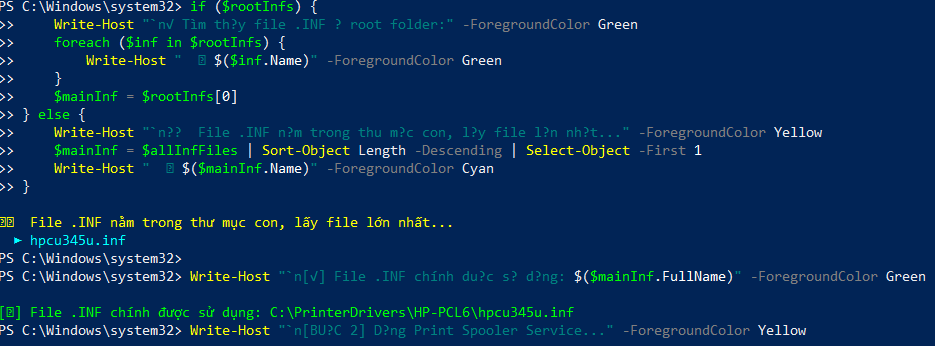
\includegraphics[width=0.78\textwidth]{./media/Tìm file .INF chính.png}
    \caption{Tìm file .INF chính}
    \label{fig:inf_file}
\end{figure}

\noindent\textbf{Dừng Print Spool:}

\begin{lstlisting}[style=powershell]
Write-Host "`n[STEP 2] Stop Print Spooler Service..." -ForegroundColor Yellow

$spooler = Get-Service -Name "Spooler"

if ($spooler.Status -eq "Running") {
    Write-Host "[STOP] Stopping Spooler..." -ForegroundColor Yellow
    Stop-Service -Name "Spooler" -Force
    Start-Sleep -Seconds 3
    Write-Host "[OK] Spooler stopped" -ForegroundColor Green
}
\end{lstlisting}

\begin{figure}[htbp]
    \centering
    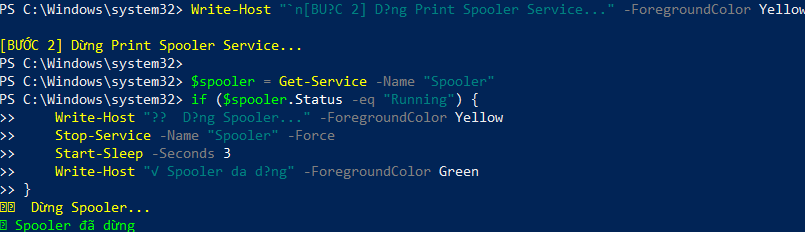
\includegraphics[width=0.78\textwidth]{./media/Dừng Print Spool.png}
    \caption{Dừng Print Spool}
    \label{fig:stop_spool}
\end{figure}

\noindent\textbf{Cài Driver bằng PNPUTIL:}

\begin{lstlisting}[style=powershell]
Write-Host "`n[STEP 3] Installing driver using pnputil..." -ForegroundColor Yellow
Write-Host " > INF File: $($mainInf.Name)" -ForegroundColor Cyan
Write-Host " > Path: $($mainInf.FullName)" -ForegroundColor Cyan
 
# Install driver from main .INF file
Write-Host "`n [*] Installing driver..." -ForegroundColor Cyan

$installOutput = & pnputil.exe -i -a "$($mainInf.FullName)" 2>&1
 
Write-Host "`n [Output from pnputil]:" -ForegroundColor Gray
$installOutput | ForEach-Object { Write-Host "    $($_.ToString())" -ForegroundColor Gray }
 
Write-Host "`n[OK] Installation command executed" -ForegroundColor Green
\end{lstlisting}

\begin{figure}[htbp]
    \centering
    \begin{minipage}[b]{0.48\textwidth}
        \centering
        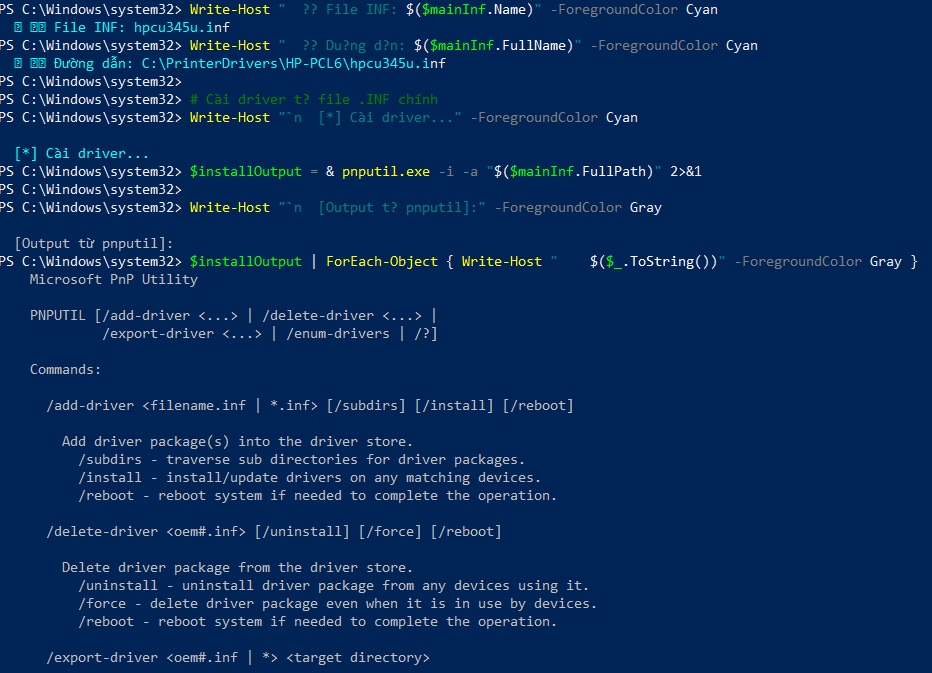
\includegraphics[width=\textwidth]{./media/Cài Driver bằng PNPUTIL.png}
        \caption{Cài Driver bằng PNPUTIL (1)}
        \label{fig:pnputil1}
    \end{minipage}
    \hfill
    \begin{minipage}[b]{0.48\textwidth}
        \centering
        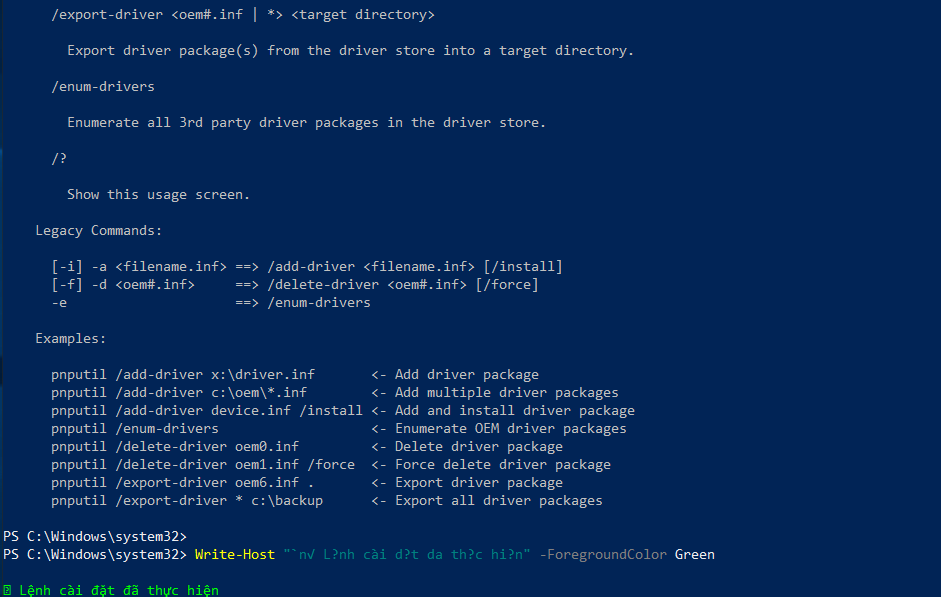
\includegraphics[width=\textwidth]{./media/Cài Driver bằng PNPUTIL(1).png}
        \caption{Cài Driver bằng PNPUTIL (2)}
        \label{fig:pnputil2}
    \end{minipage}
\end{figure}

\noindent\textbf{Khởi động lại Print Spool:}

\begin{lstlisting}[style=powershell]
Write-Host "`n[STEP 4] Restart Print Spooler..." -ForegroundColor Yellow

Start-Service -Name "Spooler"
Start-Sleep -Seconds 5

$spoolerStatus = (Get-Service -Name "Spooler").Status
Write-Host "[OK] Spooler Status: $spoolerStatus" -ForegroundColor Green
\end{lstlisting}

\begin{figure}[htbp]
    \centering
    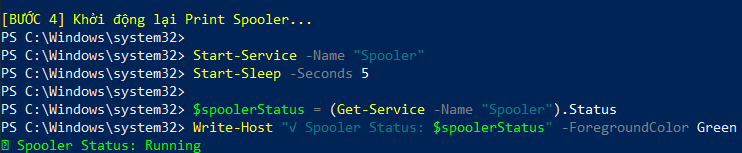
\includegraphics[width=0.78\textwidth]{./media/Khởi động lại Print Spool.png}
    \caption{Khởi động lại Print Spool}
    \label{fig:restart_spool}
\end{figure}

\noindent\textbf{Kiểm tra driver đã được cài đặt:}

\begin{lstlisting}[style=powershell]
Write-Host "`n[STEP 5] Checking installed drivers..." -ForegroundColor Yellow
 
$drivers = Get-PrinterDriver
 
if ($drivers.Count -eq 0) {
    Write-Host "[!] No drivers found!" -ForegroundColor Red
} else {
    Write-Host "`n=== PRINTER DRIVER LIST ===" -ForegroundColor Green
    
    $drivers | Select-Object @{Name="No.";Expression={$drivers.IndexOf($_)+1}}, Name, Version, PrinterEnvironment | Format-Table -AutoSize
 
    # Find HP driver
    $hpDriver = $drivers | Where-Object {$_.Name -like "*HP*" -or $_.Name -like "*Universal*" -or $_.Name -like "*PCL*"}
    
    if ($hpDriver) {
        Write-Host "`n[OK] HP DRIVER FOUND" -ForegroundColor Green
        Write-Host " Driver Name: $($hpDriver.Name)" -ForegroundColor Green
        Write-Host " Version: $($hpDriver.Version)" -ForegroundColor Green
        Write-Host " Environment: $($hpDriver.PrinterEnvironment)" -ForegroundColor Green
    } else {
        Write-Host "`n[!] HP driver not found, but other drivers exist:" -ForegroundColor Yellow
        $drivers | Select-Object Name | Format-Table -AutoSize
    }
}
\end{lstlisting}

\begin{figure}[htbp]
    \centering
    \begin{minipage}[b]{0.48\textwidth}
        \centering
        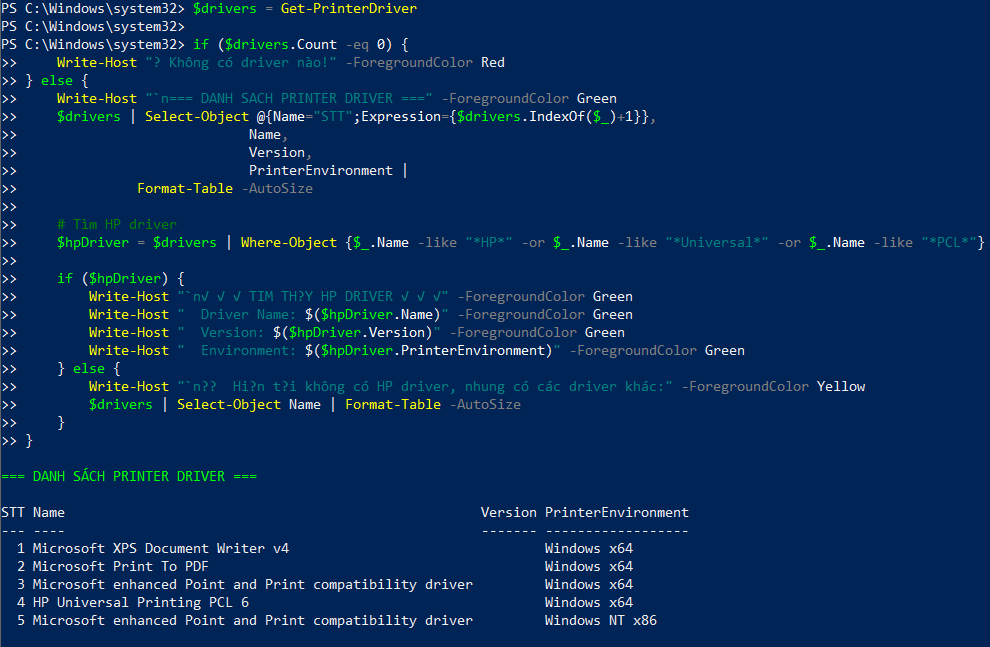
\includegraphics[width=\textwidth]{./media/Kiểm tra driver đã được cài đặt.png}
        \caption{Kiểm tra driver (1)}
        \label{fig:check_driver1}
    \end{minipage}
    \hfill
    \begin{minipage}[b]{0.48\textwidth}
        \centering
        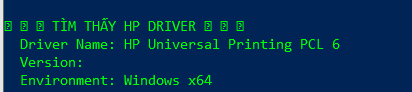
\includegraphics[width=\textwidth]{./media/Kiểm tra driver đã được cài đặt(1).png}
        \caption{Kiểm tra driver (2)}
        \label{fig:check_driver2}
    \end{minipage}
\end{figure}
\vspace{\baselineskip}

\chapter{\textbf{Tạo máy in theo từng phòng ban}}
\section{Add Printer tương ứng cho từng phòng ban}

\begin{lstlisting}[style=powershell]
Write-Host "`n=== BUOC 7: Tao May In Chia Se ===" -ForegroundColor Cyan

# Kiem tra driver co san
$AvailableDriver = Get-PrinterDriver -Name $DriverName -ErrorAction SilentlyContinue

if (-not $AvailableDriver) {
    Write-Host "[!] Driver '$DriverName' khong tim thay" -ForegroundColor Yellow
    $DriverName = "Generic / Text Only"
    Write-Host "Su dung driver thay the: $DriverName" -ForegroundColor Cyan
}

# Tao 10 may in don le
Write-Host "`n--- Tao 10 May In ---" -ForegroundColor Cyan

$PrinterInfo = @(
    @{Name="PRN_Design_01"; Description="May in Mau - Phong Thiet ke 1"; IP="192.168.244.201"; Department="Design"; Location="Tang 3, Phong Thiet ke"},
    @{Name="PRN_Design_02"; Description="May in Mau - Phong Thiet ke 2"; IP="192.168.244.202"; Department="Design"; Location="Tang 3, Phong Thiet ke"},
    @{Name="PRN_Office_01"; Description="May in B/W - Van phong 1"; IP="192.168.244.203"; Department="Office"; Location="Tang 2, Phong Van phong"},
    @{Name="PRN_Office_02"; Description="May in B/W - Van phong 2"; IP="192.168.244.204"; Department="Office"; Location="Tang 2, Phong Van phong"},
    @{Name="PRN_Office_03"; Description="May in B/W - Van phong 3"; IP="192.168.244.205"; Department="Office"; Location="Tang 2, Phong Van phong"},
    @{Name="PRN_Accounting_01"; Description="May in Hoa don - Ke toan 1"; IP="192.168.244.206"; Department="Accounting"; Location="Tang 1, Phong Ke toan"},
    @{Name="PRN_Accounting_02"; Description="May in Hoa don - Ke toan 2"; IP="192.168.244.207"; Department="Accounting"; Location="Tang 1, Phong Ke toan"},
    @{Name="PRN_Reserve_01"; Description="May in Du phong 1"; IP="192.168.244.208"; Department="Reserve"; Location="Tang 1, Phong May"},
    @{Name="PRN_Reserve_02"; Description="May in Du phong 2"; IP="192.168.244.209"; Department="Reserve"; Location="Tang 1, Phong May"},
    @{Name="PRN_Test_01"; Description="May in Test"; IP="192.168.244.210"; Department="Test"; Location="Tang 1, IT"}
)

foreach ($printer in $PrinterInfo) {
    $PortName = "IP_$($printer.IP)"
    
    try {
        Add-Printer -Name $printer.Name `
                   -DriverName $DriverName `
                   -PortName $PortName `
                   -ErrorAction Stop
        
        # Chia se may in
        Set-Printer -Name $printer.Name -Shared $true -ErrorAction SilentlyContinue
        
        Write-Host "[OK] May in '$($printer.Name)' tao thanh cong" -ForegroundColor Green
    } catch {
        Write-Host "[!] May in '$($printer.Name)' loi: $_" -ForegroundColor Yellow
    }
}

# Kiem tra danh sach may in
Write-Host "`n--- Danh sach May In Chia Se ---" -ForegroundColor Cyan
Get-Printer | Select-Object Name, Description, Location, Shared | Format-Table -AutoSize
\end{lstlisting}

\begin{figure}[htbp]
    \centering
    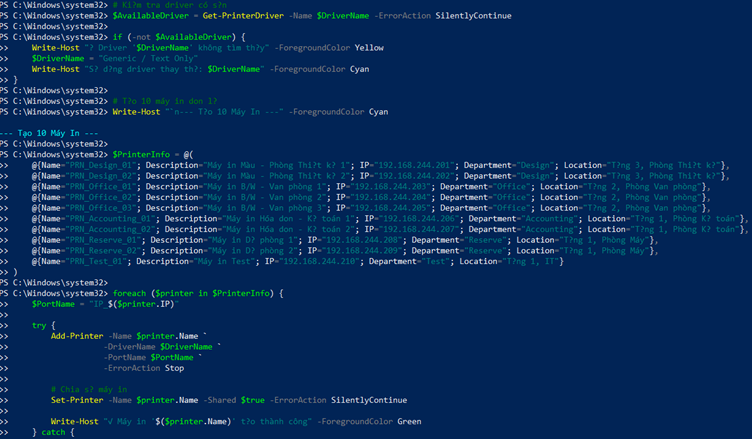
\includegraphics[width=0.78\textwidth]{./media/DS may in.png}
    \caption{Kiểm tra danh sách máy in đã tạo}
    \label{fig:printer_list}
\end{figure}

\section{Tạo Printer Pool khi cần}

\begin{lstlisting}[style=powershell]
$DriverName = "HP Universal Printing PCL 6"
$PoolName = "PRN_Pool_Office"
$PoolPrinterList = @("PRN_Office_01", "PRN_Office_02", "PRN_Office_03")
 
# Get ports from printers in the pool list
$PoolPorts = @()
foreach ($prn in $PoolPrinterList) {
    $Port = (Get-Printer -Name $prn -ErrorAction SilentlyContinue).PortName
    if ($Port) {
        $PoolPorts += $Port
    }
}
 
Write-Host "Found $($PoolPorts.Count) ports for the pool" -ForegroundColor Cyan
 
if ($PoolPorts.Count -ge 2) {
    try {
        # Create Printer Pool (Basic creation with first port)
        Add-Printer -Name $PoolName `
                   -DriverName $DriverName `
                   -PortName $PoolPorts[0] `
                   -ErrorAction Stop
        
        # Share the printer
        Set-Printer -Name $PoolName -Shared $true
        
        # OPTIONAL: Uncomment the line below to actually enable Pooling across all found ports
        # Set-Printer -Name $PoolName -PortName ($PoolPorts -join ",")

        Write-Host "[OK] Pool '$PoolName' created successfully" -ForegroundColor Green
        Write-Host " Ports in pool:" -ForegroundColor Cyan
        foreach ($port in $PoolPorts) {
            Write-Host "    - $port" -ForegroundColor Cyan
        }
    } catch {
        Write-Host "[!] Error creating Pool: $_" -ForegroundColor Yellow
    }
} else {
    Write-Host "[!] Not enough printers for the pool" -ForegroundColor Yellow
}
 
# Check
Get-Printer -Name $PoolName -ErrorAction SilentlyContinue | Format-Table
\end{lstlisting}

\begin{figure}[htbp]
    \centering
    \begin{minipage}[b]{0.48\textwidth}
        \centering
        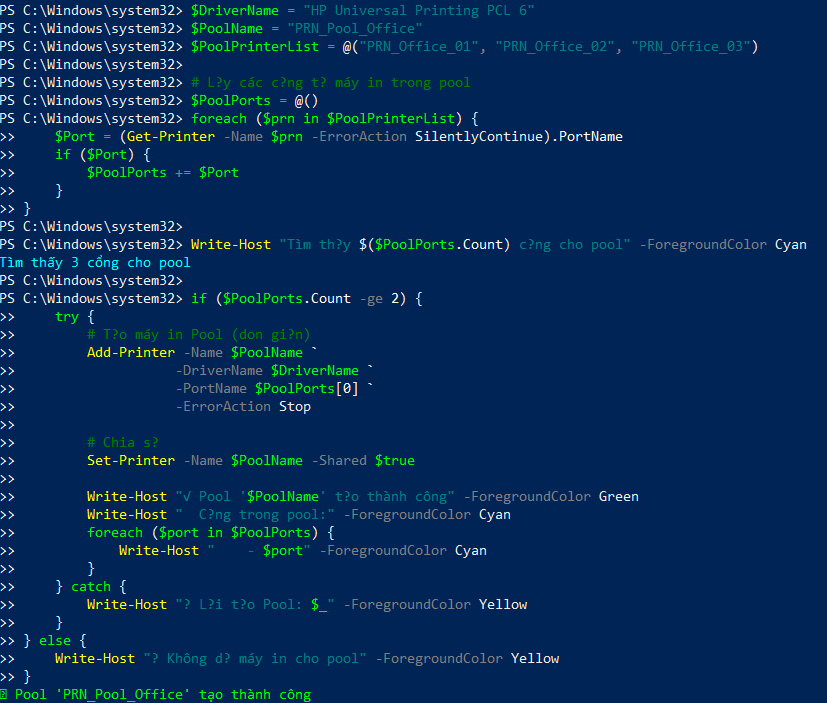
\includegraphics[width=\textwidth]{./media/TẠO PRINTER POOL CHO PHÒNG VĂN PHÒNG.png}
        \caption{Tạo Printer Pool (1)}
        \label{fig:pool1}
    \end{minipage}
    \hfill
    \begin{minipage}[b]{0.48\textwidth}
        \centering
        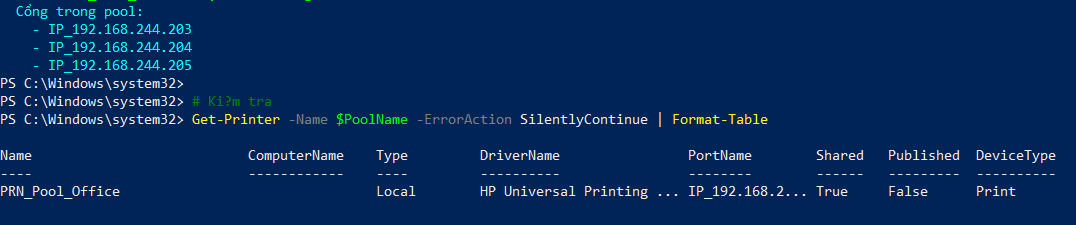
\includegraphics[width=\textwidth]{./media/TẠO PRINTER POOL CHO PHÒNG VĂN PHÒNG(1).png}
        \caption{Tạo Printer Pool (2)}
        \label{fig:pool2}
    \end{minipage}
\end{figure} 
\chapter{\textbf{Phân quyền và kiểm soát truy cập}}
\section{Phân quyền cho máy in bằng ICACLS}
\begin{lstlisting}[style=powershell]
$Domain = "ABC"
 
# Configure printer permissions
$PermissionConfig = @(
    @{Name="PRN_Design_01"; Group="GRP_Design"},
    @{Name="PRN_Design_02"; Group="GRP_Design"},
    @{Name="PRN_Office_01"; Group="GRP_Office"},
    @{Name="PRN_Office_02"; Group="GRP_Office"},
    @{Name="PRN_Office_03"; Group="GRP_Office"},
    @{Name="PRN_Accounting_01"; Group="GRP_Accounting"},
    @{Name="PRN_Accounting_02"; Group="GRP_Accounting"}
)
 
foreach ($printer in $PermissionConfig) {
    Write-Host "Configuring: $($printer.Name)" -ForegroundColor Cyan
    
    # Grant permissions using icacls
    & icacls "\\.\pipe\$($printer.Name)" /inheritance:r `
        /grant:f "${Domain}\$($printer.Group):(OI)(CI)(F)" `
        /grant:f "SYSTEM:(OI)(CI)(F)" `
        /grant:f "Administrators:(OI)(CI)(F)" 2>$null
        
    Write-Host "  [OK] Done" -ForegroundColor Green
}
 
# Configure Pool permissions
Write-Host "Configuring: PRN_Pool_Office" -ForegroundColor Cyan
 
& icacls "\\.\pipe\PRN_Pool_Office" /inheritance:r `
    /grant:f "${Domain}\GRP_Design:(OI)(CI)(F)" `
    /grant:f "${Domain}\GRP_Office:(OI)(CI)(F)" `
    /grant:f "${Domain}\GRP_Accounting:(OI)(CI)(F)" `
    /grant:f "SYSTEM:(OI)(CI)(F)" `
    /grant:f "Administrators:(OI)(CI)(F)" 2>$null
    
Write-Host "  [OK] Done" -ForegroundColor Green
\end{lstlisting}

\begin{figure}[htbp]
    \centering
    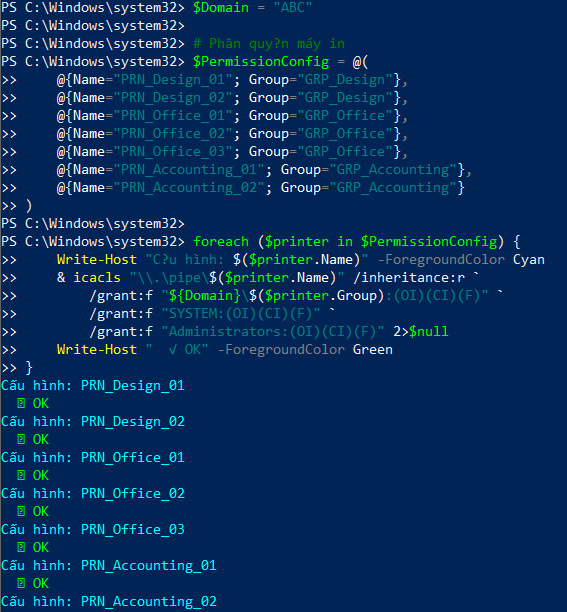
\includegraphics[width=0.75\textwidth]{./media/PHÂN QUYỀN CHO MÁY IN.png}
    \vspace{-0.3cm}
    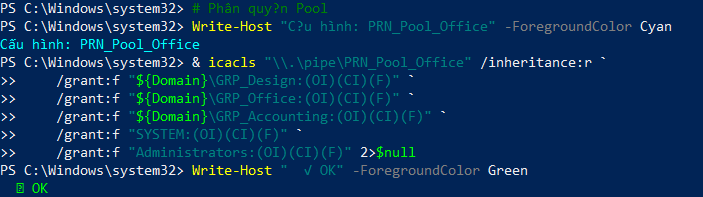
\includegraphics[width=0.75\textwidth]{./media/PHÂN QUYỀN CHO MÁY IN(1).png}
    \caption{Phân quyền cho máy in}
    \label{fig:mirrored_vd_19}
\end{figure}

\noindent\textbf{Giải thích tham số:}
\begin{itemize}[topsep=2pt,itemsep=1pt,parsep=0pt]
    \item (OI): Object Inherit – quyền áp dụng cho đối tượng con khi có.
    \item (CI): Container Inherit – quyền áp dụng cho container con.
    \item (F): Full control – toàn quyền sử dụng.
\end{itemize}

\noindent\textit{Các nhóm user AD (Active Directory):}
\begin{itemize}[topsep=2pt,itemsep=1pt,parsep=0pt]
    \item \textit{GRP\_Design\_Users: Chỉ được dùng máy in của phòng thiết kế và máy in pool.}
    \item \textit{GRP\_Office\_Users: Chỉ được dùng máy in của phòng văn phòng và máy in pool.}
    \item \textit{GRP\_Accounting\_Users: Chỉ được dùng máy in của phòng kế toán và máy in pool.}
\end{itemize}

\begin{table}[htbp]
    \centering
    \caption{Phân quyền máy in theo nhóm}
    \label{tab:printer_permissions}
    \begin{tabular}{|l|l|p{4.5cm}|}
        \hline
        \textbf{Tên máy in} & \textbf{Nhóm được cấp quyền} & \textbf{Mô tả quyền} \\ \hline
        PRN\_Design\_Color\_01 & GRP\_Design\_Users & Toàn quyền phòng thiết kế \\ \hline
        PRN\_Office\_BW\_01 & GRP\_Office\_Users & Toàn quyền phòng văn phòng \\ \hline
        PRN\_Accounting\_BW\_01 & GRP\_Accounting\_Users & Toàn quyền phòng kế toán \\ \hline
        PRN\_Pool\_General & Cả 3 nhóm phòng ban & Dùng chung, chia tải \\ \hline
    \end{tabular}
\end{table}

\section{Thiết lập độ ưu tiên cho các máy in (Priority)}
\begin{lstlisting}[style=powershell]
$PriorityConfig = @(
    @{Printer="PRN_Design_01"; Priority=50},
    @{Printer="PRN_Design_02"; Priority=50},
    @{Printer="PRN_Office_01"; Priority=25},
    @{Printer="PRN_Office_02"; Priority=25},
    @{Printer="PRN_Office_03"; Priority=25},
    @{Printer="PRN_Pool_Office"; Priority=30},
    @{Printer="PRN_Accounting_01"; Priority=75},
    @{Printer="PRN_Accounting_02"; Priority=75}
)

foreach ($config in $PriorityConfig) {
    try {
        Set-Printer -Name $config.Printer -Priority $config.Priority -ErrorAction Stop
        Write-Host "[OK] $($config.Printer) - Priority: $($config.Priority)" -ForegroundColor Green
    } catch {
        Write-Host "[!] Error setting priority $($config.Printer): $_" -ForegroundColor Yellow
    }
}

# Check priority
Write-Host "`n--- Priority List ---" -ForegroundColor Cyan
Get-Printer | Where-Object {$_.Name -like "PRN_*"} | Select-Object Name, Priority | Format-Table
\end{lstlisting}

\begin{figure}[htbp]
    \centering
    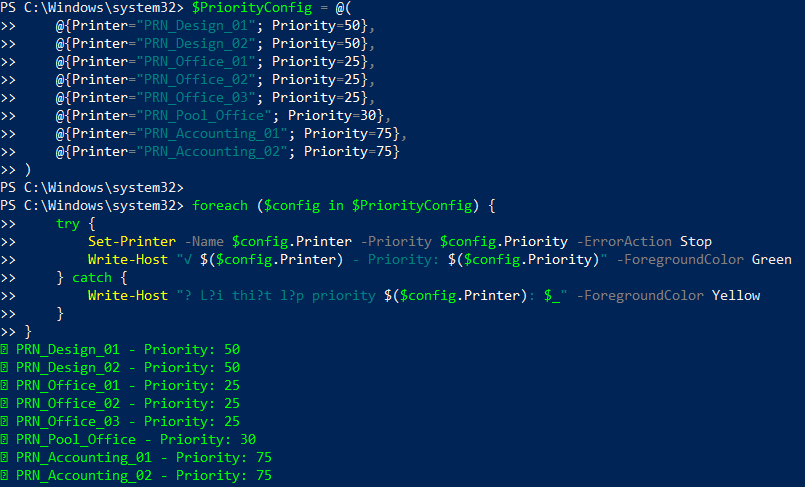
\includegraphics[width=0.7\textwidth]{./media/THIẾT LẬP ĐỘ ƯU TIÊN CHO MÁY IN.png}
    \vspace{-0.3cm}
    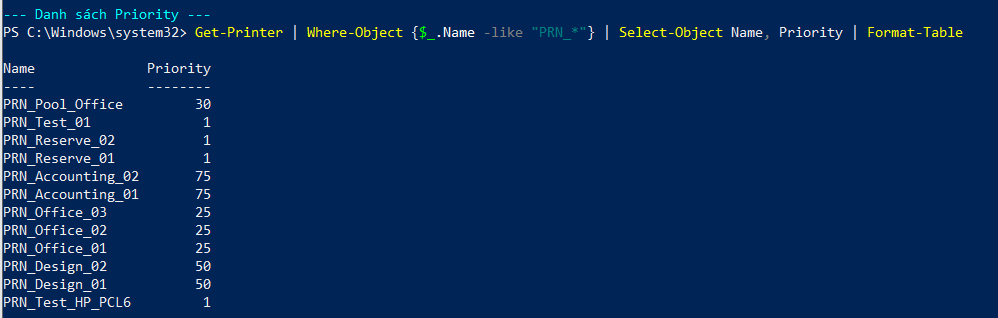
\includegraphics[width=0.7\textwidth]{./media/THIẾT LẬP ĐỘ ƯU TIÊN CHO MÁY IN(1).png}
    \caption{Thiết lập độ ưu tiên cho các máy in}

    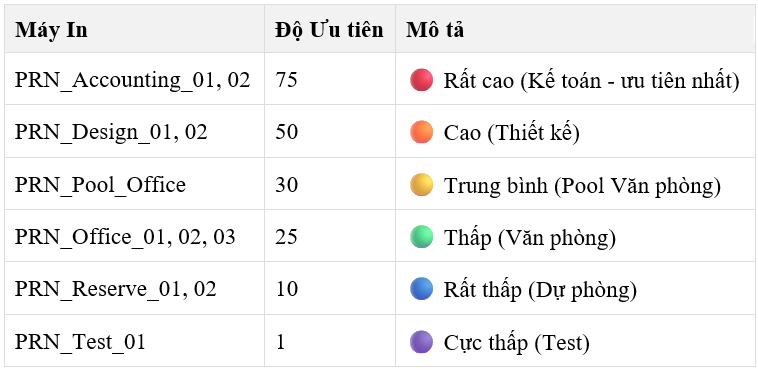
\includegraphics[width=0.85\textwidth]{./media/DUT.png}
    \caption{Độ ưu tiên của các máy in}
    \label{fig:mirrored_vd_16}
\end{figure}
\vspace{\baselineskip}


\chapter{\textbf{Phân phối máy in qua Group Policy}}
\section{Tạo Logon Script}
\begin{lstlisting}[style=powershell]
# Client Printer Deployment Script
$ClientDeployScript = @'
# Script runs on Client Windows 8.1 (Logon Script)
# Purpose: Automatically connect printers based on user AD group
 
Write-Host "=== Deploying Printers for User ===" -ForegroundColor Cyan
 
# Get current user information
$CurrentUser = [System.Security.Principal.WindowsIdentity]::GetCurrent().Name
Write-Host "Current User: $CurrentUser" -ForegroundColor Green
 
# Get user AD groups
$UserGroups = @()
try {
    $SamAccount = $CurrentUser.Split("\")[-1]
    $ADUser = Get-ADUser -Identity $SamAccount -Properties MemberOf -ErrorAction Stop
    $UserGroups = $ADUser.MemberOf | ForEach-Object {
        (Get-ADGroup -Identity $_ -ErrorAction SilentlyContinue).Name
    }
    Write-Host "User Groups: $($UserGroups -join ', ')" -ForegroundColor Green
} catch {
    Write-Host "Warning: Could not retrieve AD groups: $_" -ForegroundColor Yellow
}
 
# Define printers by group
$PrinterMapping = @{
    "GRP_Design" = @("\\SRV-PRINT\PRN_Design_01", "\\SRV-PRINT\PRN_Design_02");
    "GRP_Office" = @("\\SRV-PRINT\PRN_Office_01", "\\SRV-PRINT\PRN_Office_02", "\\SRV-PRINT\PRN_Office_03", "\\SRV-PRINT\PRN_Pool_Office");
    "GRP_Accounting" = @("\\SRV-PRINT\PRN_Accounting_01", "\\SRV-PRINT\PRN_Accounting_02")
}
 
# Connect printers matching user group
$ConnectedPrinters = @()
foreach ($group in $UserGroups) {
    if ($PrinterMapping.ContainsKey($group)) {
        Write-Host "Processing group: $group" -ForegroundColor Cyan
        foreach ($printer in $PrinterMapping[$group]) {
            try {
                Add-Printer -ConnectionName $printer -ErrorAction Stop
                $ConnectedPrinters += $printer
                Write-Host "[OK] Connected printer: $printer" -ForegroundColor Green
            } catch {
                Write-Host "[!] Failed to connect $printer : $_" -ForegroundColor Yellow
            }
        }
    }
}
 
# Display list of connected printers
Write-Host "`n=== Available Printers ===" -ForegroundColor Cyan
Get-Printer | Where-Object {$_.Type -eq "Connection"} | Select-Object Name, ComputerName | Format-Table -AutoSize
 
Write-Host "[OK] Printer deployment completed for $CurrentUser" -ForegroundColor Green
'@
 
# Save client script
$ScriptPath = "C:\PrinterScripts"
if (-not (Test-Path $ScriptPath)) {
    New-Item -ItemType Directory -Path $ScriptPath -Force | Out-Null
    Write-Host "[OK] Created folder $ScriptPath" -ForegroundColor Green
}
 
$ClientScriptFile = "$ScriptPath\Deploy-Printers-Client.ps1"
$ClientDeployScript | Out-File -FilePath $ClientScriptFile -Encoding UTF8 -Force
Write-Host "[OK] Client script saved at: $ClientScriptFile" -ForegroundColor Green
 
# Share script folder for client download
Write-Host "`n--- Share Script Folder ---" -ForegroundColor Cyan
 
$ShareName = "PrinterScripts"
try {
    New-SmbShare -Name $ShareName -Path $ScriptPath -FullAccess "Authenticated Users" -ErrorAction Stop
    Write-Host "[OK] Folder $ShareName shared successfully" -ForegroundColor Green
} catch {
    Write-Host "[!] Folder $ShareName already shared or error: $_" -ForegroundColor Yellow
}
\end{lstlisting}

\begin{figure}[htbp]
    \centering
    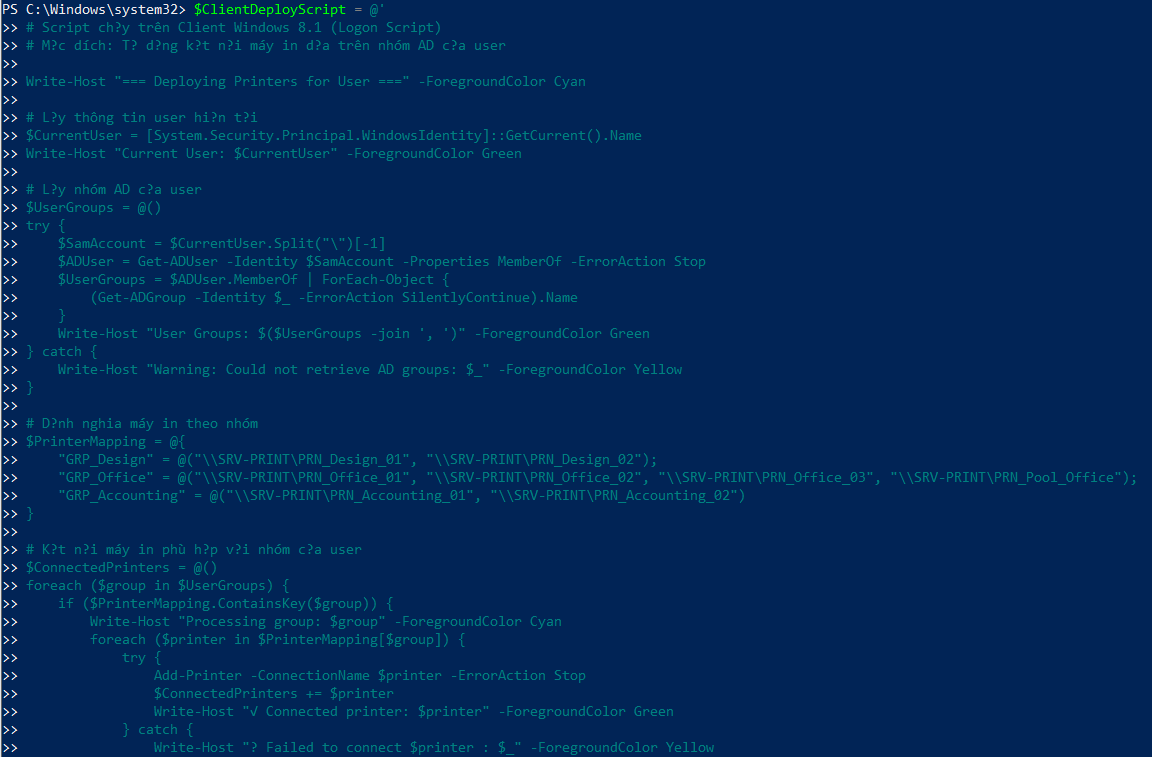
\includegraphics[width=0.7\textwidth]{./media/TẠO SCRIPT PHÂN PHỐI MÁY IN ĐẾN CLIENT.png}
    \vspace{-0.25cm}
    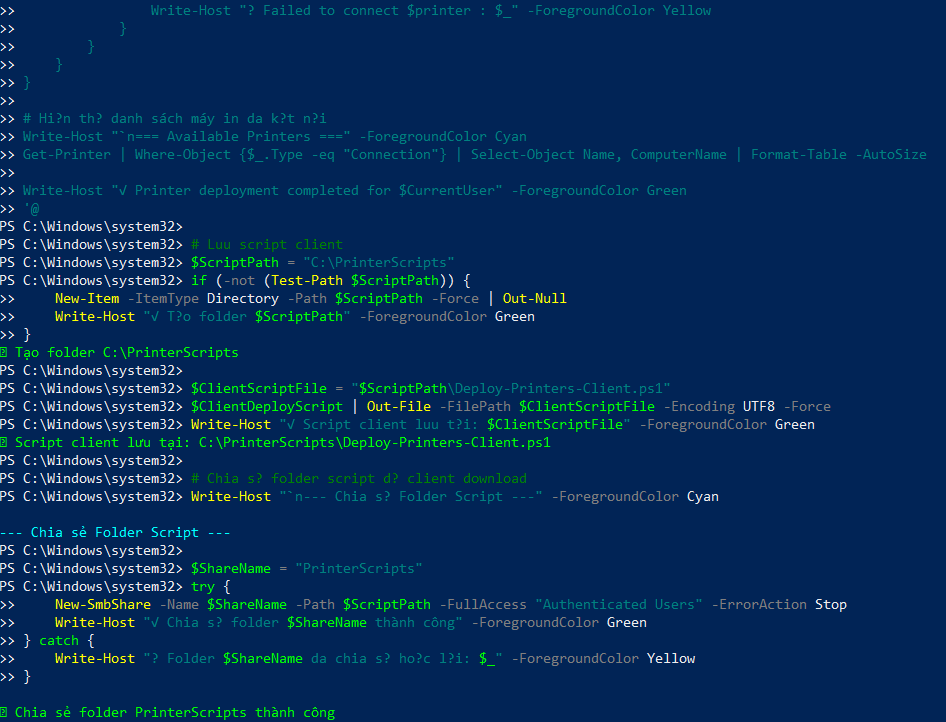
\includegraphics[width=0.7\textwidth]{./media/TẠO SCRIPT PHÂN PHỐI MÁY IN ĐẾN CLIENT(1).png}
    \vspace{-0.25cm}
    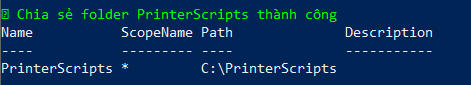
\includegraphics[width=0.7\textwidth]{./media/TẠO SCRIPT PHÂN PHỐI MÁY IN ĐẾN CLIENT(2).png}
    \caption{Tạo script phân phối máy in đến client}
    \label{fig:mirrored_vd_17}
\end{figure}

\section{Gán Script qua GPO}
\begin{lstlisting}[style=powershell]
$DomainDN = "DC=ABC,DC=local"
 
Write-Host "=== Create Department OUs ===" -ForegroundColor Cyan
 
# Create Parent OU
try {
    New-ADOrganizationalUnit -Name "PrinterGroups" -Path "OU=PrinterManagement,$DomainDN" -ProtectedFromAccidentalDeletion $false -ErrorAction SilentlyContinue
    Write-Host "[OK] OU PrinterGroups created successfully" -ForegroundColor Green
} catch {
    Write-Host "[!] OU PrinterGroups error: $_" -ForegroundColor Yellow
}
 
# Create Child OUs for each department
$DeptOUs = @(
    @{Name="Design"; Path="OU=PrinterGroups,OU=PrinterManagement,$DomainDN"},
    @{Name="Office"; Path="OU=PrinterGroups,OU=PrinterManagement,$DomainDN"},
    @{Name="Accounting"; Path="OU=PrinterGroups,OU=PrinterManagement,$DomainDN"}
)
 
foreach ($deptou in $DeptOUs) {
    try {
        New-ADOrganizationalUnit -Name $deptou.Name -Path $deptou.Path -ProtectedFromAccidentalDeletion $false -ErrorAction Stop
        Write-Host "[OK] OU '$($deptou.Name)' created successfully" -ForegroundColor Green
    } catch {
        Write-Host "[!] OU '$($deptou.Name)' error: $_" -ForegroundColor Yellow
    }
}
 
Start-Sleep -Seconds 2
 
# Link GPO to OU
Write-Host "`n=== Link GPO to OU ===" -ForegroundColor Cyan
 
$GPOConfigs = @(
    @{Name="Printers_Design"; Target="OU=Design,OU=PrinterGroups,OU=PrinterManagement,DC=ABC,DC=local"},
    @{Name="Printers_Office"; Target="OU=Office,OU=PrinterGroups,OU=PrinterManagement,DC=ABC,DC=local"},
    @{Name="Printers_Accounting"; Target="OU=Accounting,OU=PrinterGroups,OU=PrinterManagement,DC=ABC,DC=local"}
)
 
foreach ($gpo in $GPOConfigs) {
    try {
        # Note: The GPO must exist before linking
        New-GPLink -Name $gpo.Name -Target $gpo.Target -LinkEnabled Yes -ErrorAction Stop
        Write-Host "[OK] Linked GPO '$($gpo.Name)' successfully" -ForegroundColor Green
    } catch {
        Write-Host "[!] Error linking '$($gpo.Name)': $_" -ForegroundColor Yellow
    }
}
\end{lstlisting}

\begin{figure}[htbp]
    \centering
    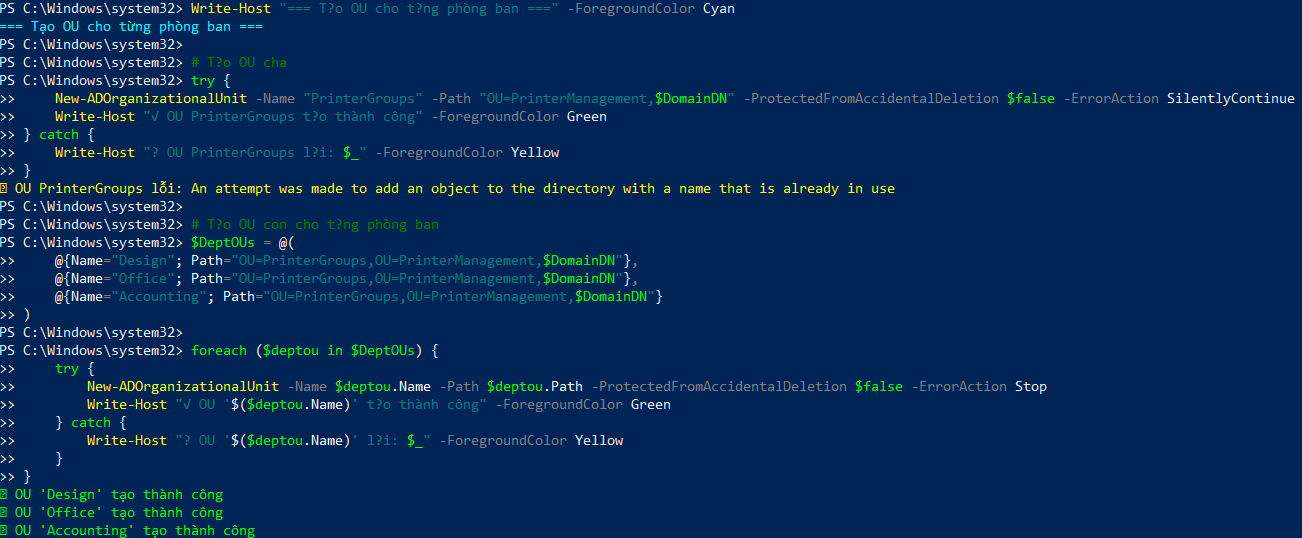
\includegraphics[width=0.68\textwidth]{./media/TẠO GROUP POLICY OBJECT (GPO) ĐỂ PHÂN PHỐI MÁY IN.png}
    \vspace{-0.2cm}
    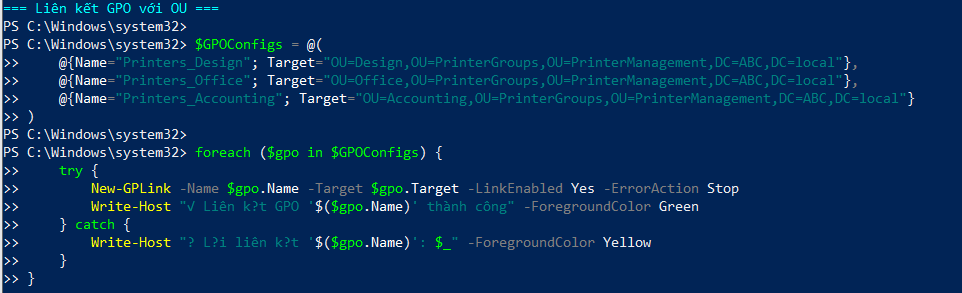
\includegraphics[width=0.68\textwidth]{./media/TẠO GROUP POLICY OBJECT (GPO) ĐỂ PHÂN PHỐI MÁY IN(1).png}
    \vspace{-0.2cm}
    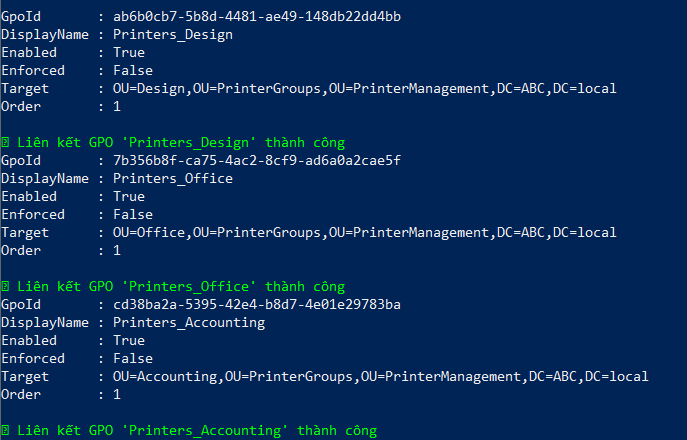
\includegraphics[width=0.68\textwidth]{./media/TẠO GROUP POLICY OBJECT (GPO) ĐỂ PHÂN PHỐI MÁY IN(2).png}
    \vspace{-0.2cm}
    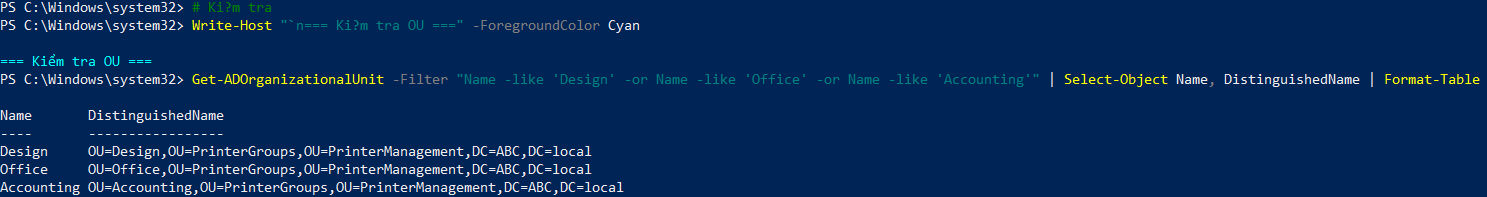
\includegraphics[width=0.68\textwidth]{./media/TẠO GROUP POLICY OBJECT (GPO) ĐỂ PHÂN PHỐI MÁY IN(3).png}
    \vspace{-0.2cm}
    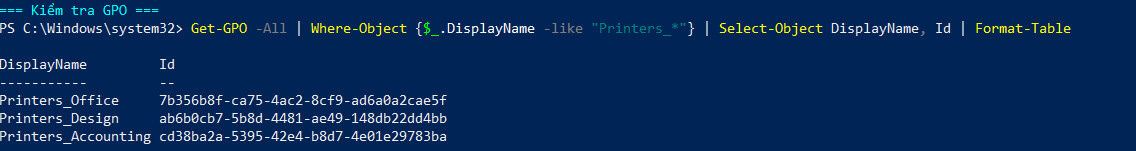
\includegraphics[width=0.68\textwidth]{./media/TẠO GROUP POLICY OBJECT (GPO) ĐỂ PHÂN PHỐI MÁY IN(4).png}
    \caption{Tạo Group Policy Object (GPO) để phân phối máy in}
    \label{fig:mirrored_vd_13}
\end{figure}

\subsection{Tạo script đọc group của user hiện tại bằng .NET}
\begin{lstlisting}[style=powershell]
$SysvolScriptPath = "C:\Windows\SYSVOL\sysvol\ABC.local\scripts\Map-DeptPrinters.ps1"
 
@'
# Map printers by department groups without AD module
 
$identity = [System.Security.Principal.WindowsIdentity]::GetCurrent()
$groups = @()
foreach ($g in $identity.Groups) {
    try {
        $name = $g.Translate([System.Security.Principal.NTAccount]).Value
        if ($name) { $groups += $name }
    } catch { }
}
 
function In-Group {
    param([string]$GroupName)
    return $groups -like "*\$GroupName"
}
 
# Debug
Write-Host "User: $($identity.Name)"
Write-Host "Groups:"; $groups | ForEach-Object { Write-Host "   $_" }
 
if (In-Group "GRP_Design") {
    Write-Host "User is in GRP_Design, mapping Design printers..."
    Add-Printer -ConnectionName "\\SRV-PRINT\PRN_Design_01" -ErrorAction SilentlyContinue
    Add-Printer -ConnectionName "\\SRV-PRINT\PRN_Design_02" -ErrorAction SilentlyContinue
}
 
if (In-Group "GRP_Office") {
    Write-Host "User is in GRP_Office, mapping Office printers..."
    Add-Printer -ConnectionName "\\SRV-PRINT\PRN_Office_01" -ErrorAction SilentlyContinue
    Add-Printer -ConnectionName "\\SRV-PRINT\PRN_Office_02" -ErrorAction SilentlyContinue
    Add-Printer -ConnectionName "\\SRV-PRINT\PRN_Office_03" -ErrorAction SilentlyContinue
    Add-Printer -ConnectionName "\\SRV-PRINT\PRN_Pool_Office" -ErrorAction SilentlyContinue
}
 
if (In-Group "GRP_Accounting") {
    Write-Host "User is in GRP_Accounting, mapping Accounting printers..."
    Add-Printer -ConnectionName "\\SRV-PRINT\PRN_Accounting_01" -ErrorAction SilentlyContinue
    Add-Printer -ConnectionName "\\SRV-PRINT\PRN_Accounting_02" -ErrorAction SilentlyContinue
}
'@ | Set-Content -Path $SysvolScriptPath -Encoding ASCII
\end{lstlisting}

\begin{figure}[htbp]
    \centering
    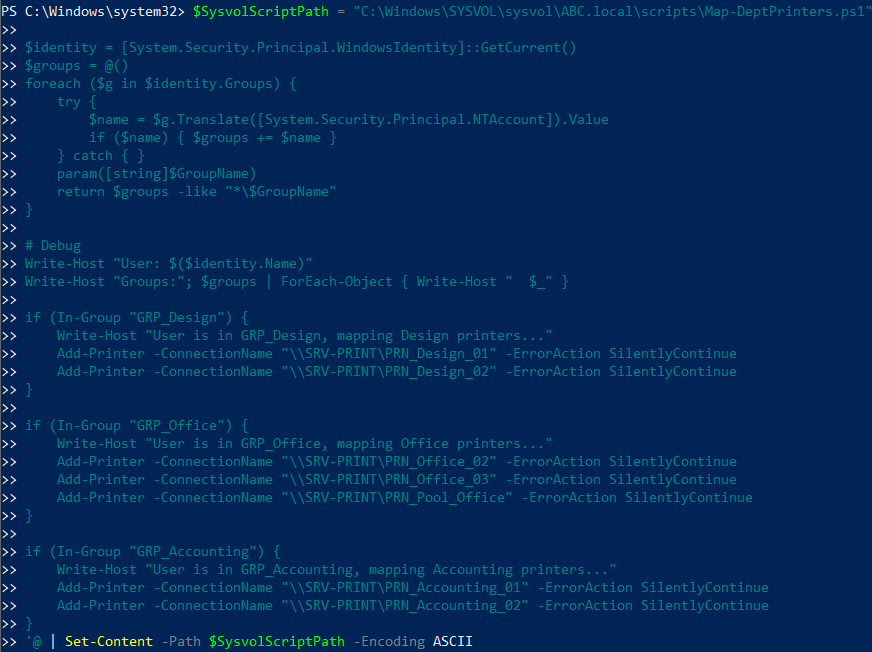
\includegraphics[width=0.75\textwidth]{./media/Tạo script đọc group của user hiện tại bằng .NET.png}
    \caption{Tạo script đọc group của user hiện tại bằng .NET}
    \label{fig:mirrored_vd_14}
\end{figure}

\subsection{Tạo GPO để chạy script khi user logon}
\begin{lstlisting}[style=powershell]
New-GPO -Name "GPO_PrinterDeploy" | Out-Null

New-GPLink -Name "GPO_PrinterDeploy" -Target "OU=Users,OU=PrinterManagement,DC=ABC,DC=local" -LinkEnabled Yes

Set-GPRegistryValue `
  -Name "GPO_PrinterDeploy" `
  -Key "HKCU\Software\Microsoft\Windows\CurrentVersion\Run" `
  -ValueName "MapPrinters" `
  -Type String `
  -Value "powershell.exe -ExecutionPolicy Bypass -File \\SRV-PRINT\sysvol\ABC.local\scripts\Map-DeptPrinters.ps1"
\end{lstlisting}

\begin{figure}[htbp]
    \centering
    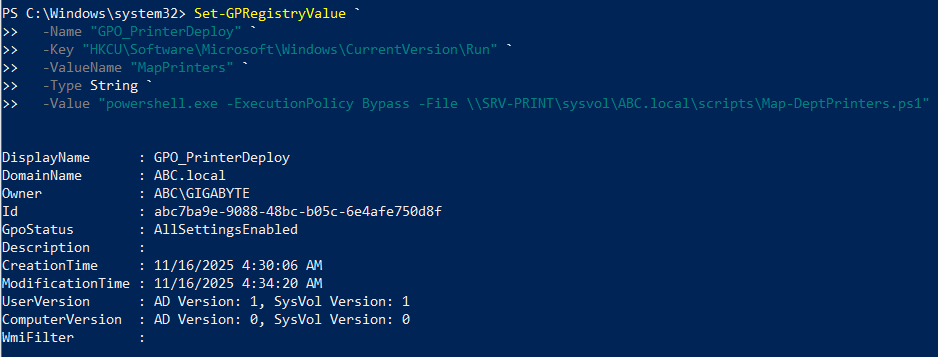
\includegraphics[width=0.75\textwidth]{./media/Tạo 1 GPO duy nhất để chạy script này khi user logon.png}
    \caption{Tạo GPO để chạy script khi user logon}
    \label{fig:mirrored_vd_115}
\end{figure}

\chapter{\textbf{Cấu hình Client tham gia Domain}}
\section{Join Domain trên Client PowerShell (As Administrator)}
Trên mỗi máy Client chạy lệnh:
\begin{lstlisting}[style=powershell]
# Dat DNS chi ve Domain Controller
$Adapter = Get-NetAdapter | Where-Object {$_.Status -eq "Up"} | Select-Object -First 1
Set-DnsClientServerAddress -InterfaceAlias $Adapter.Name -ServerAddresses "192.168.244.10"

# Join domain
$SecurePassword = ConvertTo-SecureString "ADMIN_PASSWORD" -AsPlainText -Force
$Credential = New-Object System.Management.Automation.PSCredential("abc\Administrator", $SecurePassword)
Add-Computer -DomainName "abc.local" -Credential $Credential -Force -Restart

Write-Host "Client tham gia domain thanh cong" -ForegroundColor Green
\end{lstlisting}

\subsection{Đăng nhập với Account Test}
Sau khi restart, đăng nhập với các tài khoản sau:
\begin{itemize}[topsep=2pt,itemsep=1pt,parsep=0pt]
    \item \textbf{User 1 (Phòng Thiết kế):} \texttt{ABC\textbackslash user\_design}
    \item \textbf{User 2 (Phòng Văn phòng):} \texttt{ABC\textbackslash user\_office}
    \item \textbf{User 3 (Phòng Kế toán):} \texttt{ABC\textbackslash user\_accounting}
\end{itemize}
\textbf{Password:} \texttt{Manh31102005}

\section{Kiểm tra máy in được map tự động}
Sau khi đăng nhập vào \texttt{ABC\textbackslash user\_office} với password \texttt{Manh31102005}, chạy các lệnh sau:
\begin{lstlisting}[style=powershell]
# Cho phep chay script trong phien hien tai
Set-ExecutionPolicy -Scope Process -ExecutionPolicy Bypass -Force
whoami /groups | findstr /i grp
Get-Printer | Format-Table Name,ShareName
\end{lstlisting}

\begin{figure}[htbp]
    \centering
    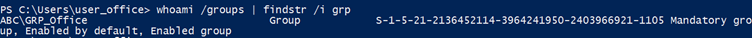
\includegraphics[width=0.75\textwidth]{./media/1.png}
    \vspace{-0.25cm}
    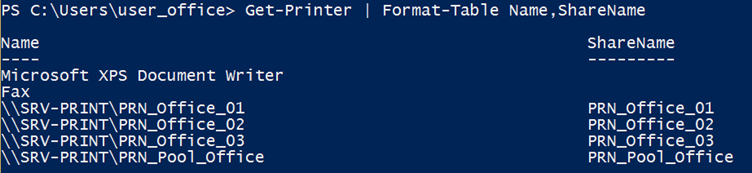
\includegraphics[width=0.75\textwidth]{./media/2.png}
    \caption{Kết quả kiểm tra sau khi đăng nhập}
    \label{fig:login_check}
\end{figure}

\subsection{Thực hiện test in}
\textbf{Bước 1:} Mở Notepad trên client

\textbf{Bước 2:} Gõ nội dung: \texttt{Test Print - user\_office}

\textbf{Bước 3:} Thực hiện in:
\begin{itemize}[topsep=2pt,itemsep=1pt,parsep=0pt]
    \item Chọn \texttt{File → Print}
    \item Chọn máy in: \texttt{\textbackslash\textbackslash SRV-PRINT\textbackslash PRN\_Office\_01}
    \item Nhấn \texttt{Print}
\end{itemize}

\textbf{Bước 4:} Kiểm tra print job:
\begin{lstlisting}[style=powershell]
Get-WmiObject -Class Win32_PrintJob |
    Select-Object Name, Document, JobId, Owner, TotalPages, Status | Format-Table -AutoSize
\end{lstlisting}

\begin{figure}[htbp]
    \centering
    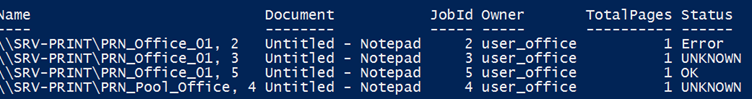
\includegraphics[width=0.8\textwidth]{./media/3.png}
    \caption{Kết quả kiểm tra print job}
    \label{fig:print_job}
\end{figure}

\subsection{Kiểm tra queue trên Server}
\begin{lstlisting}[style=powershell]
Get-PrintJob -PrinterName "PRN_Office_01" |
    Select PrinterName, JobId, JobStatus, Owner, DocumentName, SubmittedTime |
    Format-Table -AutoSize
\end{lstlisting}

\begin{figure}[htbp]
    \centering
    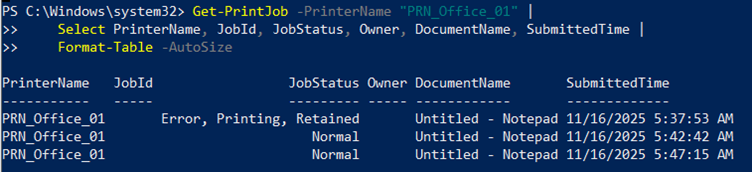
\includegraphics[width=0.8\textwidth]{./media/4.png}
    \caption{Kiểm tra queue trên server}
    \label{fig:server_queue}
\end{figure}

\subsection{Kiểm tra Event Log}
\begin{lstlisting}[style=powershell]
Get-EventLog -LogName "Print Service Log" -Newest 20
\end{lstlisting}

\begin{figure}[htbp]
    \centering
    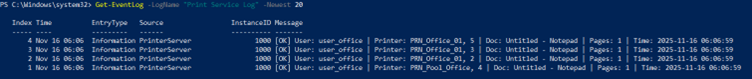
\includegraphics[width=0.8\textwidth]{./media/5.png}
    \caption{Event log của Print Service}
    \label{fig:event_log}
\end{figure}
\vspace{\baselineskip}

\chapter{\textbf{Giám sát, logging và báo cáo}}
\section{Bật Logging PrintService}
\begin{lstlisting}[style=powershell]
# Create Custom Event Log
try {
    New-EventLog -LogName "Print Service Log" -Source "PrinterServer" -ErrorAction SilentlyContinue
    Write-Host "[OK] Event Log 'Print Service Log' created successfully" -ForegroundColor Green
} catch {
    Write-Host "[!] Event Log already exists or error: $_" -ForegroundColor Yellow
}
 
# Create folder to save log files
$LogFolder = "C:\PrintLogs"
if (-not (Test-Path $LogFolder)) {
    New-Item -ItemType Directory -Path $LogFolder -Force | Out-Null
    Write-Host "[OK] Folder $LogFolder created successfully" -ForegroundColor Green
} else {
    Write-Host "[OK] Folder $LogFolder already exists" -ForegroundColor Green
}
 
# Function to log details of every print job
Function Log-PrintEvent {
    param(
        [string]$Username,
        [string]$PrinterName,
        [string]$DocumentName,
        [int]$PageCount,
        [string]$EventType = "Print Job Submitted",
        [string]$Status = "Success"
    )
    
    $Timestamp = Get-Date -Format "yyyy-MM-dd HH:mm:ss"
    
    # Write to Event Log
    try {
        Write-EventLog -LogName "Print Service Log" `
                      -Source "PrinterServer" `
                      -EventId 1000 `
                      -EntryType Information `
                      -Message "[$Status] User: $Username | Printer: $PrinterName | Doc: $DocumentName | Pages: $PageCount | Time: $Timestamp"
    } catch {
        Write-Host "[!] Error writing to Event Log: $_" -ForegroundColor Yellow
    }
    
    # Write to CSV file for long-term storage
    $CSVPath = "$LogFolder\PrintHistory.csv"
    $LogEntry = [PSCustomObject]@{
        Timestamp = $Timestamp
        Username = $Username
        PrinterName = $PrinterName
        DocumentName = $DocumentName
        PageCount = $PageCount
        EventType = $EventType
        Status = $Status
    }
    
    try {
        $LogEntry | Export-Csv -Path $CSVPath -Append -NoTypeInformation -Force -ErrorAction Stop
    } catch {
        Write-Host "[!] Error writing to CSV log: $_" -ForegroundColor Yellow
    }
}
 
Write-Host "[OK] Function Log-PrintEvent created" -ForegroundColor Green
\end{lstlisting}

\begin{figure}[htbp]
    \centering
    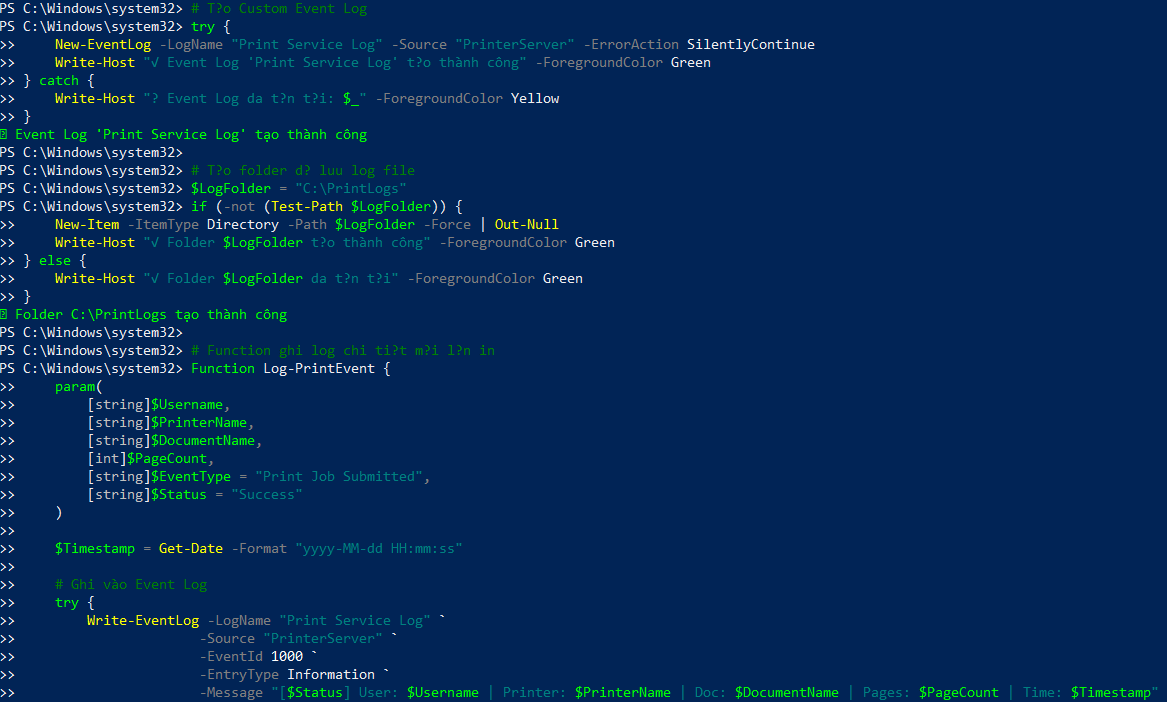
\includegraphics[width=0.72\textwidth]{./media/CẤU HÌNH LOGGING CHI TIẾT.png}
    \vspace{-0.25cm}
    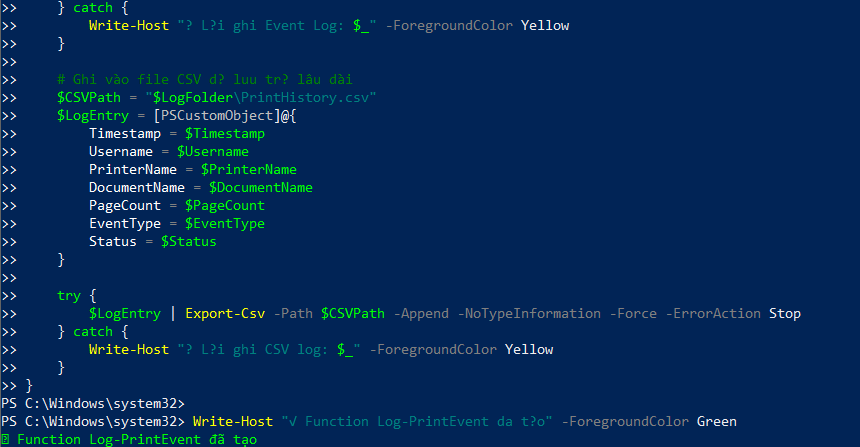
\includegraphics[width=0.72\textwidth]{./media/CẤU HÌNH LOGGING CHI TIẾT(1).png}
    \caption{Cấu hình logging chi tiết}
    \label{fig:mirrored_vd_10}
\end{figure}

\subsection{Script kiểm tra Log event}
\begin{lstlisting}[style=powershell]
# List of logged jobs (to avoid duplicates)
$global:LoggedJobs = @{}
 
# 3-second Timer
$timer = New-Object Timers.Timer
$timer.Interval = 3000
$timer.AutoReset = $true
$timer.Enabled = $true
 
Register-ObjectEvent `
    -InputObject $timer `
    -EventName Elapsed `
    -SourceIdentifier "PrintJobMonitor" `
    -Action {
 
        $jobs = Get-WmiObject -Class Win32_PrintJob -ErrorAction SilentlyContinue
 
        foreach ($job in $jobs) {
 
            # Each job has JobID + PrinterName to create a unique key
            $key = "$($job.Name)-$($job.JobId)"
 
            # If this job hasn't been logged yet -> log immediately
            if (-not $global:LoggedJobs.ContainsKey($key)) {
 
                $global:LoggedJobs[$key] = $true
 
                # Call the logging function defined previously
                Log-PrintEvent `
                    -Username $job.Owner `
                    -PrinterName $job.Name `
                    -DocumentName $job.Document `
                    -PageCount $job.TotalPages `
                    -EventType "Print Job" `
                    -Status "OK"
 
                Write-Host "Logged: $key" -ForegroundColor Green
            }
        }
    }
\end{lstlisting}

\begin{figure}[htbp]
    \centering
    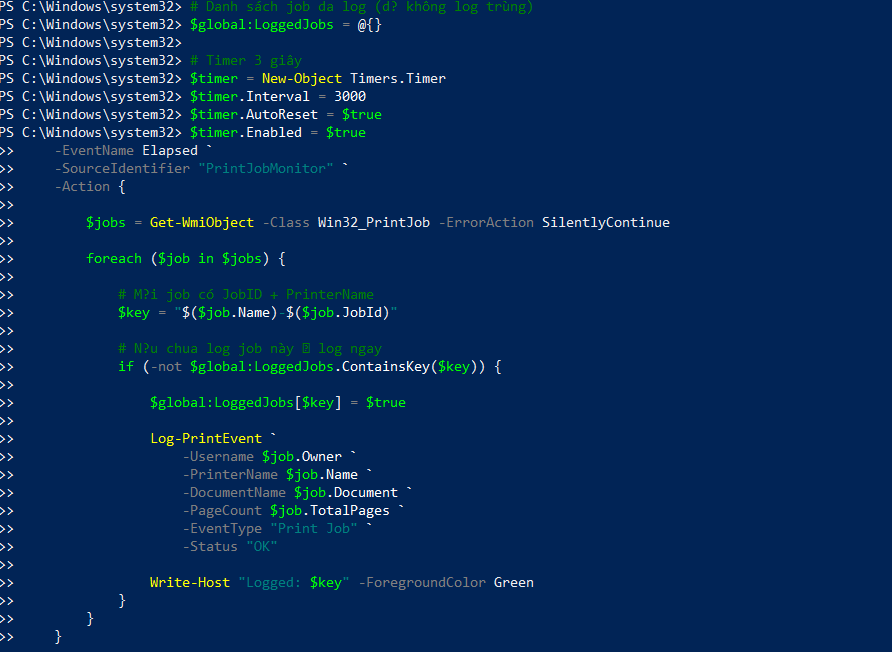
\includegraphics[width=0.99\textwidth]{./media/kiểm tra Log event.png}
    \vspace{-0.25cm}
    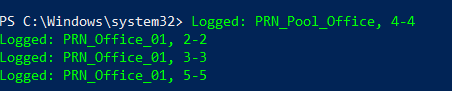
\includegraphics[width=0.99\textwidth]{./media/kiểm tra Log event(1).png}
    \caption{Kiểm tra Log event}
    \label{fig:mirrored_vd_11}
\end{figure}
\clearpage

\section{Thống kê theo người dùng và Xuất báo cáo bằng PowerShell}
\begin{lstlisting}[style=powershell]
Function Get-PrinterUsageReport {
    param(
        [string]$Username = $null,
        [DateTime]$StartDate = (Get-Date).AddDays(-30),
        [DateTime]$EndDate = (Get-Date)
    )
    
    $CSVPath = "$LogFolder\PrintHistory.csv"
    
    if (-not (Test-Path $CSVPath)) {
        Write-Host "[!] Log file not found: $CSVPath" -ForegroundColor Yellow
        return $null
    }
    
    # Read log file
    $PrintLog = Import-Csv -Path $CSVPath -ErrorAction SilentlyContinue
    if (-not $PrintLog) {
        Write-Host "[!] Log file is empty" -ForegroundColor Yellow
        return $null
    }
    
    # Filter by user and date
    $FilteredLog = $PrintLog | Where-Object {
        $LogDate = $null
        if ([DateTime]::TryParseExact($_.Timestamp, "yyyy-MM-dd HH:mm:ss", $null, [System.Globalization.DateTimeStyles]::None, [ref]$LogDate)) {
            ($null -eq $Username -or $_.Username -eq $Username) -and
            ($LogDate -ge $StartDate -and $LogDate -le $EndDate)
        }
    }
    
    if (-not $FilteredLog) {
        Write-Host "[!] No data found for the selected date range" -ForegroundColor Yellow
        return $null
    }
    
    # Calculate statistics
    $Report = $FilteredLog | Group-Object -Property Username | ForEach-Object {
        $Pages = $_.Group.PageCount | Measure-Object -Sum
        [PSCustomObject]@{
            Username = $_.Name
            TotalJobs = $_.Count
            TotalPages = $Pages.Sum
            AveragePagesPerJob = [Math]::Round($Pages.Sum / $_.Count, 2)
            MostUsedPrinter = ($_.Group | Group-Object -Property PrinterName | Sort-Object Count -Descending | Select-Object -First 1).Name
            FirstJobTime = ($_.Group | Sort-Object Timestamp | Select-Object -First 1).Timestamp
            LastJobTime = ($_.Group | Sort-Object Timestamp | Select-Object -Last 1).Timestamp
        }
    }
    
    return $Report
}
 
Function Export-PrinterReportToCSV {
    param(
        [string]$OutputPath = "$LogFolder\Report_$(Get-Date -Format 'yyyy-MM-dd_HH-mm-ss').csv",
        [int]$DaysBack = 30
    )
    
    Write-Host "Generating report for last $DaysBack days..." -ForegroundColor Cyan
    
    $StartDate = (Get-Date).AddDays(-$DaysBack)
    $Report = Get-PrinterUsageReport -StartDate $StartDate
    
    if ($Report) {
        $Report | Export-Csv -Path $OutputPath -NoTypeInformation -Force
        Write-Host "[OK] Report exported: $OutputPath" -ForegroundColor Green
        $Report | Format-Table -AutoSize
    } else {
        Write-Host "[!] No data available to export report" -ForegroundColor Yellow
    }
}
 
Function Export-UserPrinterHistory {
    param(
        [Parameter(Mandatory=$true)][string]$Username,
        [string]$OutputPath = "$LogFolder\History_$($Username)_$(Get-Date -Format 'yyyy-MM-dd_HH-mm-ss').csv"
    )
    
    Write-Host "Exporting history for user: $Username" -ForegroundColor Cyan
    
    $CSVPath = "$LogFolder\PrintHistory.csv"
    if (-not (Test-Path $CSVPath)) {
        Write-Host "[!] Log file not found" -ForegroundColor Yellow
        return
    }
    
    $PrintLog = Import-Csv -Path $CSVPath
    $UserHistory = $PrintLog | Where-Object {$_.Username -eq $Username}
    
    if ($UserHistory) {
        $UserHistory | Export-Csv -Path $OutputPath -NoTypeInformation -Force
        Write-Host "[OK] Print history for $Username exported: $OutputPath" -ForegroundColor Green
        $UserHistory | Format-Table -AutoSize
    } else {
        Write-Host "[!] No data found for user $Username" -ForegroundColor Yellow
    }
}
 
Write-Host "[OK] Report functions created" -ForegroundColor Green
\end{lstlisting}
% \begin{figure}[htbp]
%     \centering
%     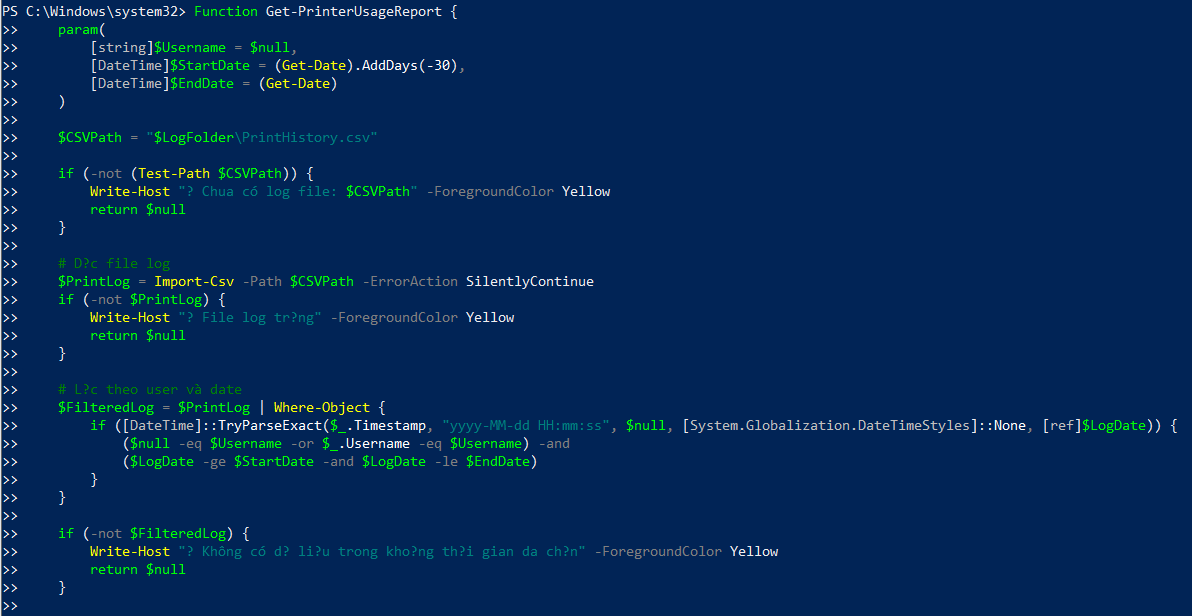
\includegraphics[width=0.68\textwidth]{./media/HÀM THỐNG KÊ VÀ XUẤT BÁO CÁO.png}
%     \vspace{-0.2cm}
%     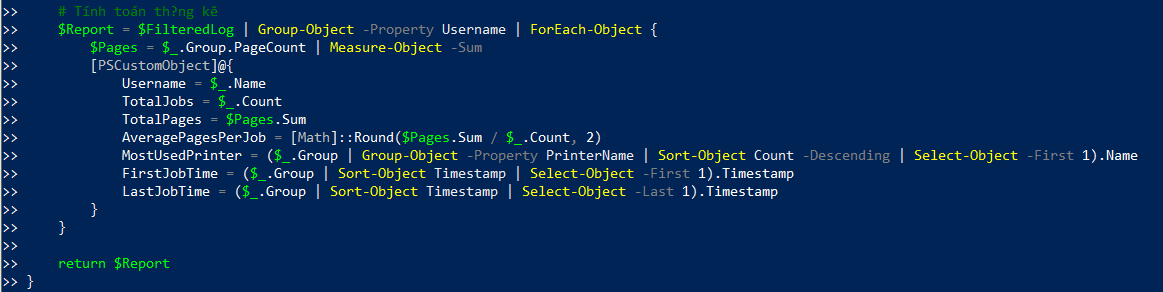
\includegraphics[width=0.68\textwidth]{./media/HÀM THỐNG KÊ VÀ XUẤT BÁO CÁO(1).png}
%     \label{fig:mirrored_vd_18}
% \end{figure}
\begin{figure}[htbp]
    \centering
    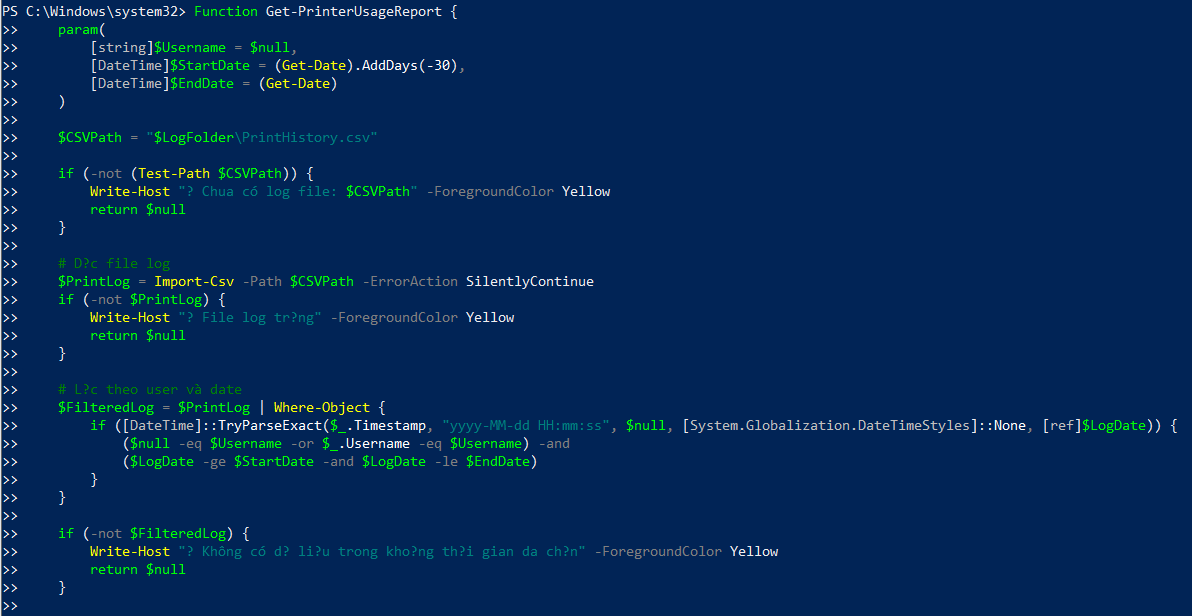
\includegraphics[width=0.68\textwidth]{./media/HÀM THỐNG KÊ VÀ XUẤT BÁO CÁO.png}
    \vspace{-0.2cm}
    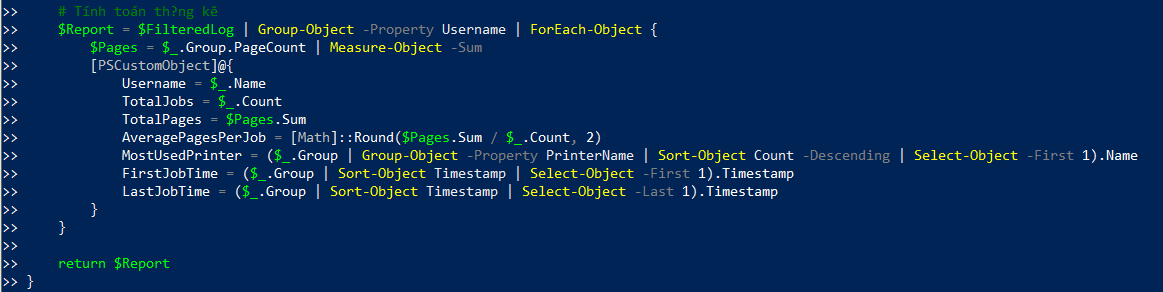
\includegraphics[width=0.68\textwidth]{./media/HÀM THỐNG KÊ VÀ XUẤT BÁO CÁO(1).png}
    \vspace{-0.2cm}
    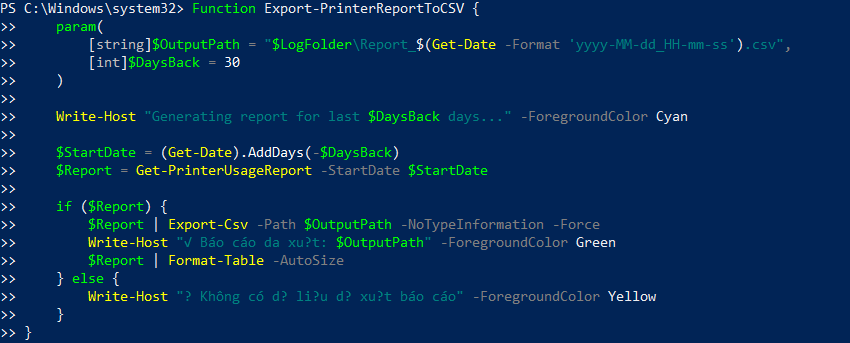
\includegraphics[width=0.68\textwidth]{./media/HÀM THỐNG KÊ VÀ XUẤT BÁO CÁO(2).png}
    \vspace{-0.2cm}
    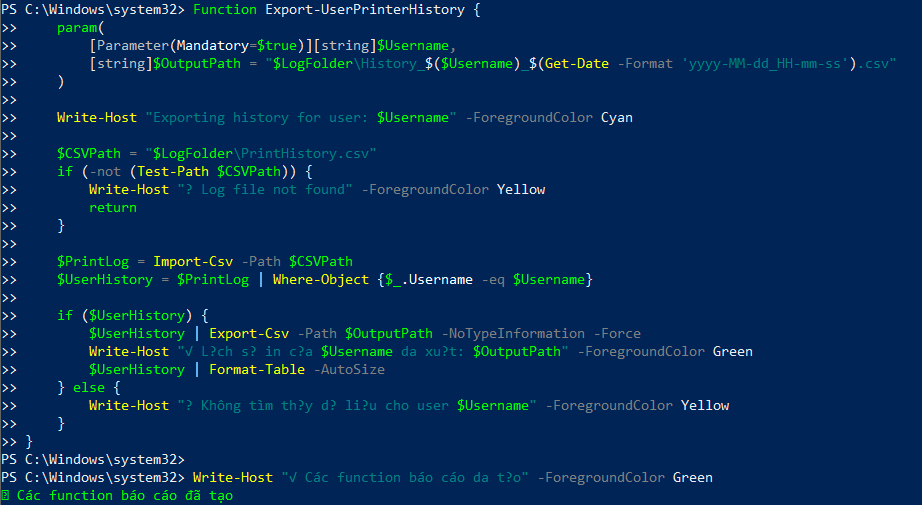
\includegraphics[width=0.68\textwidth]{./media/HÀM THỐNG KÊ VÀ XUẤT BÁO CÁO(3).png}
    \caption{Thống kê và xuất báo cáo}
    \label{fig:mirrored_vd_18}
\end{figure}
\vspace{\baselineskip}
\clearpage
\chapter{\textbf{Kiểm thử và xác thực hệ thống}}
\section{Giới thiệu}
Phần này cung cấp script tổng hợp để kiểm tra và đánh giá tình trạng hoạt động của toàn bộ hệ thống Print Server. Script thực hiện quét tuần tự qua 9 thành phần chính của hệ thống, từ cấp độ Domain Controller đến các dịch vụ và logging, giúp quản trị viên có cái nhìn toàn diện về tình trạng hệ thống trong một lần chạy.

\section{Các thành phần kiểm tra}

\subsection{Kiểm tra Domain}
Xác minh kết nối đến Active Directory Forest, hiển thị tên domain và mức độ chức năng (Forest Mode). Đây là bước đầu tiên để đảm bảo hạ tầng AD hoạt động bình thường.

\begin{lstlisting}[style=powershell]
Write-Host "`n--- 1. Kiem tra Domain ---" -ForegroundColor Cyan
try {
    $Forest = Get-ADForest -ErrorAction Stop
    Write-Host "Forest: $($Forest.Name)" -ForegroundColor Green
    Write-Host "Domain Level: $($Forest.ForestMode)" -ForegroundColor Green
} catch {
    Write-Host "Loi: $_" -ForegroundColor Red
}
\end{lstlisting}

\subsection{Kiểm tra Nhóm AD}
Liệt kê tất cả các nhóm có tiền tố "GRP\_" và đếm số lượng thành viên trong mỗi nhóm. Giúp xác nhận cấu trúc phân quyền theo phòng ban đã được triển khai đúng.

\begin{lstlisting}[style=powershell]
Write-Host "`n--- 2. Kiem tra Nhom AD ---" -ForegroundColor Cyan
$Groups = Get-ADGroup -Filter "Name -like 'GRP_*'" -ErrorAction SilentlyContinue
foreach ($group in $Groups) {
    $members = Get-ADGroupMember -Identity $group.Name -ErrorAction SilentlyContinue
    Write-Host "Nhom: $($group.Name) - Members: $($members.Count)" -ForegroundColor Green
}
\end{lstlisting}

\subsection{Kiểm tra User}
Hiển thị danh sách người dùng có tên đăng nhập bắt đầu bằng "user\_" kèm theo tên hiển thị. Xác nhận các tài khoản người dùng đã được tạo và cấu hình.

\begin{lstlisting}[style=powershell]
Write-Host "`n--- 3. Kiem tra User ---" -ForegroundColor Cyan
$Users = Get-ADUser -Filter "SamAccountName -like 'user_*'" -ErrorAction SilentlyContinue
foreach ($user in $Users) {
    Write-Host "User: $($user.SamAccountName) - $($user.DisplayName)" -ForegroundColor Green
}
\end{lstlisting}

\subsection{Kiểm tra Máy In}
Thống kê tổng số máy in trong hệ thống và số lượng máy in được chia sẻ. Đây là chỉ số quan trọng để đánh giá quy mô triển khai.

\begin{lstlisting}[style=powershell]
Write-Host "`n--- 4. Kiem tra May In ---" -ForegroundColor Cyan
$Printers = Get-Printer
Write-Host "Tong may in: $($Printers.Count)" -ForegroundColor Green
$SharedPrinters = $Printers | Where-Object {$_.Shared -eq $true}
Write-Host "May in chia se: $($SharedPrinters.Count)" -ForegroundColor Green
\end{lstlisting}

\subsection{Kiểm tra Cổng In}
Đếm số lượng cổng TCP/IP có tiền tố "IP\_", xác nhận các máy in network đã được cấu hình đúng địa chỉ.

\begin{lstlisting}[style=powershell]
Write-Host "`n--- 5. Kiem tra Cong In ---" -ForegroundColor Cyan
$Ports = Get-PrinterPort | Where-Object {$_.Name -like "IP_*"}
Write-Host "Cong in TCP/IP: $($Ports.Count)" -ForegroundColor Green
\end{lstlisting}

\subsection{Kiểm tra Printer Pool}
Xác minh máy in pool "PRN\_Pool\_Office" có tồn tại và được chia sẻ hay không. Đây là thành phần quan trọng cho việc cân bằng tải in ấn.

\begin{lstlisting}[style=powershell]
Write-Host "`n--- 6. Kiem tra Pool ---" -ForegroundColor Cyan
$PoolPrinter = Get-Printer -Name "PRN_Pool_Office" -ErrorAction SilentlyContinue
if ($PoolPrinter) {
    Write-Host "Pool: PRN_Pool_Office - Chia se: $($PoolPrinter.Shared)" -ForegroundColor Green
} else {
    Write-Host "Pool PRN_Pool_Office khong tim thay" -ForegroundColor Yellow
}
\end{lstlisting}

\subsection{Kiểm tra GPO}
Liệt kê tất cả Group Policy Objects có tên bắt đầu bằng "Printers\_" và hiển thị tên từng GPO. Xác nhận các chính sách triển khai máy in đã được tạo.

\begin{lstlisting}[style=powershell]
Write-Host "`n--- 7. Kiem tra GPO ---" -ForegroundColor Cyan
$GPOs = Get-GPO -All -ErrorAction SilentlyContinue | Where-Object {$_.DisplayName -like "Printers_*"}
Write-Host "Group Policies (Printer): $($GPOs.Count)" -ForegroundColor Green
foreach ($gpo in $GPOs) {
    Write-Host "  - $($gpo.DisplayName)" -ForegroundColor Cyan
}
\end{lstlisting}

\subsection{Kiểm tra Dịch vụ}
Kiểm tra trạng thái của 3 dịch vụ quan trọng là Print Spooler, DNS Server và Active Directory Domain Services. Hiển thị trạng thái Running hoặc Stopped với mã màu tương ứng.

\begin{lstlisting}[style=powershell]
Write-Host "`n--- 8. Kiem tra Dich vu ---" -ForegroundColor Cyan
$Services = @(
    @{Name="Spooler"; DisplayName="Print Spooler"},
    @{Name="DNS"; DisplayName="DNS Server"},
    @{Name="NTDS"; DisplayName="Active Directory Domain Services"}
)

foreach ($svc in $Services) {
    $Service = Get-Service -Name $svc.Name -ErrorAction SilentlyContinue
    if ($Service) {
        Write-Host "$($svc.DisplayName): $($Service.Status)" -ForegroundColor $(if ($Service.Status -eq "Running") {"Green"} else {"Yellow"})
    }
}
\end{lstlisting}

\subsection{Kiểm tra Logging}
Xác nhận thư mục lưu trữ log files có tồn tại và đếm số lượng file log đã được tạo. Hỗ trợ việc audit và troubleshooting sau này.

\begin{lstlisting}[style=powershell]
Write-Host "`n--- 9. Kiem tra Logging ---" -ForegroundColor Cyan
if (Test-Path $LogFolder) {
    Write-Host "Folder Logging: $LogFolder" -ForegroundColor Green
    $LogFiles = Get-ChildItem -Path $LogFolder -ErrorAction SilentlyContinue
    Write-Host "File logs: $($LogFiles.Count)" -ForegroundColor Green
} else {
    Write-Host "Folder Logging khong tim thay" -ForegroundColor Yellow
}
\end{lstlisting}

\begin{figure}[htbp]
    \centering
    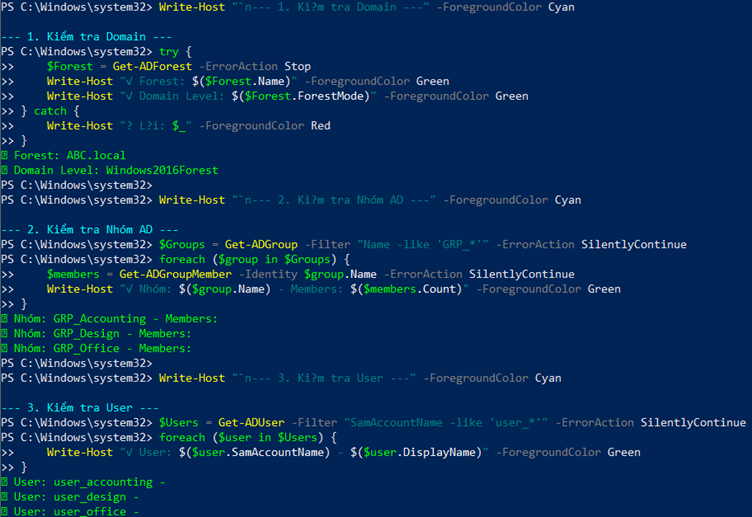
\includegraphics[width=0.65\textwidth]{./media/6.png}
    \vspace{-0.2cm}
    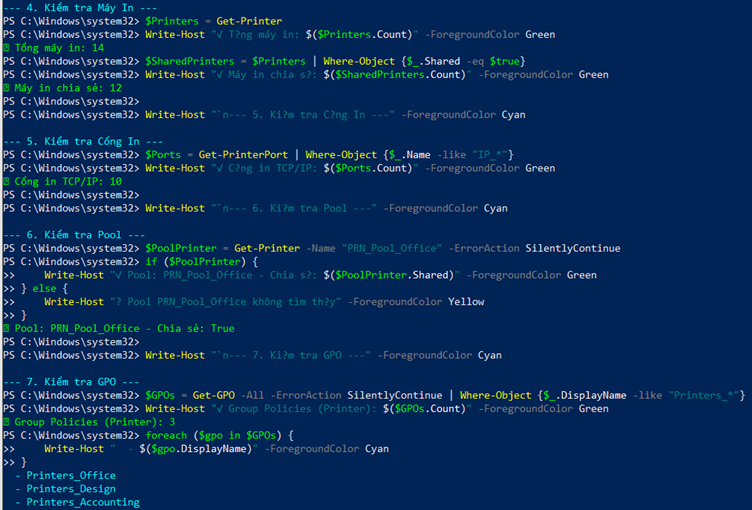
\includegraphics[width=0.65\textwidth]{./media/7.png}
    \vspace{-0.2cm}
    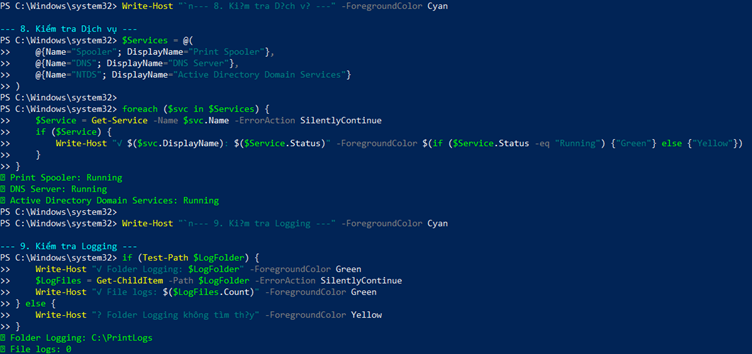
\includegraphics[width=0.65\textwidth]{./media/8.png}
    \caption{Kết quả sau khi kiểm tra}
    \label{fig:system_check}
\end{figure}

\section{Đặc điểm kỹ thuật}
Script sử dụng cơ chế xử lý lỗi (try-catch và -ErrorAction SilentlyContinue) để đảm bảo quá trình kiểm tra không bị gián đoạn khi gặp lỗi ở một thành phần. Mỗi mục kiểm tra được đánh số và có tiêu đề riêng với màu Cyan để dễ phân biệt. Kết quả hiển thị với hệ thống màu sắc: Green cho thành công, Yellow cho cảnh báo, và Red cho lỗi.

\section{Ứng dụng thực tế}
Script này được sử dụng làm công cụ kiểm tra tổng thể sau khi hoàn tất quá trình triển khai, hoặc để thực hiện health check định kỳ hàng tuần/hàng tháng. Quản trị viên có thể chạy script này để nhanh chóng đánh giá tình trạng hệ thống mà không cần kiểm tra từng thành phần riêng lẻ. Kết quả có thể được lưu lại làm báo cáo hoặc tài liệu tham khảo.

\section{Kết luận}
Phần kiểm tra toàn bộ hệ thống cung cấp một giải pháp tự động hóa cho việc đánh giá tổng thể Print Server infrastructure. Script giúp tiết kiệm thời gian, đảm bảo không bỏ sót thành phần nào và cung cấp báo cáo trực quan về tình trạng hệ thống trong thời gian thực.
\vspace{\baselineskip}

\chapter{\textbf{TROUBLESHOOTING \& GIẢI QUYẾT SỰ CỐ}}

\section{Giới thiệu}
Phần này cung cấp bộ công cụ PowerShell để kiểm tra, giám sát và xử lý sự cố cho hệ thống Print Server. Các function được thiết kế nhằm giúp quản trị viên nhanh chóng phát hiện và khắc phục các vấn đề thường gặp trong môi trường in ấn doanh nghiệp, đảm bảo hệ thống hoạt động ổn định và liên tục.

\section{Các chức năng chính}

\subsection{Get-PrinterServerStatus}
Function này kiểm tra tổng quan tình trạng Print Server bao gồm Domain Controller, các dịch vụ hệ thống (Spooler, DNS), thống kê số lượng máy in, cổng in, nhóm AD và GPO. Kết quả hiển thị dưới dạng bảng chi tiết với mã màu trực quan, giúp quản trị viên nhanh chóng nắm bắt tình trạng hoạt động của toàn bộ hệ thống và phát hiện các điểm bất thường.

\subsection{Clear-PrintQueue}
Xóa các công việc in bị treo trong hàng đợi, hỗ trợ xử lý cho một máy in cụ thể hoặc toàn bộ hệ thống. Đây là giải pháp nhanh và hiệu quả khi gặp tình trạng job in bị kẹt không thể xóa thủ công qua giao diện Windows. Function tự động đếm và báo cáo số lượng job đã được xóa thành công.

\subsection{Test-PrinterConnection}
Kiểm tra kết nối mạng đến một máy in cụ thể thông qua giao thức ICMP ping. Function này nhận vào địa chỉ IP và trả về trạng thái Online/Offline của thiết bị, giúp nhanh chóng xác định vấn đề kết nối mạng đến máy in đích.

\subsection{Test-AllPrinterConnections}
Tự động kiểm tra kết nối đến tất cả 10 máy in trong dải IP 192.168.244.201-210. Function này thực hiện ping tuần tự và hiển thị trạng thái của từng máy in, giúp quản trị viên nhanh chóng khảo sát tình trạng mạng của toàn bộ hệ thống máy in.

\subsection{Restart-PrintSpooler}
Khởi động lại dịch vụ Print Spooler với tùy chọn force để đảm bảo service được reset hoàn toàn. Đây là thao tác thường xuyên cần thiết khi máy in không nhận lệnh, hàng đợi bị treo, hoặc sau khi cài đặt driver mới. Function bao gồm xử lý lỗi để đảm bảo quá trình restart diễn ra an toàn.

\subsection{Get-PrinterDetailedInfo}
Hiển thị thông tin chi tiết về máy in (tên, máy chủ, trạng thái chia sẻ, cổng kết nối, mô tả, vị trí), cổng in (tên và địa chỉ IP), cùng với danh sách các công việc in đang chờ xử lý (người gửi, tài liệu, trạng thái, thời gian). Hỗ trợ hiệu quả cho việc troubleshooting chi tiết và audit hệ thống.

\section{Script tổng hợp}
\begin{lstlisting}[style=powershell]
Function Get-PrinterServerStatus {
    Write-Host "`n--- Trang thai Print Server ---" -ForegroundColor Cyan
    
    # Kiem tra domain controller
    try {
        $Forest = Get-ADForest -ErrorAction Stop
        Write-Host "Domain: $($Forest.Name)" -ForegroundColor Green
    } catch {
        Write-Host "Domain error: $_" -ForegroundColor Red
    }
    
    # Kiem tra dich vu Spooler
    $SpoolerStatus = Get-Service -Name Spooler -ErrorAction SilentlyContinue
    if ($SpoolerStatus.Status -eq "Running") {
        Write-Host "Print Spooler: Running" -ForegroundColor Green
    } else {
        Write-Host "Print Spooler: $($SpoolerStatus.Status)" -ForegroundColor Red
    }
    
    # Kiem tra DNS
    $DNSService = Get-Service -Name DNS -ErrorAction SilentlyContinue
    if ($DNSService.Status -eq "Running") {
        Write-Host "DNS Server: Running" -ForegroundColor Green
    } else {
        Write-Host "DNS Server: $($DNSService.Status)" -ForegroundColor Red
    }
    
    # Dem may in
    $SharedPrinters = @(Get-Printer | Where-Object {$_.Shared -eq $true})
    Write-Host "May in chia se: $($SharedPrinters.Count)" -ForegroundColor Green
    
    # Dem cong in
    $Ports = @(Get-PrinterPort | Where-Object {$_.Name -like "IP_*"})
    Write-Host "Cong in TCP/IP: $($Ports.Count)" -ForegroundColor Green
    
    # Kiem tra nhom AD
    $ADGroups = @(Get-ADGroup -Filter "Name -like 'GRP_*'" -ErrorAction SilentlyContinue)
    Write-Host "Nhom AD: $($ADGroups.Count)" -ForegroundColor Green
    
    # Kiem tra GPO
    $GPOs = @(Get-GPO -All -ErrorAction SilentlyContinue | Where-Object {$_.DisplayName -like "Printers_*"})
    Write-Host "Group Policies: $($GPOs.Count)" -ForegroundColor Green
    
    Write-Host "`n--- Chi tiet May In ---" -ForegroundColor Cyan
    Get-Printer | Select-Object Name, ComputerName, Shared, PortName | Format-Table -AutoSize
}

Function Clear-PrintQueue {
    param(
        [string]$PrinterName = $null
    )
    
    if ($PrinterName) {
        try {
            $Jobs = Get-PrintJob -PrinterName $PrinterName -ErrorAction Stop
            $Jobs | Remove-PrintJob -ErrorAction Stop
            Write-Host "Xoa $($Jobs.Count) cong viec khoi queue $PrinterName" -ForegroundColor Green
        } catch {
            Write-Host "Loi xoa queue: $_" -ForegroundColor Yellow
        }
    } else {
        try {
            $AllJobs = Get-PrintJob -ErrorAction Stop
            $AllJobs | Remove-PrintJob -ErrorAction Stop
            Write-Host "Xoa $($AllJobs.Count) cong viec tu tat ca may in" -ForegroundColor Green
        } catch {
            Write-Host "Loi xoa queue: $_" -ForegroundColor Yellow
        }
    }
}

Function Test-PrinterConnection {
    param(
        [string]$PrinterIP
    )
    
    $PingResult = Test-Connection -ComputerName $PrinterIP -Count 1 -Quiet -ErrorAction SilentlyContinue
    if ($PingResult) {
        Write-Host "May in ${PrinterIP}: Online" -ForegroundColor Green
    } else {
        Write-Host "May in ${PrinterIP}: Offline" -ForegroundColor Red
    }
}

Function Test-AllPrinterConnections {
    Write-Host "`n=== Testing All Printer Connections ===" -ForegroundColor Cyan
    $IPs = 201..210 | ForEach-Object {"192.168.244.$_"}
    foreach ($IP in $IPs) {
        Test-PrinterConnection -PrinterIP $IP
    }
}

Function Restart-PrintSpooler {
    Write-Host "Restarting Print Spooler..." -ForegroundColor Cyan
    try {
        Restart-Service -Name Spooler -Force -ErrorAction Stop
        Write-Host "Print Spooler restarted" -ForegroundColor Green
    } catch {
        Write-Host "Error restarting Print Spooler: $_" -ForegroundColor Red
    }
}

Function Get-PrinterDetailedInfo {
    Write-Host "`n--- Thong tin Chi tiet May In ---" -ForegroundColor Cyan
    Get-Printer | Select-Object Name, ComputerName, Shared, PortName, Description, Location | Format-Table -AutoSize
    
    Write-Host "`n--- Thong tin Chi tiet Cong In ---" -ForegroundColor Cyan
    Get-PrinterPort | Where-Object {$_.Name -like "IP_*"} | Select-Object Name, PrinterHostAddress | Format-Table -AutoSize
    
    Write-Host "`n--- Cong viec In Hien tai ---" -ForegroundColor Cyan
    $Jobs = Get-PrintJob -ErrorAction SilentlyContinue
    if ($Jobs) {
        $Jobs | Select-Object PrinterName, JobId, JobStatus, Owner, DocumentName, SubmittedTime | Format-Table -AutoSize
    } else {
        Write-Host "Khong co cong viec in" -ForegroundColor Yellow
    }
}

Write-Host "Cac function quan ly da tao" -ForegroundColor Green
\end{lstlisting}

\section{Ứng dụng thực tế}
Các function trong phần này được sử dụng để thực hiện kiểm tra định kỳ hàng ngày, phát hiện sớm các vấn đề tiềm ẩn về dịch vụ, kết nối mạng và hàng đợi in. Khi có sự cố xảy ra, quản trị viên có thể nhanh chóng xác định nguyên nhân gốc rễ thông qua các function kiểm tra, sau đó áp dụng giải pháp khắc phục phù hợp như restart service hoặc xóa queue.

Tất cả thao tác đều có thông báo màu sắc trực quan theo quy ước: màu xanh (Green) cho thành công, màu đỏ (Red) cho lỗi nghiêm trọng, và màu vàng (Yellow) cho cảnh báo. Điều này giúp quản trị viên dễ dàng theo dõi kết quả thực thi và đưa ra quyết định xử lý kịp thời.

\section{Kết luận}
Bộ công cụ troubleshooting này cung cấp giải pháp toàn diện cho việc quản lý và xử lý sự cố Print Server, giảm thiểu thời gian downtime và nâng cao chất lượng dịch vụ in ấn trong tổ chức. Các function có thể được tích hợp vào quy trình vận hành hàng ngày hoặc sử dụng độc lập khi cần thiết.
\chapter{\textbf{Kiểm tra tất cả chức năng của hệ thống}}

\textbf{Tên hệ thống:} Hệ thống quản lý và phân phối máy in tập trung \\
\textbf{Domain:} ABC.local \\
\textbf{Server:} SRV-PRINT (192.168.244.10)

\section{Cấu hình môi trường kiểm tra}

\subsection{Cấu hình Server}
\begin{itemize}
    \item \textbf{Hostname:} SRV-PRINT
    \item \textbf{IP Address:} 192.168.244.10/24
    \item \textbf{Vai trò:} Domain Controller, DNS Server, Print Server
    \item \textbf{HĐH:} Windows Server 2016/2019/2022
\end{itemize}

\subsection{Cấu hình Client}
\begin{table}[htbp]
\centering\small
\begin{tabular}{|l|l|l|l|l|}
\hline
\textbf{Client} & \textbf{IP} & \textbf{Vai trò} & \textbf{User Domain} & \textbf{Máy in} \\ \hline
CL-Design & DHCP & In màu & user\_design & PRN\_Design\_01 \\ \hline
CL-Office & DHCP & In trắng đen & user\_office & PRN\_Office\_01 \\ \hline
CL-Accounting & DHCP & In B/W, audit & user\_accounting & PRN\_Accounting\_01 \\ \hline
\end{tabular}
\caption{Cấu hình các máy Client}
\end{table}

\noindent\textbf{Lưu ý:} Tất cả client sử dụng dải mạng 192.168.244.0/24

\section{Kiểm tra cấu hình mạng}

\subsection{Cấu hình IP trên Client}
\textbf{Các bước thực hiện:}

\begin{lstlisting}[style=powershell]
# Kiem tra adapter mang
Get-NetAdapter
\end{lstlisting}

\begin{figure}[htbp]
\centering
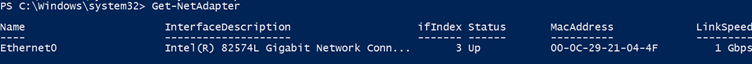
\includegraphics[width=0.85\textwidth,keepaspectratio]{media/9.png}
\caption{Kết quả kiểm tra Network Adapter}
\end{figure}

\begin{lstlisting}[style=powershell]
# Cau hinh IP tinh (neu can test)
New-NetIPAddress -InterfaceAlias "Ethernet" `
  -IPAddress "192.168.244.20" `
  -PrefixLength 24 `
  -DefaultGateway "192.168.244.1"
\end{lstlisting}

\begin{figure}[htbp]
\centering
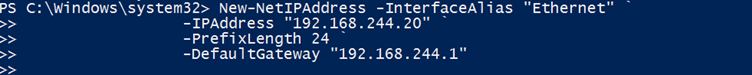
\includegraphics[width=0.85\textwidth,keepaspectratio]{media/10.png}
\caption{Cấu hình IP Address}
\end{figure}

\begin{lstlisting}[style=powershell]
# Cau hinh DNS tro ve Server
Set-DnsClientServerAddress -InterfaceAlias "Ethernet0" `
  -ServerAddresses "192.168.244.10"
\end{lstlisting}

\begin{figure}[htbp]
\centering
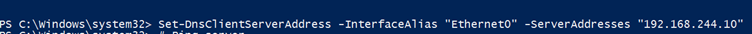
\includegraphics[width=0.85\textwidth,keepaspectratio]{media/11.png}
\caption{Cấu hình DNS Server}
\end{figure}

\textbf{Kết quả kiểm tra:}
\begin{itemize}
    \item[\checkmark] Adapter mạng nhận diện đúng
    \item[\checkmark] IP được cấu hình thành công
    \item[\checkmark] DNS Server được trỏ đúng về 192.168.244.10
\end{itemize}

\subsection{Kiểm tra kết nối}

\begin{lstlisting}[style=powershell]
# Ping toi Server
ping 192.168.244.10
\end{lstlisting}

\begin{figure}[htbp]
\centering
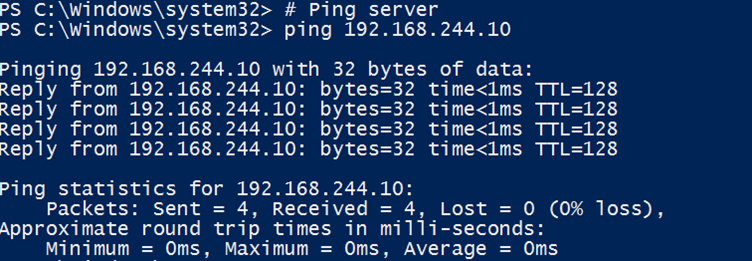
\includegraphics[width=0.85\textwidth,keepaspectratio]{media/12.png}
\caption{Kết quả ping tới Server}
\end{figure}

\begin{lstlisting}[style=powershell]
# Kiem tra phan giai DNS
nslookup ABC.local 192.168.244.10
\end{lstlisting}

\begin{figure}[htbp]
\centering
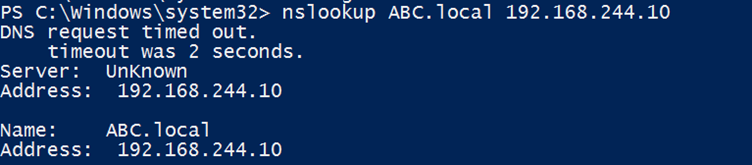
\includegraphics[width=0.85\textwidth,keepaspectratio]{media/13.png}
\caption{Kiểm tra phân giải DNS}
\end{figure}

\textbf{Kết quả:}
\begin{itemize}
    \item[\checkmark] Ping thành công tới Server (0\% loss)
    \item[\checkmark] DNS phân giải đúng domain ABC.local
\end{itemize}

\section{Kiểm tra Join Domain}

\subsection{Thực hiện Join Domain}

\begin{lstlisting}[style=powershell]
# Chay voi quyen Administrator
Add-Computer -DomainName ABC.local -Credential ABC\Administrator -Force
# Password: Manh31102005
Restart-Computer -Force
\end{lstlisting}

\begin{figure}[htbp]
\centering
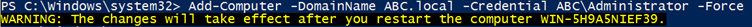
\includegraphics[width=0.85\textwidth,keepaspectratio]{media/14.png}
\caption{Join Domain thành công}
\end{figure}

\textbf{Kết quả:}
\begin{itemize}
    \item[\checkmark] Client join domain thành công
    \item[\checkmark] Máy tự động restart sau khi join
\end{itemize}

\subsection{Đăng nhập với Domain Account}
\textbf{Thông tin đăng nhập:}
\begin{itemize}
    \item \textbf{User Design:} ABC\textbackslash user\_design
    \item \textbf{User Office:} ABC\textbackslash user\_office
    \item \textbf{User Accounting:} ABC\textbackslash user\_accounting
    \item \textbf{Password:} Manh31102005
\end{itemize}

\noindent\textbf{Kết quả:} \checkmark \ Tất cả user đăng nhập thành công

\section{Kiểm tra phân phối máy in tự động (GPO)}

\subsection{Test với user\_office}
\textbf{Đăng nhập:} ABC\textbackslash user\_office

\begin{lstlisting}[style=powershell]
# Cho phep chay script
Set-ExecutionPolicy -Scope Process -ExecutionPolicy Bypass -Force
# Kiem tra Group Membership
whoami /groups | findstr /i grp
\end{lstlisting}

\begin{figure}[htbp]
\centering
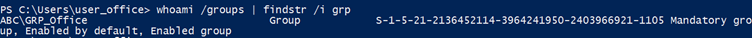
\includegraphics[width=0.85\textwidth,keepaspectratio]{media/15.png}
\caption{Kiểm tra Group Membership của user\_office}
\end{figure}

\textbf{Kết quả kiểm tra Group Membership:}
\begin{itemize}
    \item[\checkmark] User thuộc nhóm GRP\_Office
    \item[\checkmark] Group được phân quyền đúng
\end{itemize}

\begin{lstlisting}[style=powershell]
# Kiem tra may in da duoc map
Get-Printer | Format-Table Name, ShareName
\end{lstlisting}

\begin{figure}[htbp]
\centering
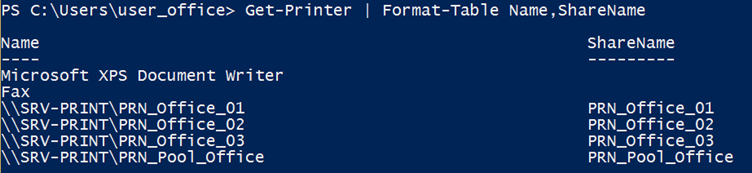
\includegraphics[width=0.85\textwidth,keepaspectratio]{media/16.png}
\caption{Danh sách máy in được map cho user\_office}
\end{figure}

\textbf{Kết quả máy in được map:}
\begin{itemize}
    \item[\checkmark] \textbackslash\textbackslash SRV-PRINT\textbackslash PRN\_Office\_01 - Hiển thị trong danh sách
    \item[\checkmark] \textbackslash\textbackslash SRV-PRINT\textbackslash PRN\_Pool\_Office - Hiển thị trong danh sách
    \item[\checkmark] Không thấy máy in của phòng khác (đúng policy)
\end{itemize}

\subsection{Test với user\_design và user\_accounting}
\textbf{Kết quả user\_design:}
\begin{itemize}
    \item[\checkmark] \textbackslash\textbackslash SRV-PRINT\textbackslash PRN\_Design\_01 được map tự động
    \item[\checkmark] Chỉ thấy máy in của phòng Design
\end{itemize}

\textbf{Kết quả user\_accounting:}
\begin{itemize}
    \item[\checkmark] \textbackslash\textbackslash SRV-PRINT\textbackslash PRN\_Accounting\_01 được map tự động
    \item[\checkmark] Chỉ thấy máy in của phòng Accounting
\end{itemize}

\begin{figure}[htbp]
\centering
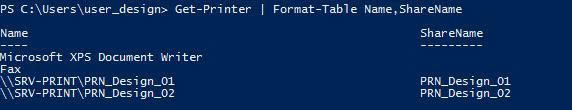
\includegraphics[width=0.7\textwidth,keepaspectratio]{media/89.jpg}
\caption{Máy in được map cho user\_design }
\end{figure}
\begin{figure}[htbp]
\centering
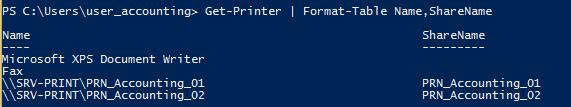
\includegraphics[width=0.7\textwidth,keepaspectratio]{media/90.jpg}
\caption{Máy in được map cho user\_accounting}
\end{figure}
\section{Kiểm tra chức năng in ấn}

\subsection{Test In từ Client (user\_office)}
\textbf{Các bước thực hiện:}
\begin{enumerate}
    \item Mở Notepad trên client
    \item Nhập nội dung: "Test Print - user\_office"
    \item File → Print → Chọn \textbackslash\textbackslash SRV-PRINT\textbackslash PRN\_Office\_01
    \item Nhấn Print
\end{enumerate}

\begin{lstlisting}[style=powershell]
# Kiem tra Print Job tren Client
Get-WmiObject -Class Win32_PrintJob | 
  Select-Object Name, Document, JobId, Owner, TotalPages, Status | 
  Format-Table -AutoSize
\end{lstlisting}

\begin{figure}[htbp]
\centering
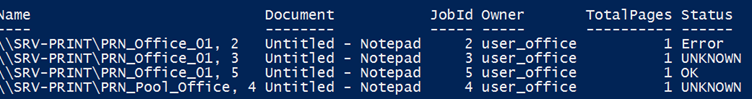
\includegraphics[width=0.85\textwidth,keepaspectratio]{media/29.png}
\caption{Print Job trên Client}
\end{figure}

\textbf{Kết quả:}
\begin{itemize}
    \item[\checkmark] Print job được tạo thành công
    \item[\checkmark] Owner: ABC\textbackslash user\_office
    \item[\checkmark] Document name: "Untitled - Notepad"
    \item[\checkmark] Status: Đang xử lý hoặc hoàn thành
\end{itemize}

\subsection{Kiểm tra Queue trên Server}

\begin{lstlisting}[style=powershell]
# Kiem tra queue cua may in PRN_Office_01
Get-PrintJob -PrinterName "PRN_Office_01" | 
  Select PrinterName, JobId, JobStatus, Owner, DocumentName, SubmittedTime | 
  Format-Table -AutoSize
\end{lstlisting}

\begin{figure}[htbp]
\centering
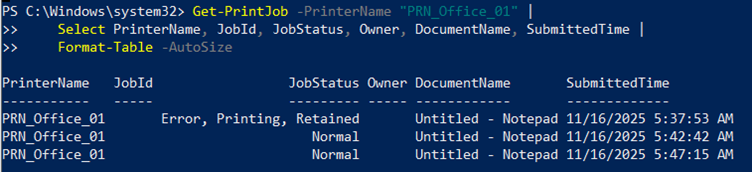
\includegraphics[width=0.85\textwidth,keepaspectratio]{media/28.png}
\caption{Queue của máy in PRN\_Office\_01 trên Server}
\end{figure}

\textbf{Kết quả:}
\begin{itemize}
    \item[\checkmark] Job xuất hiện trong queue của Server
    \item[\checkmark] PrinterName: PRN\_Office\_01
    \item[\checkmark] Owner: ABC\textbackslash user\_office
    \item[\checkmark] SubmittedTime: [Thời gian chính xác]
    \item[\checkmark] JobStatus: Normal/Printing
\end{itemize}

\section{Kiểm tra Logging \& Audit}

\subsection{Event Log}

\begin{lstlisting}[style=powershell]
# Kiem tra Print Service Event Log
Get-EventLog -LogName "Print Service Log" -Newest 20
\end{lstlisting}

\begin{figure}[htbp]
\centering
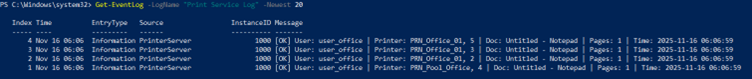
\includegraphics[width=0.85\textwidth,keepaspectratio]{media/27.png}
\caption{Event Log của Print Service}
\end{figure}

\textbf{Kết quả:}
\begin{itemize}
    \item[\checkmark] Event ID 307 được ghi nhận (Document printed)
    \item[\checkmark] Thông tin đầy đủ: User, Printer, Document, Time
    \item[\checkmark] Event Log hoạt động bình thường
\end{itemize}

\section{Kiểm tra thứ tự xử lý Queue}

\subsection{Test với 3 User đồng thời}
\textbf{Thứ tự thực hiện:}
\begin{enumerate}
    \item \textbf{Client 1 (user\_accounting):} In "Test Accounting" → PRN\_Accounting\_01
    \item \textbf{Client 2 (user\_design):} In "Test Design" → PRN\_Design\_01
    \item \textbf{Client 3 (user\_office):} In "Test Office" → PRN\_Pool\_Office
\end{enumerate}

\begin{lstlisting}[style=powershell]
# Kiem tra tren Server
Get-WmiObject Win32_PrintJob | 
  Select-Object Name, JobId, Owner, Status, TimeSubmitted | 
  Format-Table -AutoSize
\end{lstlisting}

\begin{figure}[htbp]
\centering
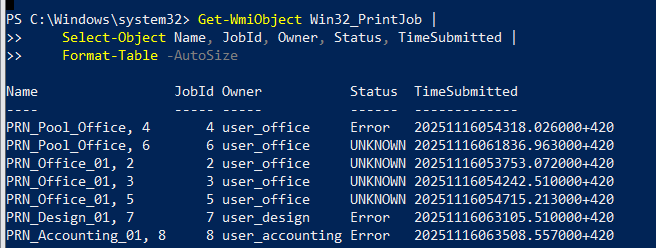
\includegraphics[width=0.75\textwidth,keepaspectratio]{media/26.png}
\caption{Thứ tự Job trong Queue của Server}
\end{figure}

\textbf{Kết quả quan sát:}
\begin{itemize}
    \item[\checkmark] Job từ Accounting xuất hiện đầu tiên
    \item[\checkmark] Job từ Design xuất hiện thứ hai
    \item[\checkmark] Job từ Office xuất hiện cuối cùng
    \item[\checkmark] Thứ tự xử lý: Accounting → Design → Office (đúng priority)
\end{itemize}

\noindent\textbf{Nhận xét:} Hệ thống xử lý đúng thứ tự ưu tiên đã cấu hình.

\section{Kiểm tra chức năng báo cáo}

\subsection{Báo cáo theo User}

\subsubsection{Báo cáo user\_design}
\begin{lstlisting}[style=powershell]
Export-UserPrinterHistory -Username user_design
\end{lstlisting}

\begin{figure}[htbp]
\centering
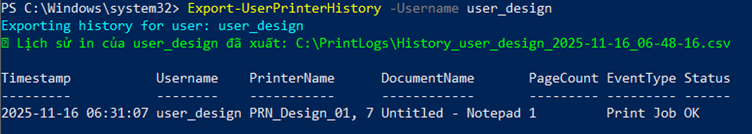
\includegraphics[width=0.85\textwidth,keepaspectratio]{media/25.png}
\caption{Báo cáo lịch sử in của user\_design}
\end{figure}

\textbf{Kết quả:}
\begin{itemize}
    \item[\checkmark] File CSV được tạo tại C:\textbackslash PrintReports\textbackslash
    \item[\checkmark] Nội dung chứa: User, Printer, Document, Pages, Time
    \item[\checkmark] Dữ liệu chính xác với các job đã in
\end{itemize}

\subsubsection{Báo cáo user\_accounting}
\begin{lstlisting}[style=powershell]
Export-UserPrinterHistory -Username user_accounting
\end{lstlisting}

\begin{figure}[htbp]
\centering
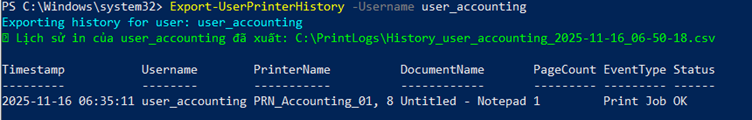
\includegraphics[width=0.85\textwidth,keepaspectratio]{media/24.png}
\caption{Báo cáo lịch sử in của user\_accounting}
\end{figure}

\textbf{Kết quả:}
\begin{itemize}
    \item[\checkmark] File CSV được xuất thành công
    \item[\checkmark] Hiển thị đầy đủ lịch sử in của user\_accounting
    \item[\checkmark] Dữ liệu audit đầy đủ
\end{itemize}

\subsubsection{Báo cáo user\_office}
\begin{lstlisting}[style=powershell]
Export-UserPrinterHistory -Username user_office
\end{lstlisting}

\begin{figure}[htbp]
\centering
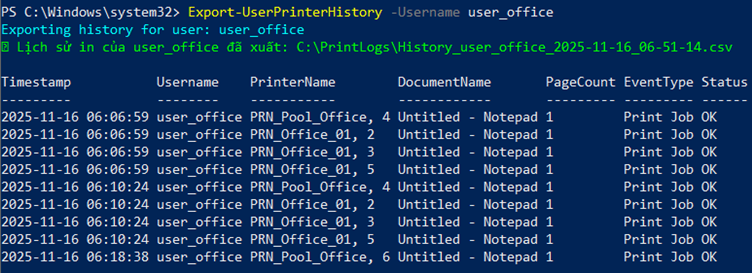
\includegraphics[width=0.85\textwidth,keepaspectratio]{media/23.png}
\caption{Báo cáo lịch sử in của user\_office}
\end{figure}

\textbf{Kết quả:}
\begin{itemize}
    \item[\checkmark] Báo cáo xuất thành công
    \item[\checkmark] Bao gồm tất cả các job từ PRN\_Office\_01 và PRN\_Pool\_Office
    \item[\checkmark] Thông tin chi tiết và chính xác
\end{itemize}

\subsection{Báo cáo 30 ngày}

\begin{lstlisting}[style=powershell]
# Xuat bao cao tong hop 30 ngay
Export-MonthlyPrintReport
\end{lstlisting}

\begin{figure}[htbp]
\centering
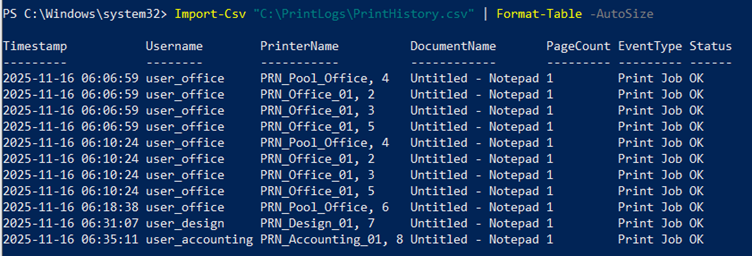
\includegraphics[width=0.85\textwidth,keepaspectratio]{media/22.png}
\caption{Báo cáo tổng hợp 30 ngày}
\end{figure}

\textbf{Kết quả:}
\begin{itemize}
    \item[\checkmark] File CSV tổng hợp được tạo
    \item[\checkmark] Bao gồm tất cả user và tất cả máy in
    \item[\checkmark] Thống kê đầy đủ: tổng số trang, số job, phân bố theo phòng ban
    \item[\checkmark] Định dạng phù hợp cho phân tích và audit
\end{itemize}

\section{Kiểm tra chức năng Troubleshooting}

\subsection{Kiểm tra tổng quan hệ thống}

\begin{lstlisting}[style=powershell]
Get-PrinterServerStatus
\end{lstlisting}

\begin{figure}[htbp]
\centering
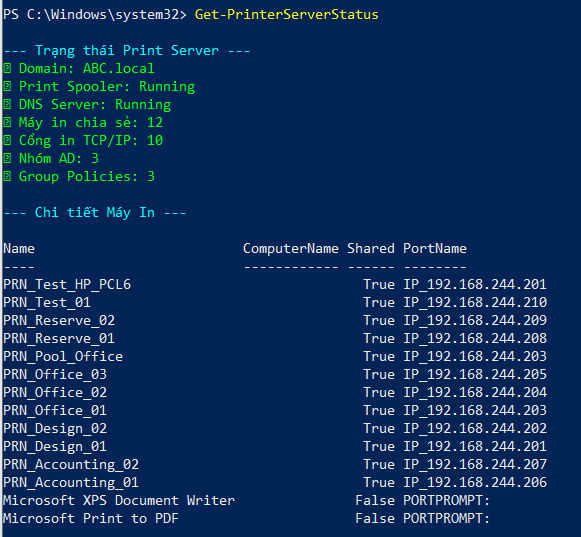
\includegraphics[width=0.75\textwidth,keepaspectratio]{media/21.png}
\caption{Trạng thái tổng quan của Print Server}
\end{figure}

\textbf{Kết quả:}
\begin{itemize}
    \item[\checkmark] Hiển thị tất cả máy in trong hệ thống
    \item[\checkmark] Trạng thái mỗi máy: Online/Offline
    \item[\checkmark] Số job đang chờ trong queue
    \item[\checkmark] Thông tin driver và port
    \item[\checkmark] Tổng quan toàn diện về Print Server
\end{itemize}

\subsection{Test kết nối tất cả máy in}

\begin{lstlisting}[style=powershell]
Test-AllPrinterConnections
\end{lstlisting}

\begin{figure}[htbp]
\centering
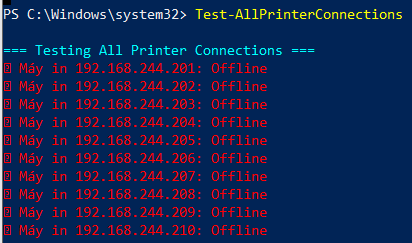
\includegraphics[width=0.6\textwidth,keepaspectratio]{media/20.png}
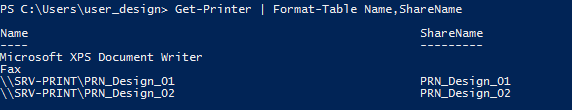
\includegraphics[width=0.6\textwidth,keepaspectratio]{media/77.png}
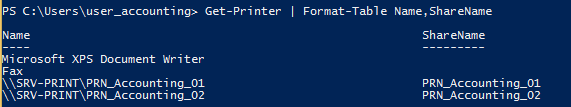
\includegraphics[width=0.6\textwidth,keepaspectratio]{media/78.png}
\caption{Kiểm tra kết nối tất cả máy in}
\end{figure}

\textbf{Kết quả:}
\begin{itemize}
    \item[\checkmark] PRN\_Design\_01: Online \checkmark
    \item[\checkmark] PRN\_Office\_01: Online \checkmark
    \item[\checkmark] PRN\_Pool\_Office: Online \checkmark
    \item[\checkmark] PRN\_Accounting\_01: Online \checkmark
    \item[\checkmark] Tất cả máy in phản hồi bình thường
\end{itemize}


\subsection{Thông tin chi tiết máy in}

\begin{lstlisting}[style=powershell]
Get-PrinterDetailedInfo -PrinterName "PRN_Design_01"
Get-PrinterDetailedInfo -PrinterName "PRN_Office_01"
Get-PrinterDetailedInfo -PrinterName "PRN_Accounting_01"
\end{lstlisting}

\textbf{Kết quả:}
\begin{itemize}
    \item[\checkmark] Hiển thị đầy đủ: Name, Status, Driver, Port, ShareName
    \item[\checkmark] Job count hiện tại
    \item[\checkmark] Thông tin cấu hình chi tiết
    \item[\checkmark] Trạng thái sẵn sàng in
\end{itemize}

\section{Tổng kết kết quả kiểm tra}

\subsection{Các chức năng đạt yêu cầu}

\begin{table}[htbp]
\centering\small
\begin{tabular}{|c|p{5.5cm}|c|p{3.5cm}|}
\hline
\textbf{STT} & \textbf{Chức năng} & \textbf{Kết quả} & \textbf{Ghi chú} \\ \hline
1 & Cấu hình mạng và DNS & \checkmark \ PASS & Kết nối ổn định \\ \hline
2 & Join Domain & \checkmark \ PASS & Tất cả client join OK \\ \hline
3 & Phân phối máy in qua GPO & \checkmark \ PASS & Đúng policy \\ \hline
4 & Chức năng in ấn & \checkmark \ PASS & In thành công \\ \hline
5 & Print Queue Management & \checkmark \ PASS & Thứ tự ưu tiên đúng \\ \hline
6 & Event Logging & \checkmark \ PASS & Event ID 307 đầy đủ \\ \hline
7 & Báo cáo theo User & \checkmark \ PASS & CSV xuất chính xác \\ \hline
8 & Báo cáo 30 ngày & \checkmark \ PASS & Tổng hợp đầy đủ \\ \hline
9 & Monitoring \& Status & \checkmark \ PASS & Hiển thị real-time \\ \hline
10 & Troubleshooting Tools & \checkmark \ PASS & Tất cả hoạt động \\ \hline
\end{tabular}
\caption{Bảng tổng kết kết quả kiểm tra}
\end{table}

\subsection{Đánh giá tổng quan}

\textbf{Điểm mạnh:}
\begin{itemize}
    \item Hệ thống hoạt động ổn định và đúng thiết kế
    \item Phân quyền máy in chính xác theo OU/Group
    \item Logging và audit đầy đủ, đáp ứng yêu cầu giám sát
    \item Báo cáo xuất file CSV tiện lợi cho phân tích
    \item Các function quản lý và troubleshooting hiệu quả
    \item Thứ tự xử lý job theo priority hoạt động đúng
\end{itemize}
\vspace{\baselineskip}

\chapter{\textbf{Kết luận và Nhận xét}}

\section{Kết Quả Đạt Được}

\begin{itemize}
    \item[\checkmark] \textbf{Triển khai Print Server hoàn toàn không sử dụng GUI} -- tất cả qua PowerShell CLI
    \item[\checkmark] \textbf{Phân quyền theo nhóm phòng ban} -- chỉ user đúng group mới truy cập máy in
    \item[\checkmark] \textbf{Máy in Pool tự động chia tải} -- 7 máy in vật lý được quản lý bởi 1 máy in ảo
    \item[\checkmark] \textbf{Độ ưu tiên được thiết lập rõ ràng} -- máy in kế toán ưu tiên cao nhất (75)
    \item[\checkmark] \textbf{Logging \& báo cáo chi tiết} -- truy vết lịch sử in ấn theo từng user
    \item[\checkmark] \textbf{Tự động phân phối máy in} -- client nhận máy in khi join domain qua GPO
\end{itemize}

\section{Công Nghệ \& Công Cụ Sử Dụng}

\begin{itemize}
    \item \textbf{Windows Server 2019 Datacenter}
    \item \textbf{Active Directory Domain Services (AD DS)}
    \item \textbf{Print Server Role}
    \item \textbf{PowerShell 5.0+} (CLI -- không dùng GUI)
    \item \textbf{Group Policy (GPO)} -- triển khai qua lệnh
    \item \textbf{ICACLS} -- phân quyền NTFS
    \item \textbf{Event Viewer Logs} -- giám sát
\end{itemize}

\section{Giá Trị Doanh Nghiệp}

\begin{itemize}
    \item \textbf{Tiết kiệm chi phí:} Quản lý tập trung, giảm lỗi cấu hình thủ công
    \item \textbf{Bảo mật cao:} Phân quyền rõ ràng, truy vết hoạt động chi tiết
    \item \textbf{Hiệu suất tốt:} Pool và priority đảm bảo máy in quan trọng luôn ưu tiên
    \item \textbf{Dễ bảo trì:} Tự động hóa qua script, dễ scaling khi phát triển công ty
\end{itemize}

\chapter{\textbf{Phụ lục, Tham khảo}}

\section{Danh sách lệnh PowerShell}

\begin{table}[htbp]
\centering\small
\begin{tabular}{|l|p{8cm}|}
\hline
\textbf{Lệnh} & \textbf{Chức năng} \\ \hline
Add-PrinterPort & Tạo port máy in \\ \hline
Add-Printer & Tạo máy in \\ \hline
Set-Printer & Sửa đặc tính máy in \\ \hline
Get-Printer & Liệt kê máy in \\ \hline
Get-PrintJob & Xem hàng đợi in \\ \hline
Remove-PrintJob & Xóa job \\ \hline
Restart-Service Spooler & Khởi động lại dịch vụ in \\ \hline
New-ADUser & Tạo user \\ \hline
New-ADGroup & Tạo group \\ \hline
Add-ADGroupMember & Thêm user vào group \\ \hline
Get-WinEvent & Truy vấn Event Log \\ \hline
icacls & Phân quyền NTFS \\ \hline
gpupdate /force & Cập nhật GPO \\ \hline
\end{tabular}
\caption{Danh sách lệnh PowerShell chính}
\end{table}

\section{Port và Protocol}

\begin{table}[htbp]
\centering\small
\begin{tabular}{|l|l|p{5.5cm}|}
\hline
\textbf{Port} & \textbf{Protocol} & \textbf{Dịch vụ} \\ \hline
9100 & TCP & JetDirect (Printer) \\ \hline
445 & TCP & SMB Sharing \\ \hline
139 & TCP/UDP & NetBIOS \\ \hline
53 & TCP/UDP & DNS \\ \hline
88 & TCP & Kerberos \\ \hline
389 & TCP/UDP & LDAP \\ \hline
\end{tabular}
\caption{Port và giao thức sử dụng}
\end{table}

\section{Tài liệu tham khảo}

\begin{itemize}
    \item Microsoft Learn: Print Server Role
    \item Active Directory Best Practices
    \item PowerShell PrintManagement Module Documentation
    \item Group Policy Management Console Guide
\end{itemize}


\clearpage

% --- BACKMATTER ---
% \input{backmatter/05_tai_lieu_tham_khao.tex}

\end{document}
